\documentclass[../main.tex]{subfiles}

\begin{document}

\newpage
\section{Descriptive statistics}

\subsection{Data on the S\&P 500 index}

From the data obtained, we will derive three different quantities to examine.

\subsubsection{Maximum change}

We will call the first quantity maximum change or hml (\textit{high-minus-low}), and calculate it using the formula:

\[ \text{hml} = (\,\text{highest price during the day}\,) - (\,\text{lowest price during the day}
\,) \]

Its representation as a time series is:

\begin{figure}[H]
    \centering
    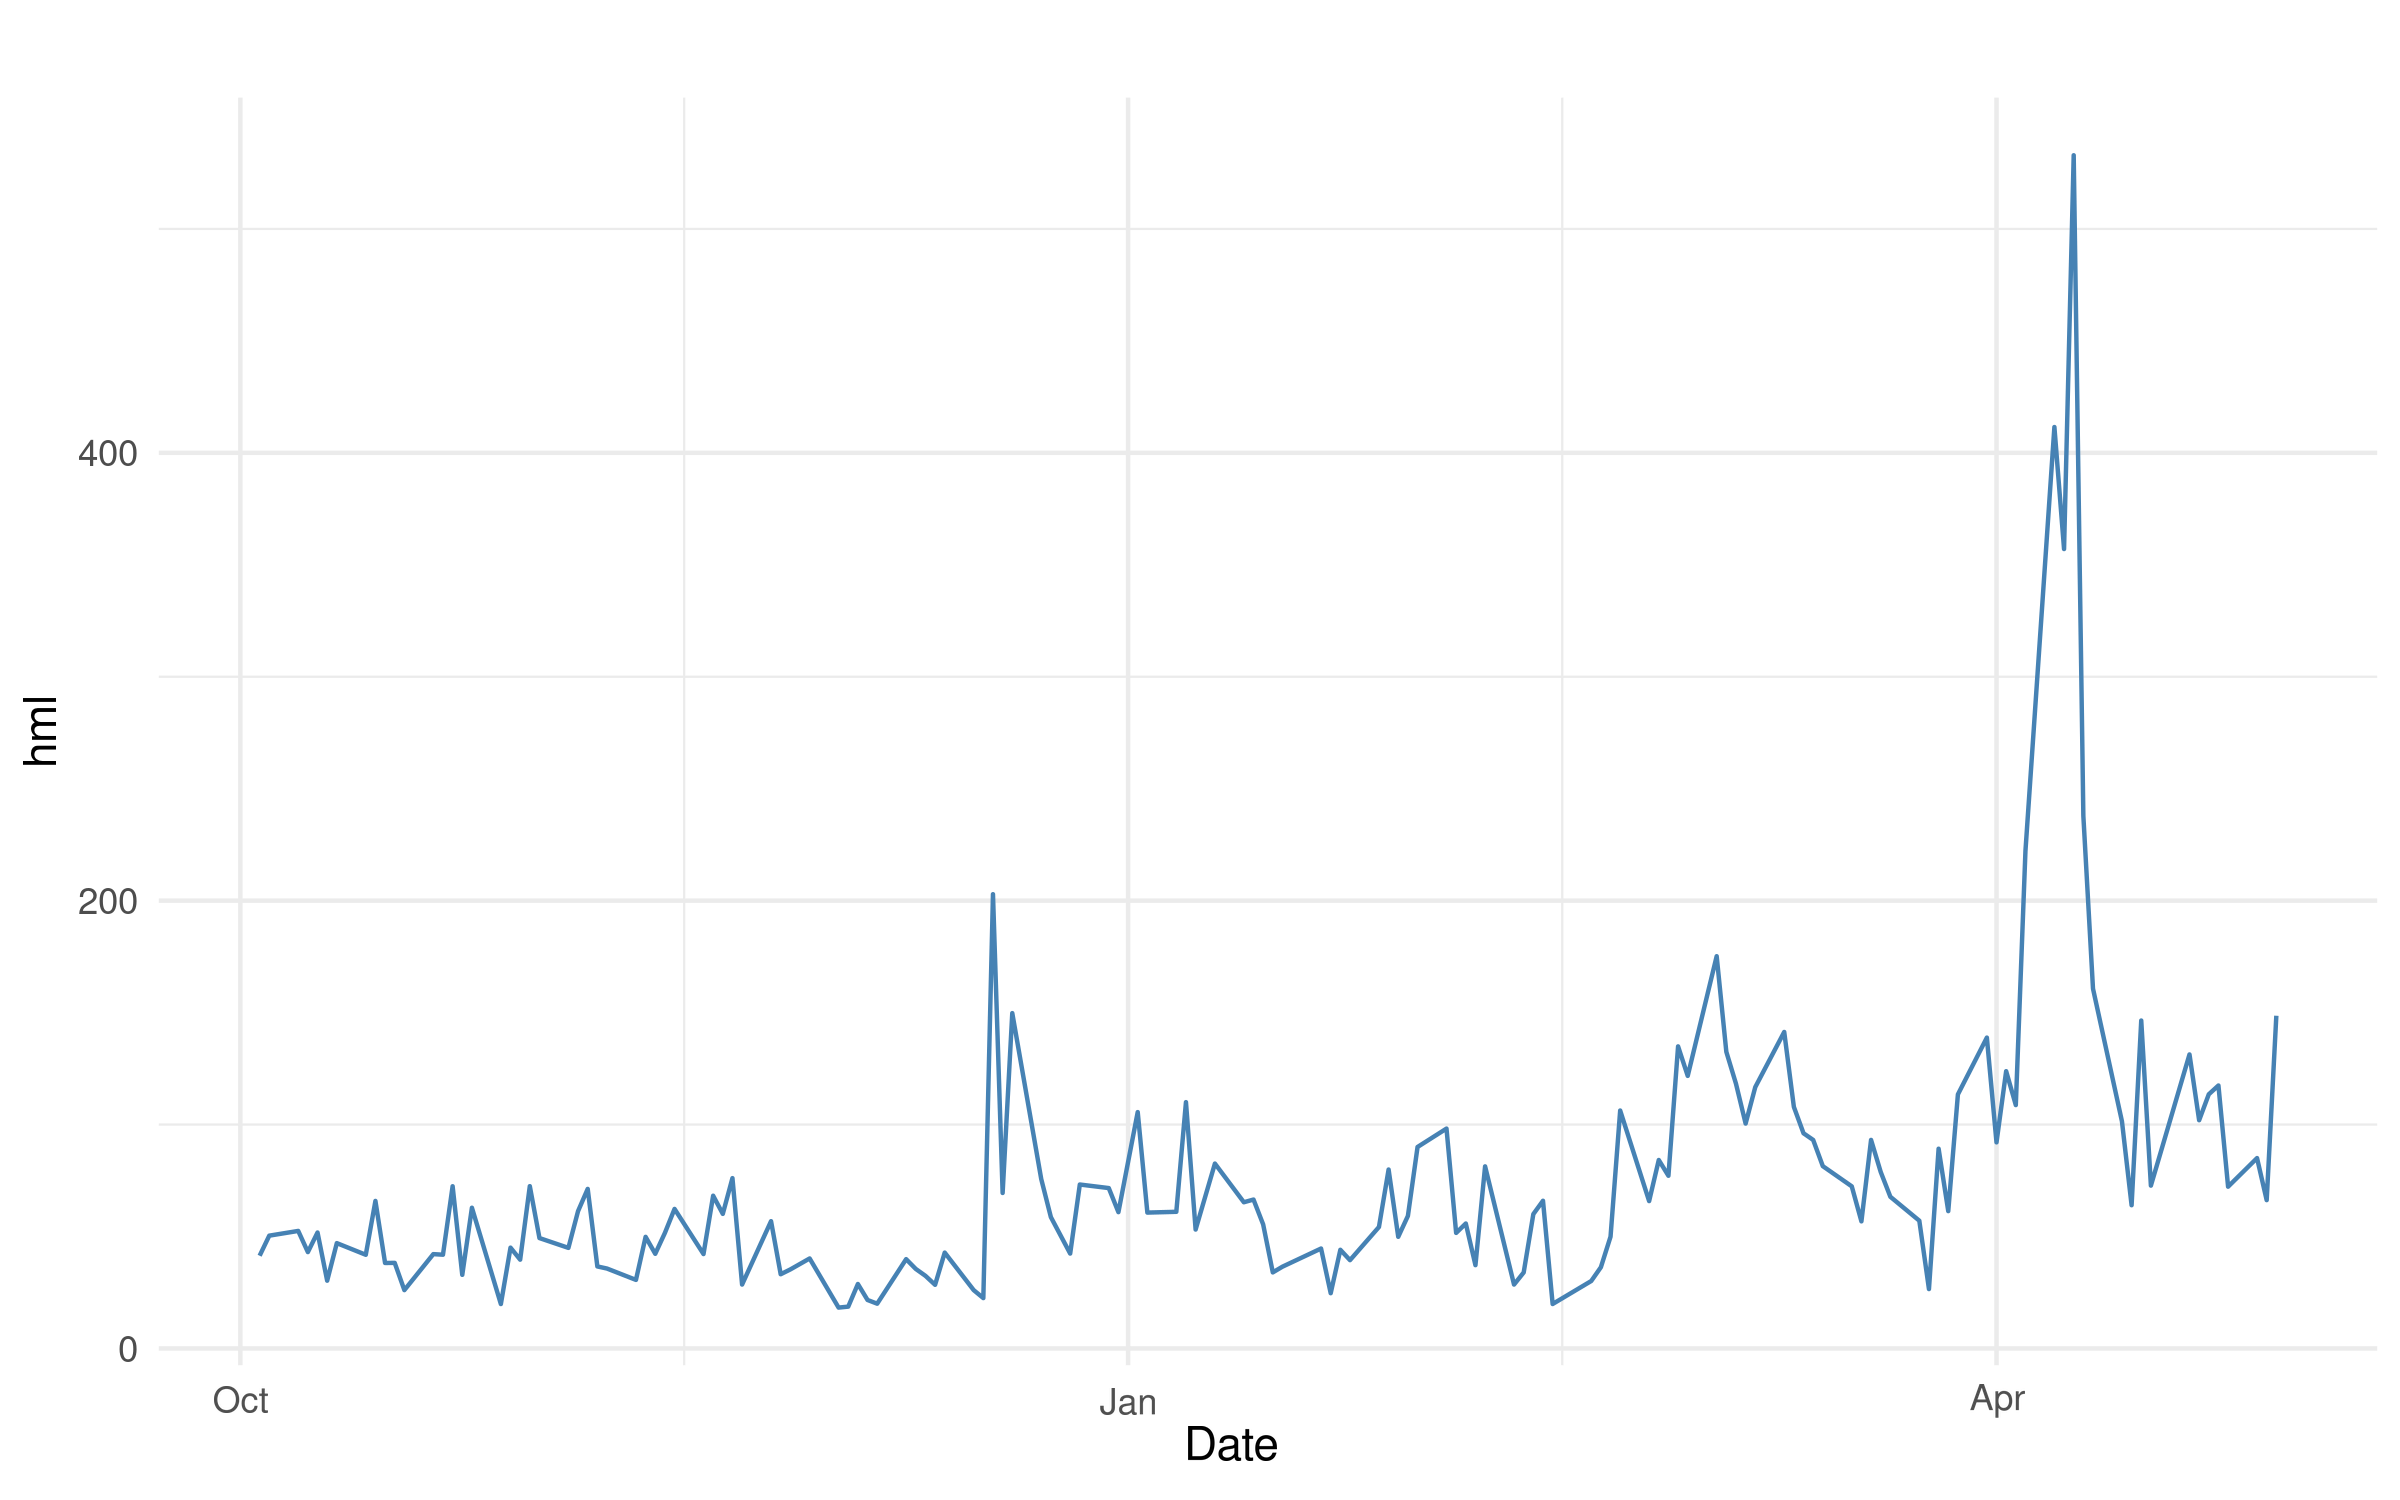
\includegraphics[width=0.8\textwidth]{../pavic_r/hml_timeseries.png}
    \caption{hml during the period examined}
    \label{fig:volatilnost_timeseries}
\end{figure}

The five-number summary is:

\begin{align*}
(x_0(v), q_L(v), m(v), q_U(v), x_{(n)}(v)) &= (18.25,\; 40.80,\; 60.88,\; 91.01,\; 532.91)
\end{align*}

\begin{figure}[H]
    \centering
    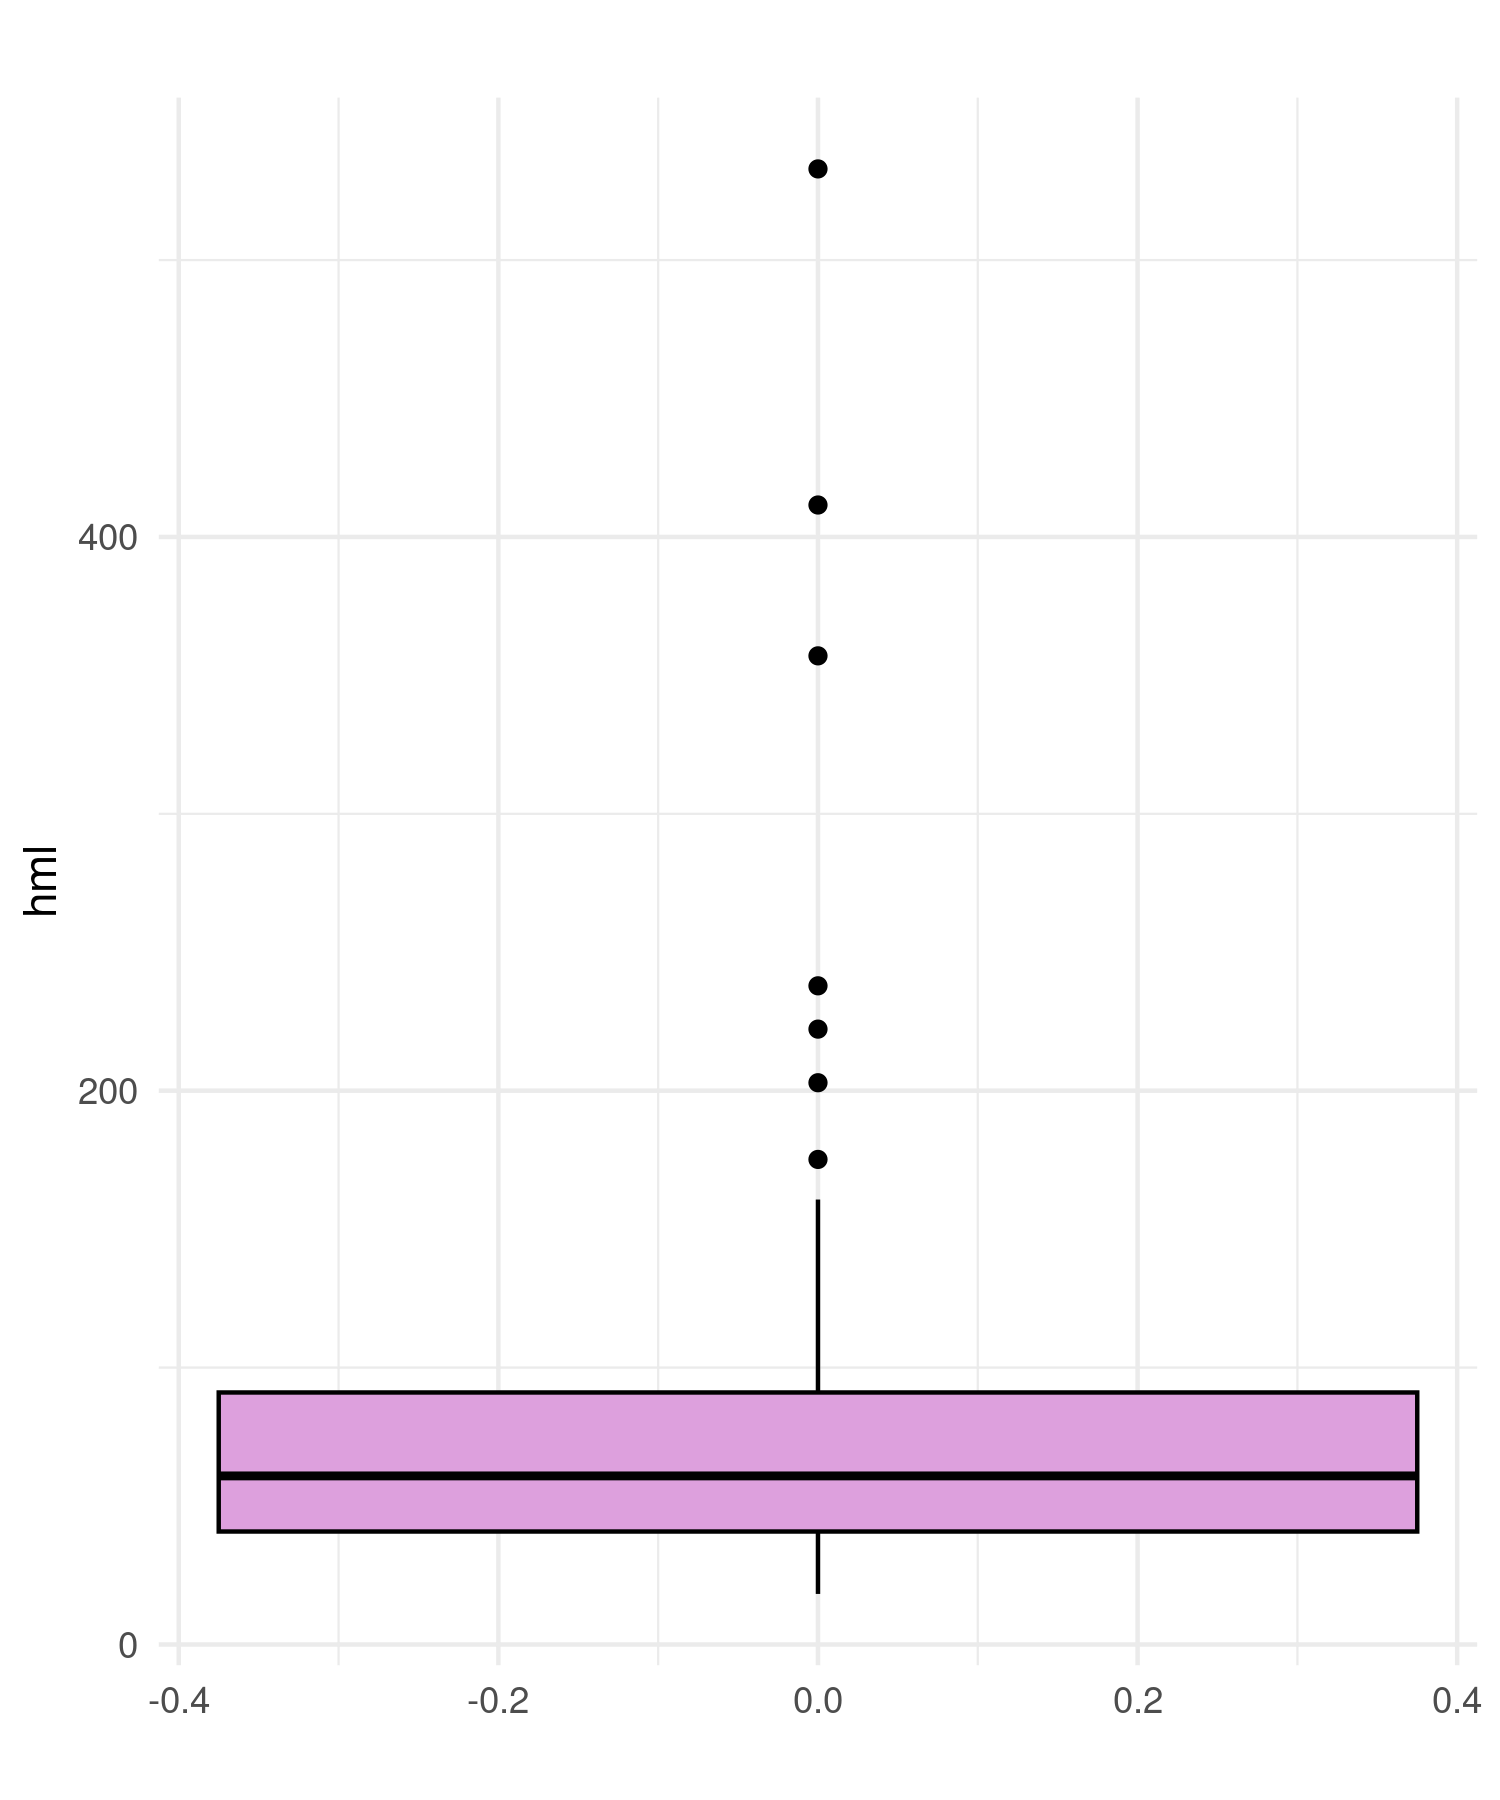
\includegraphics[width=0.4\textwidth]{../pavic_r/hml_boxplot.png}
    \caption{Boxplot}
    \label{fig:hml_boxplot}
\end{figure}

The boxplot shows many outliers, which is to be expected. During the period examined, several events had a huge effect on the market, including:
\begin{itemize}
\item Trump's election as president
\item Trump's inauguration
\item Trump's introduction of tariffs
\end{itemize}

A natural question is which distribution the hml of a trading day comes from. To investigate this further, we plotted its histogram and the histogram of its logarithm. This produced the following plots:

\begin{figure}[H]
  \centering
  \begin{subfigure}[b]{0.48\textwidth}
    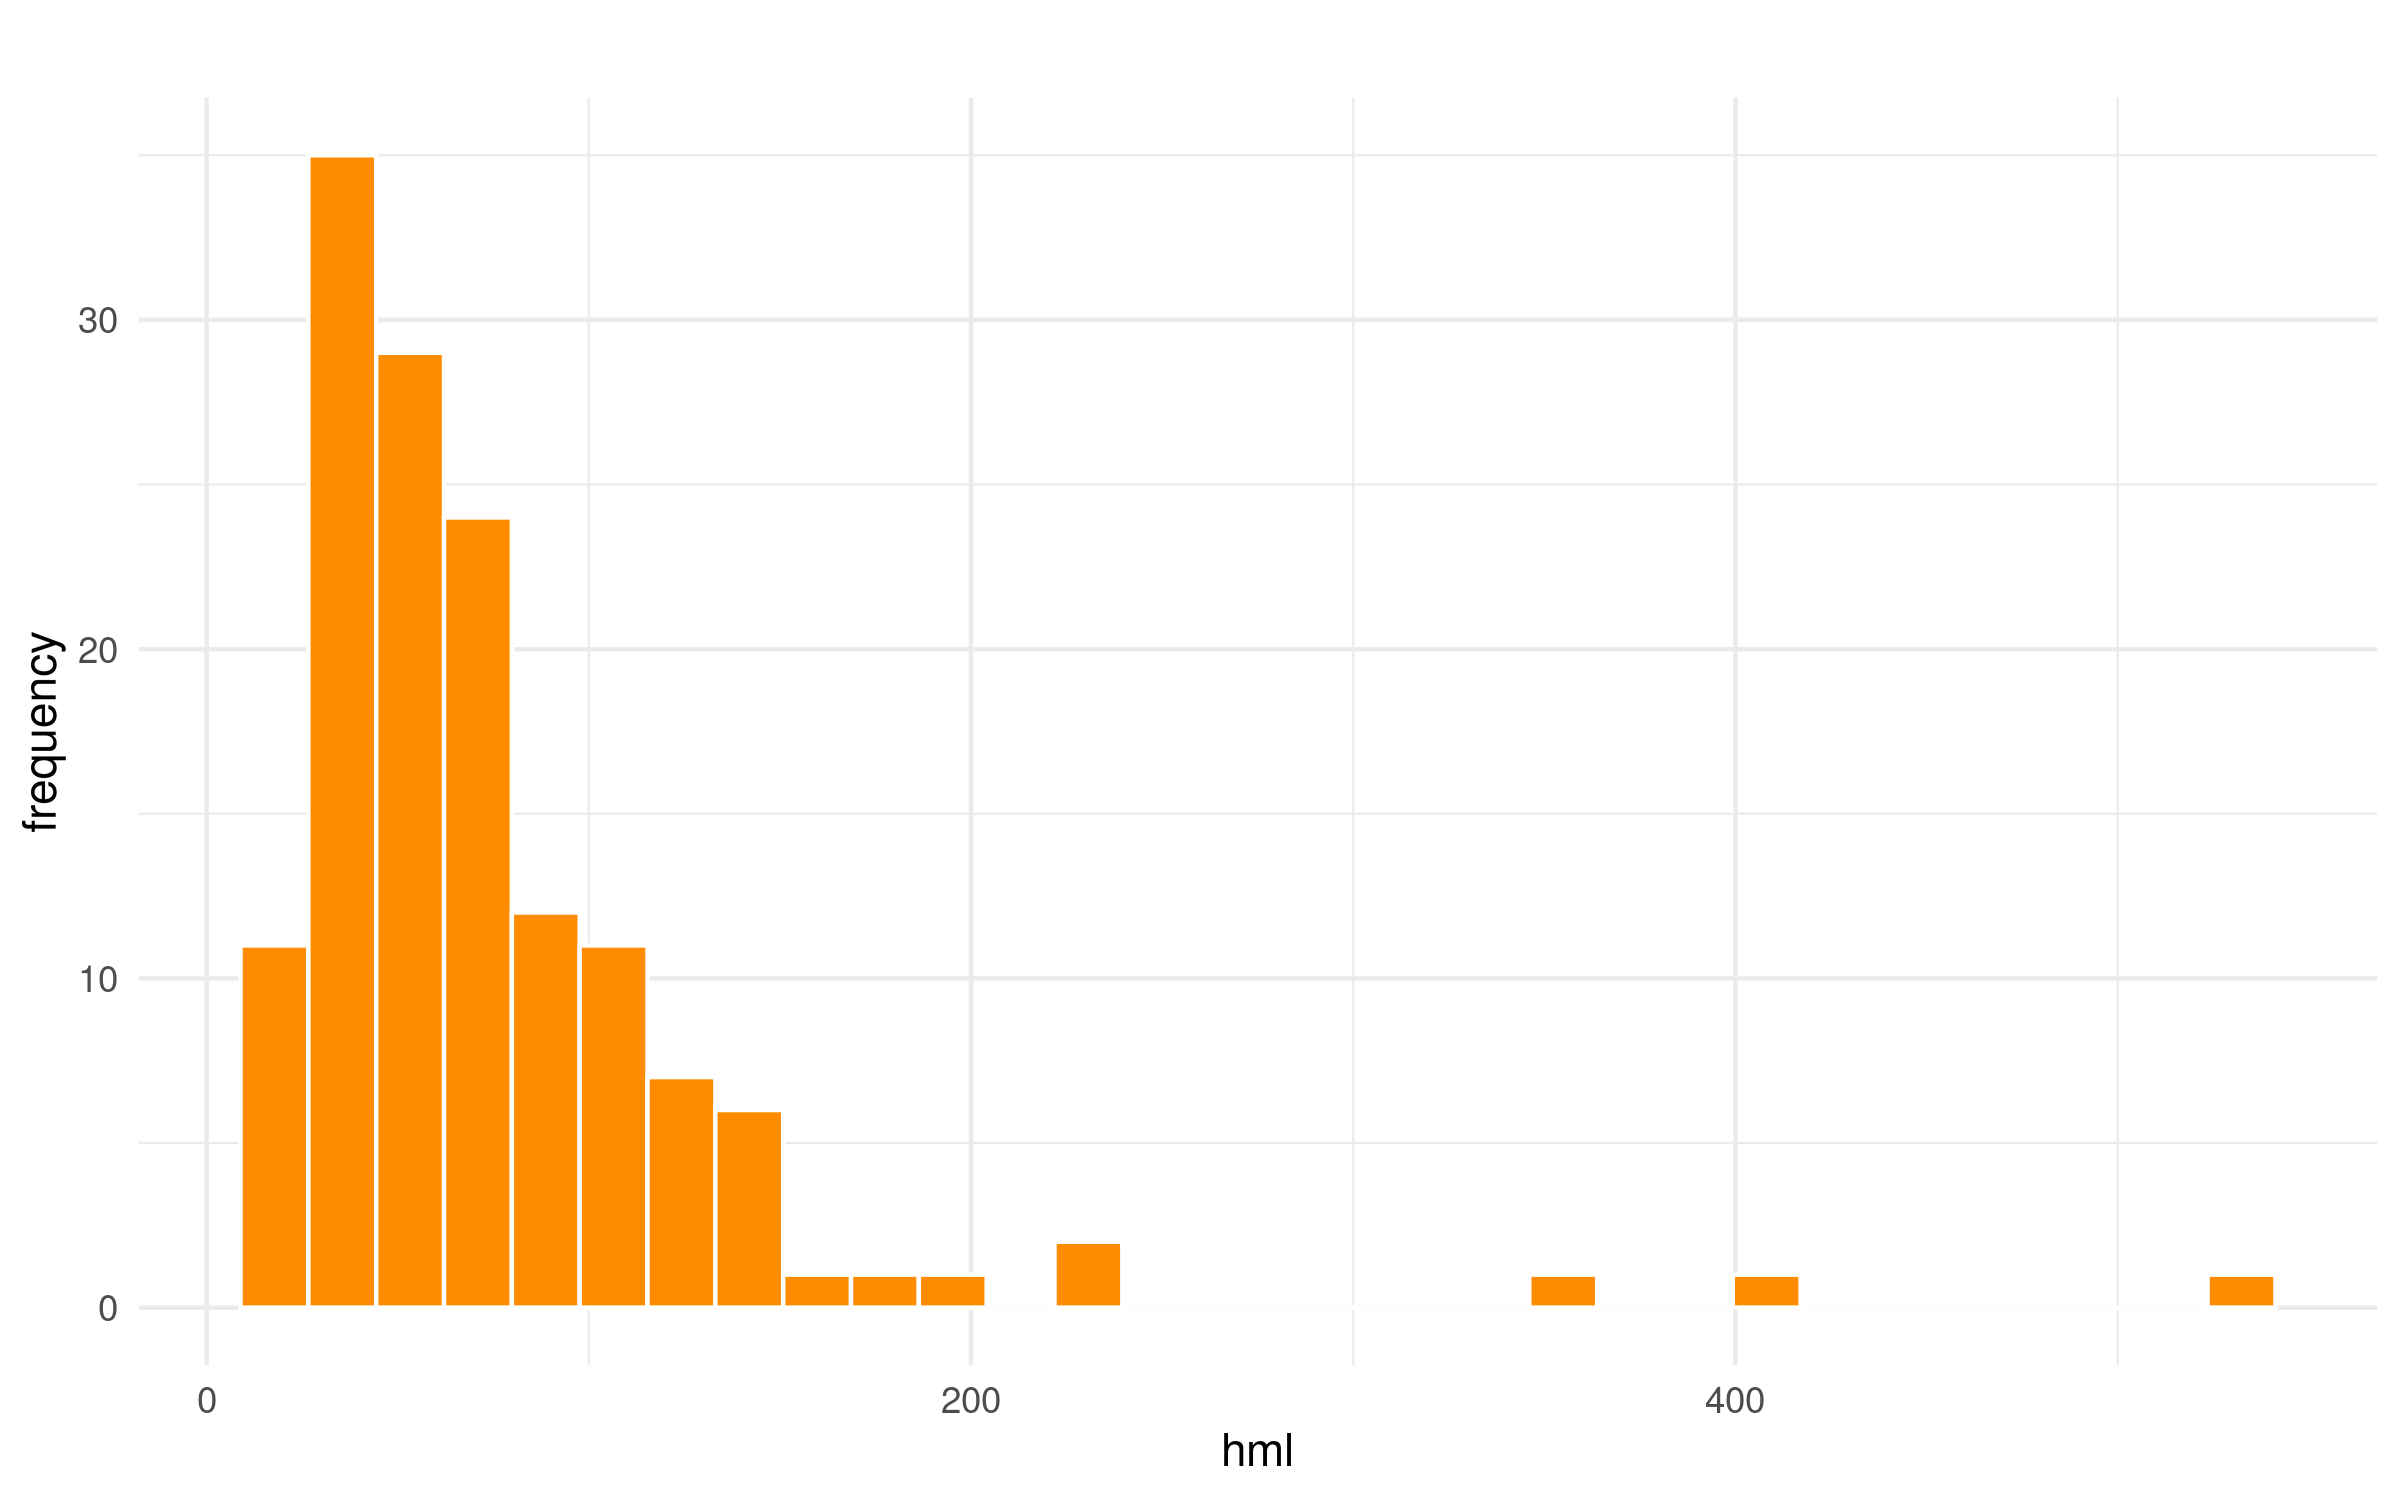
\includegraphics[width=\linewidth]{../pavic_r/hml_histogram.png}
    \caption{Histogram of hml during the period examined}
    \label{fig:hml_histogram}
  \end{subfigure}
  \hfill
  \begin{subfigure}[b]{0.48\textwidth}
    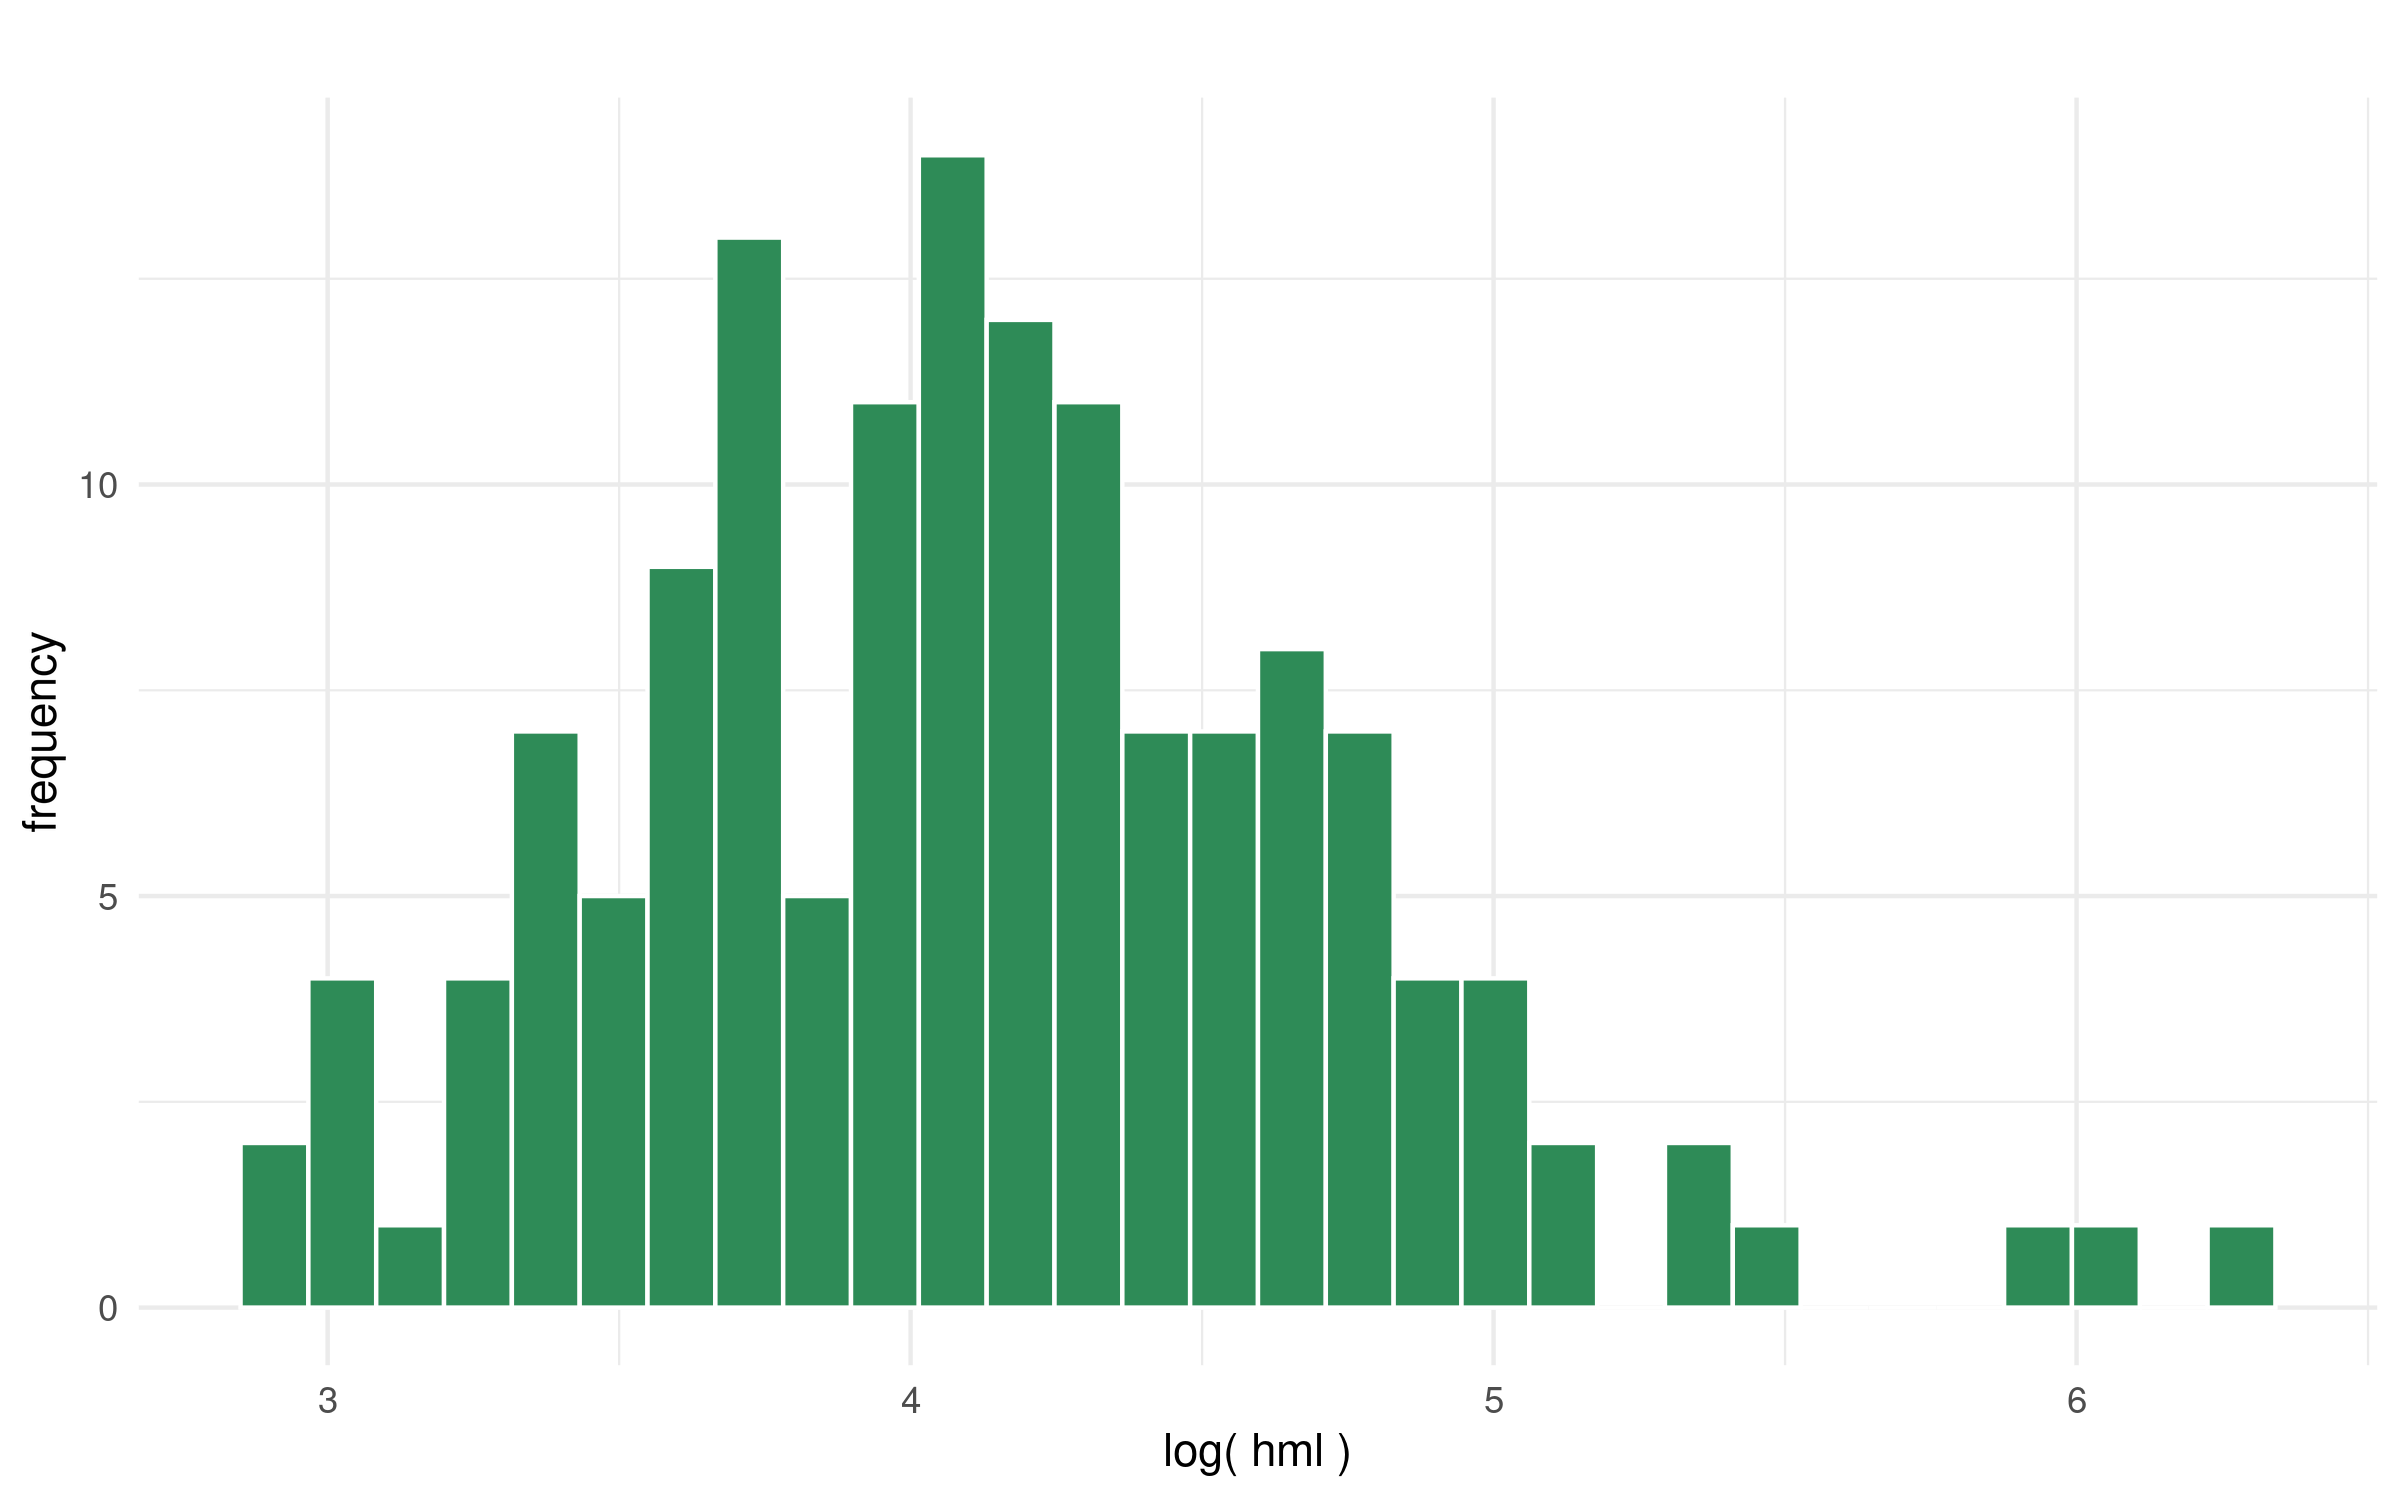
\includegraphics[width=\linewidth]{../pavic_r/hml_loghistogram.png}
    \caption{Histogram of log(hml) during the period examined}
    \label{fig:hml_loghistogram}
  \end{subfigure}
  \caption{Histograms of hml}
  \label{fig:histograms}
\end{figure}

After examining panel (b), we decided to test whether hml follows a log-normal distribution. Specifically, we performed a test for the MLE given by the parameters

\[ \hat{\mu} = 4.1276 \;\; \hat{\sigma}^2 = 0.3814 \]

The distribution is shown below, overlaid with the theoretical curve:

\begin{figure}[H]
    \centering
    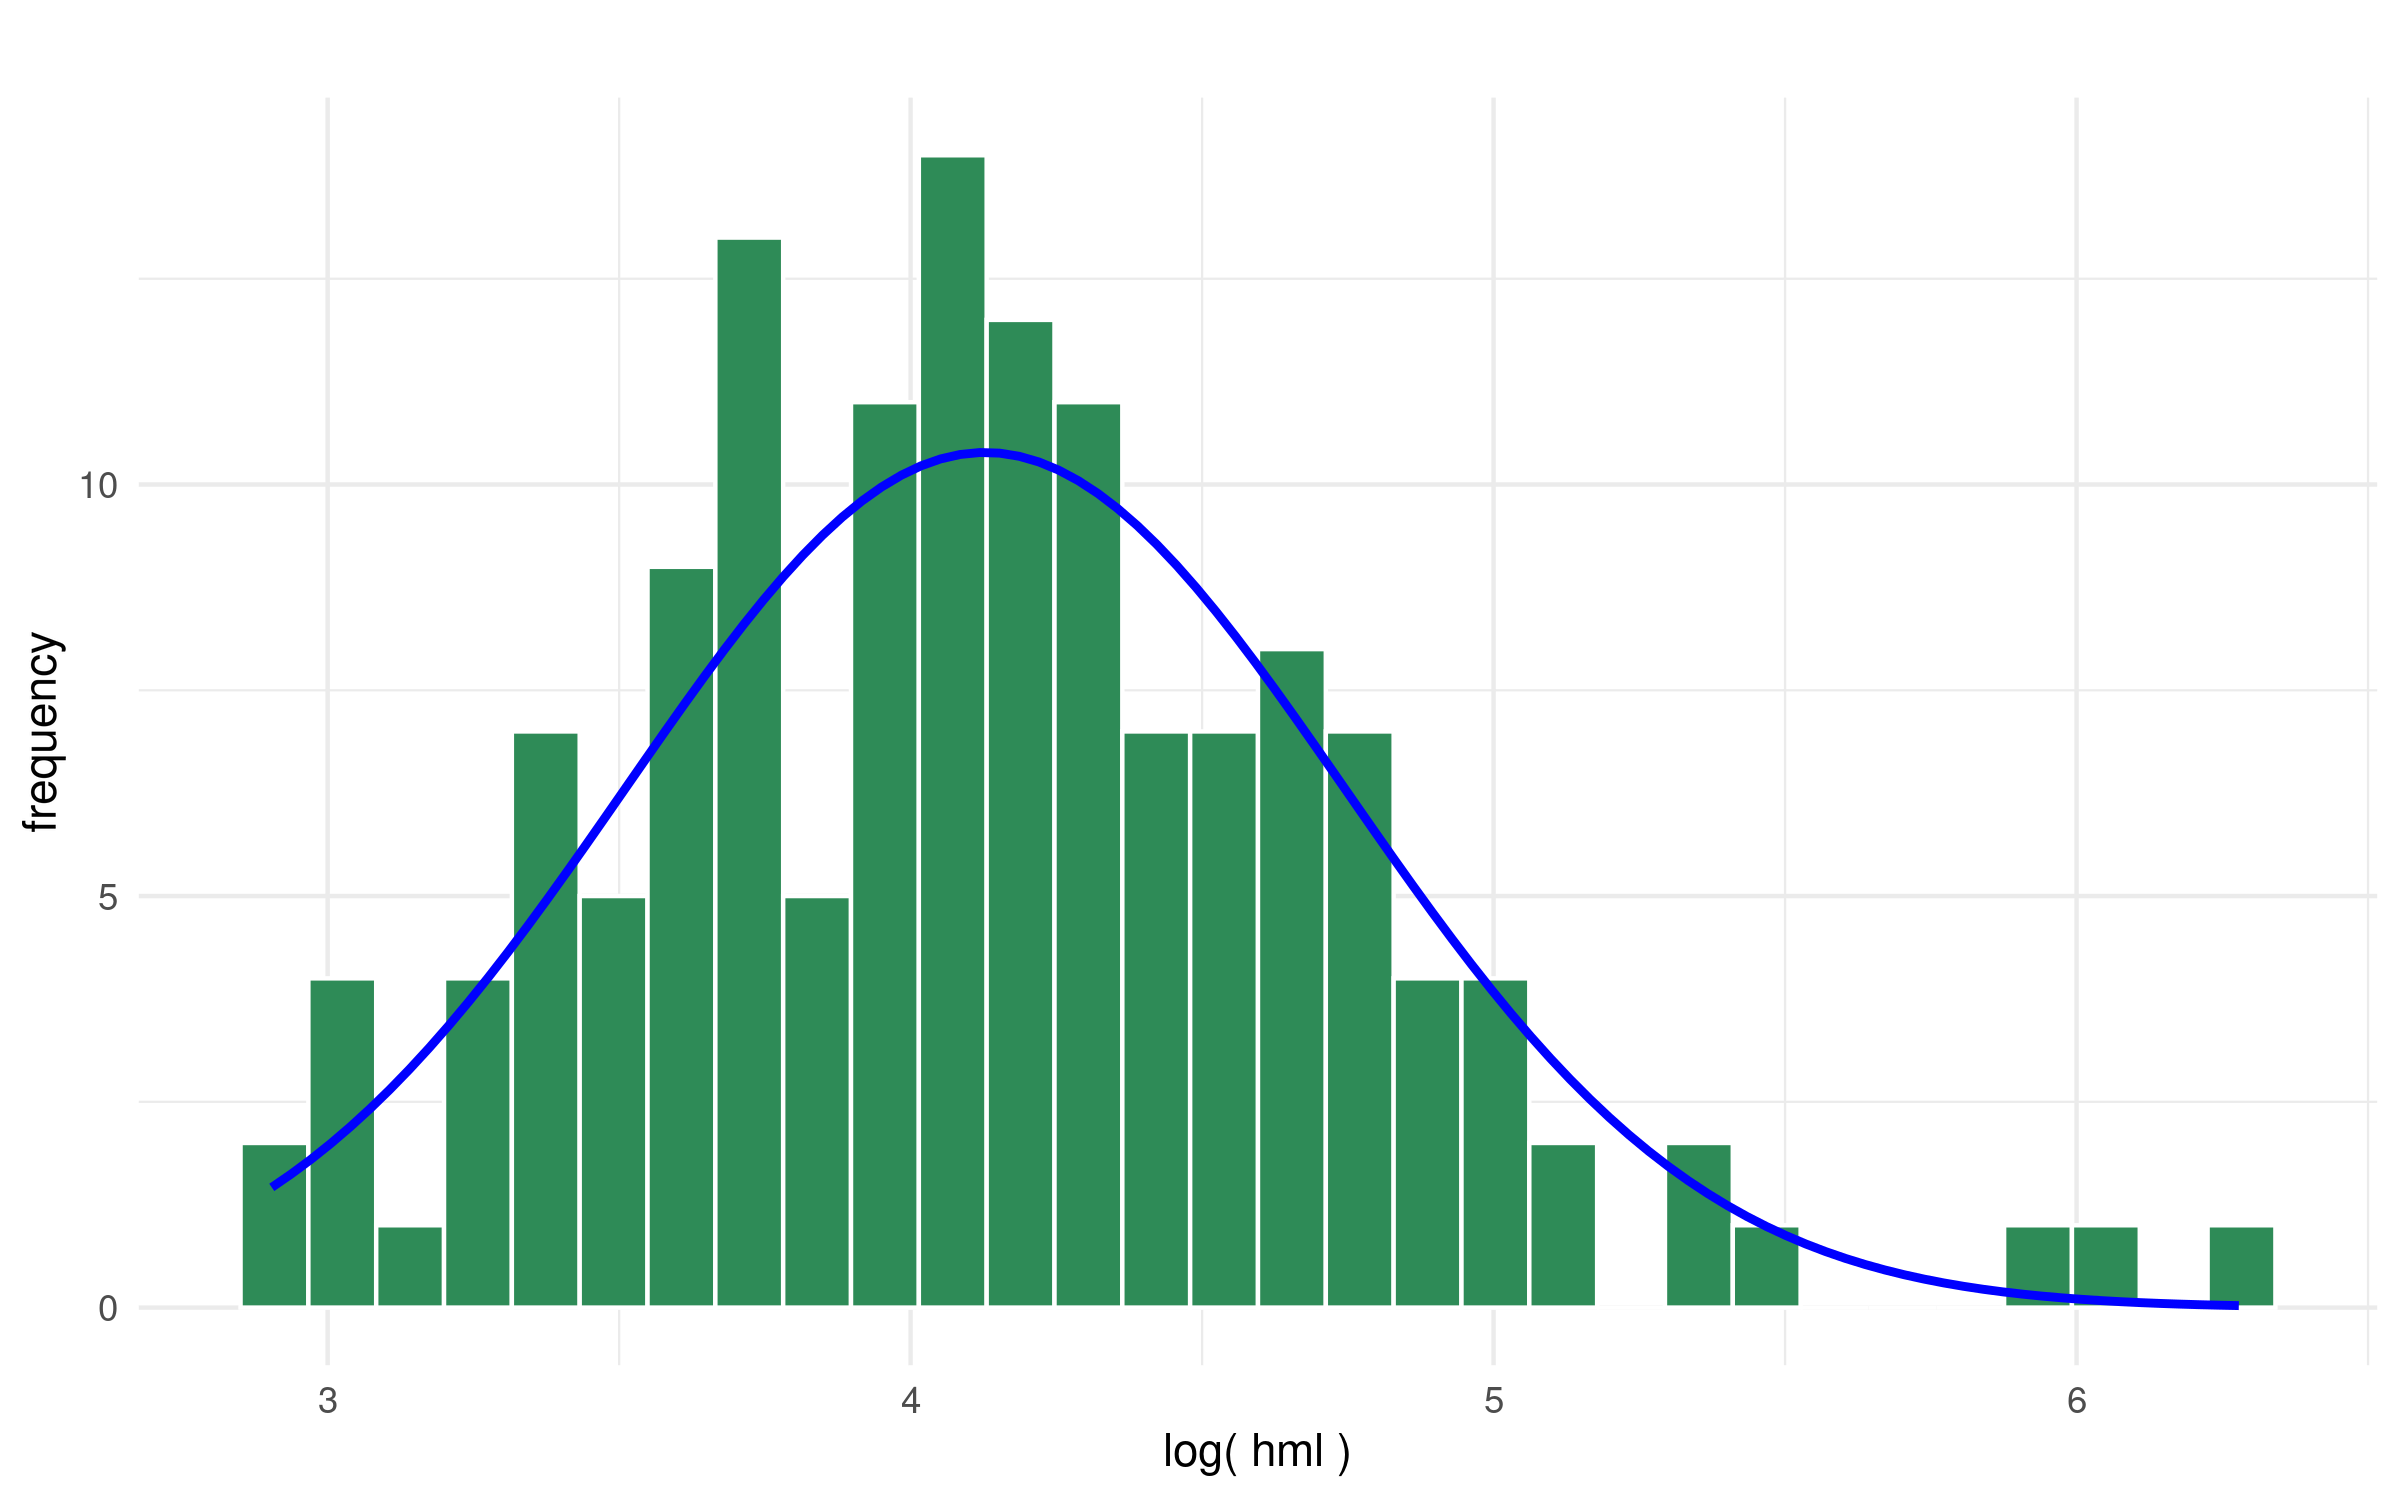
\includegraphics[width=0.7\textwidth]{../pavic_r/hml_loghistogram2.png}
    \caption{Histogram of logarithmic values with the appropriately scaled curve}
    \label{fig:hml_fitted}
\end{figure}

\subsubsection{Volume}

The next quantity we examined was volume. We did not calculate volume because it was provided directly in the table downloaded from Yahoo Finance. As mentioned above, this figure represents the total trading turnover of the S\&P500 index and attempts to account for all ETFs tracking its value. As a result, the figures are enormous, even for the financial sector.

The representation of volume as a time series is:

\begin{figure}[H]
    \centering
    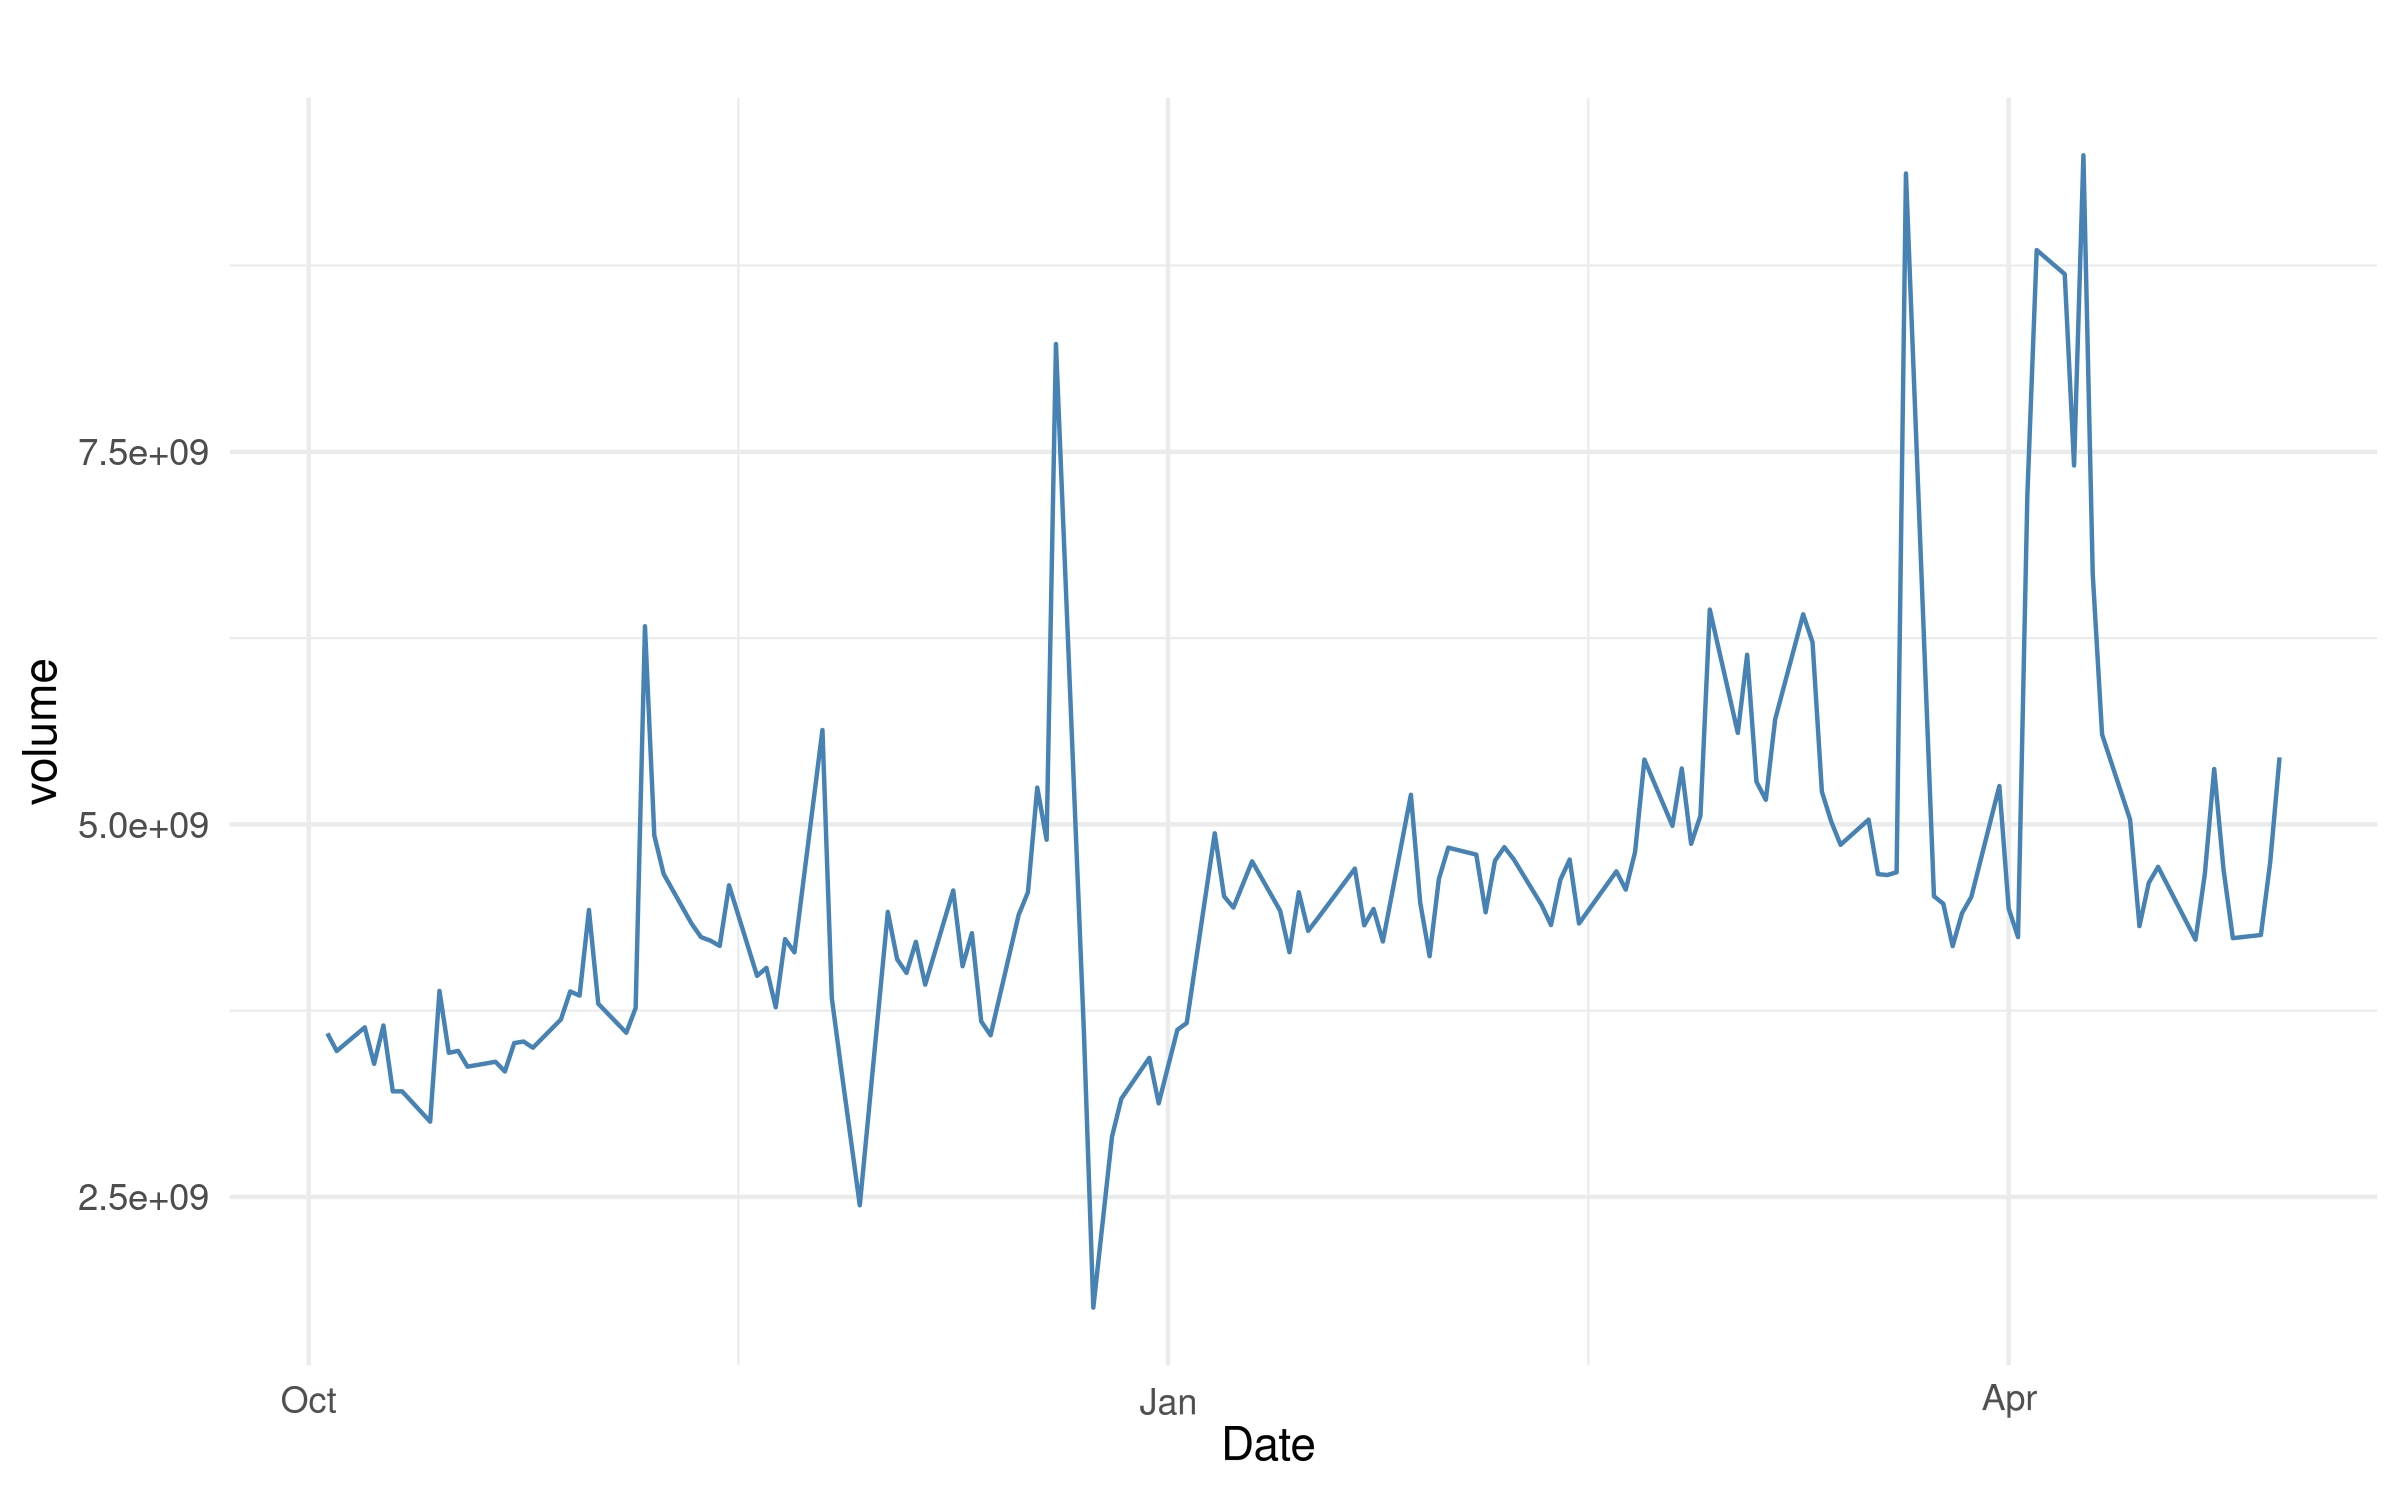
\includegraphics[width=0.8\textwidth]{../pavic_r/volumen_timeseries.png}
    \caption{Volume during the period examined}
    \label{fig:volumen_timeseries}
\end{figure}

The five-number summary is:

\begin{align*}
(x_0(v), q_L(v), m(v), q_U(v), x_{(n)}(v)) &= (1757720000,\; 3880610000,\; 4432250000,\; 4866380000,\; 9489600000)    
\end{align*}

\begin{figure}[H]
    \centering
    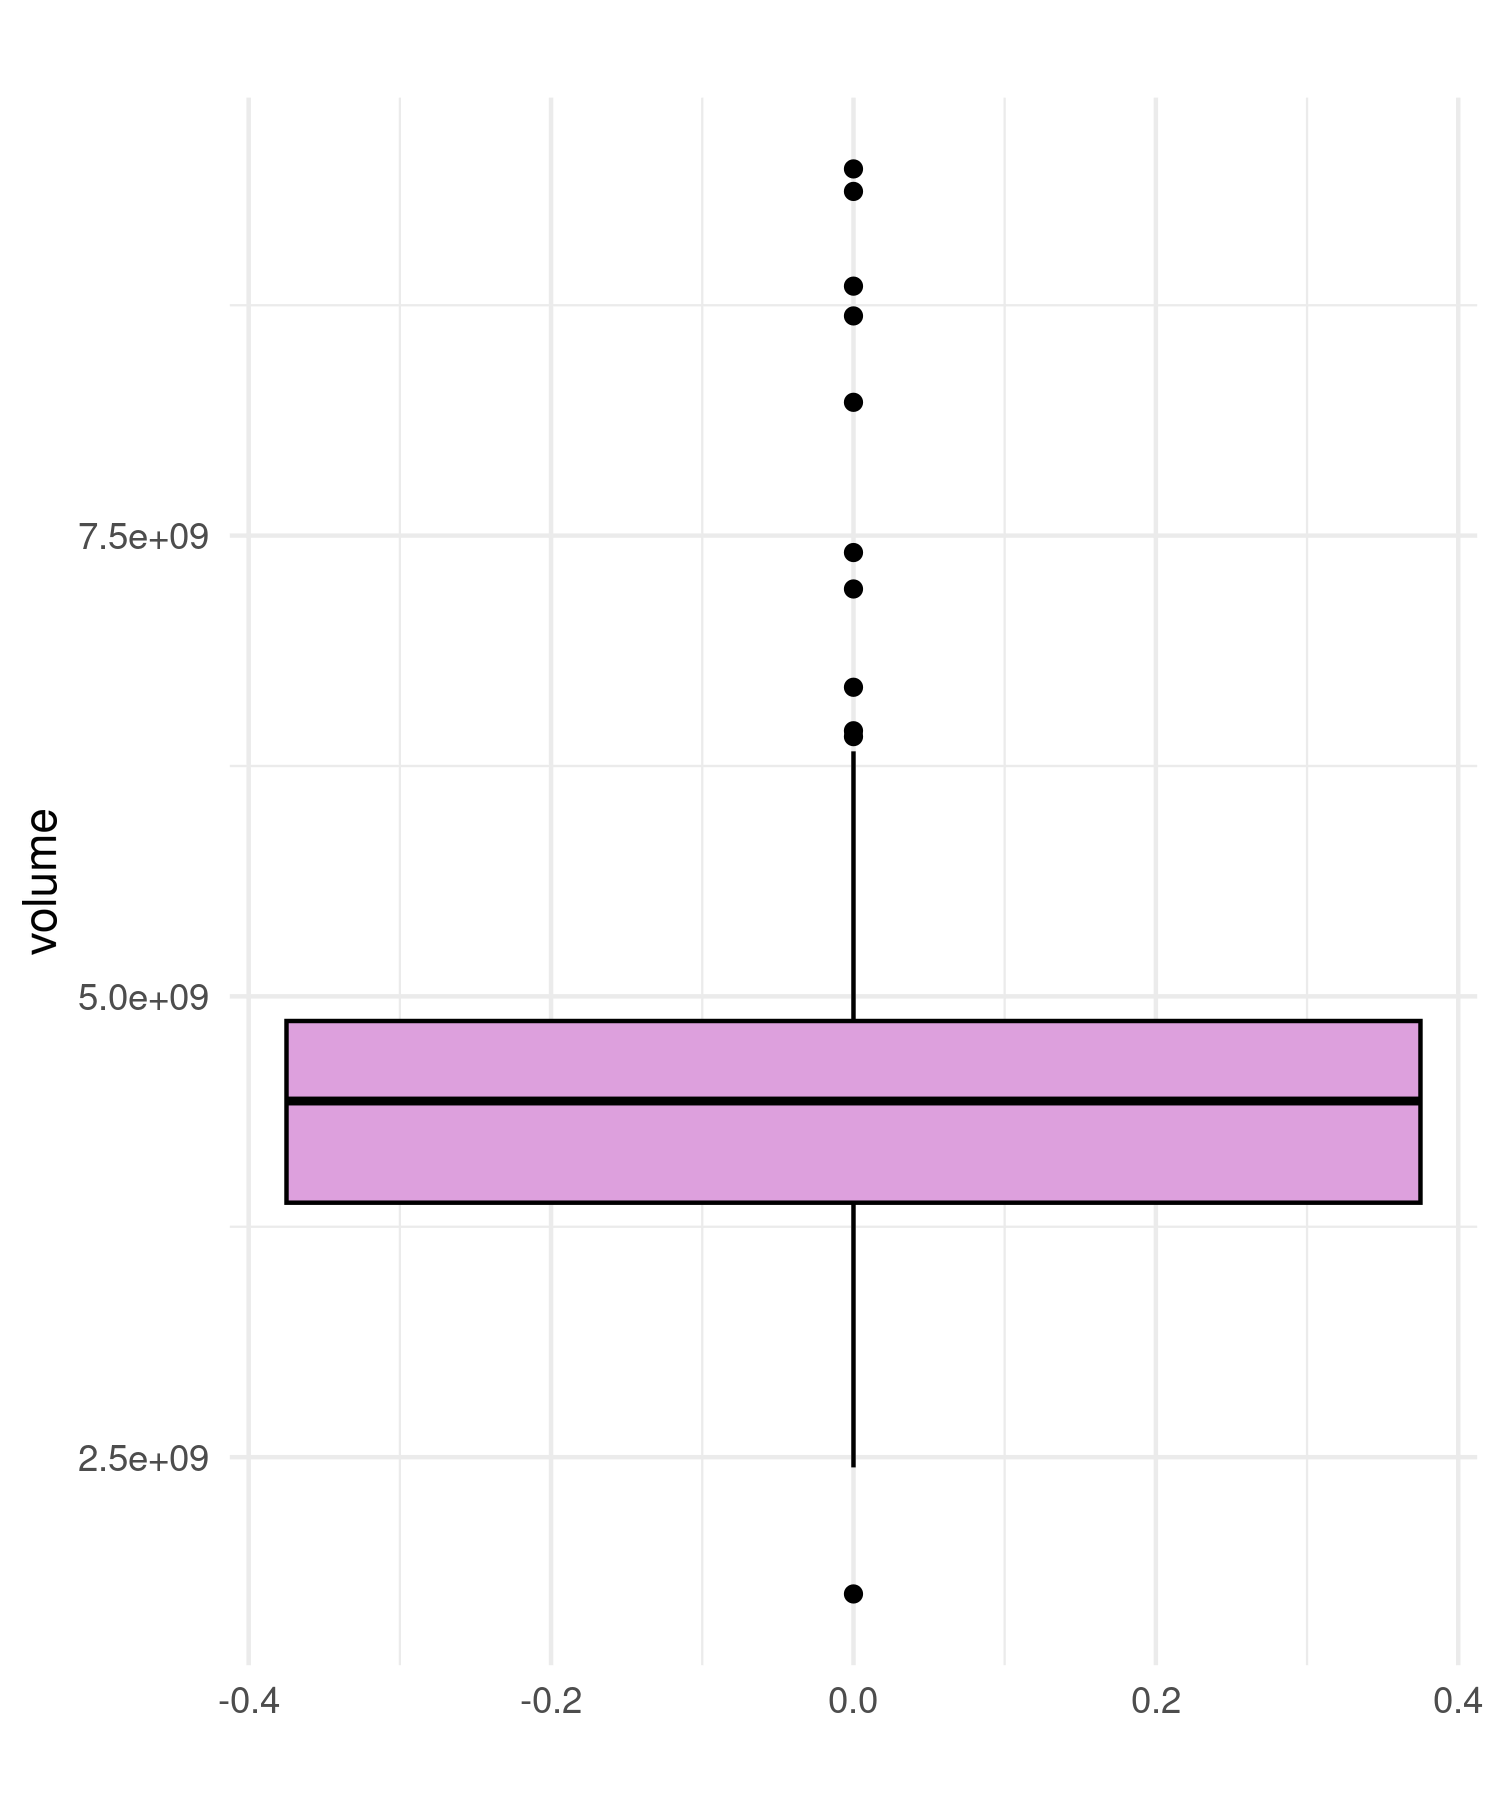
\includegraphics[width=0.4\textwidth]{../pavic_r/volumen_boxplot.png}
    \caption{Boxplot}
    \label{fig:hml_boxplot}
\end{figure}

The boxplot again shows a large number of outliers, for reasons similar to those in the previous example. To obtain a clearer picture of the empirical distribution, we plotted histograms:

\begin{figure}[H]
  \centering
  \begin{subfigure}[b]{0.48\textwidth}
    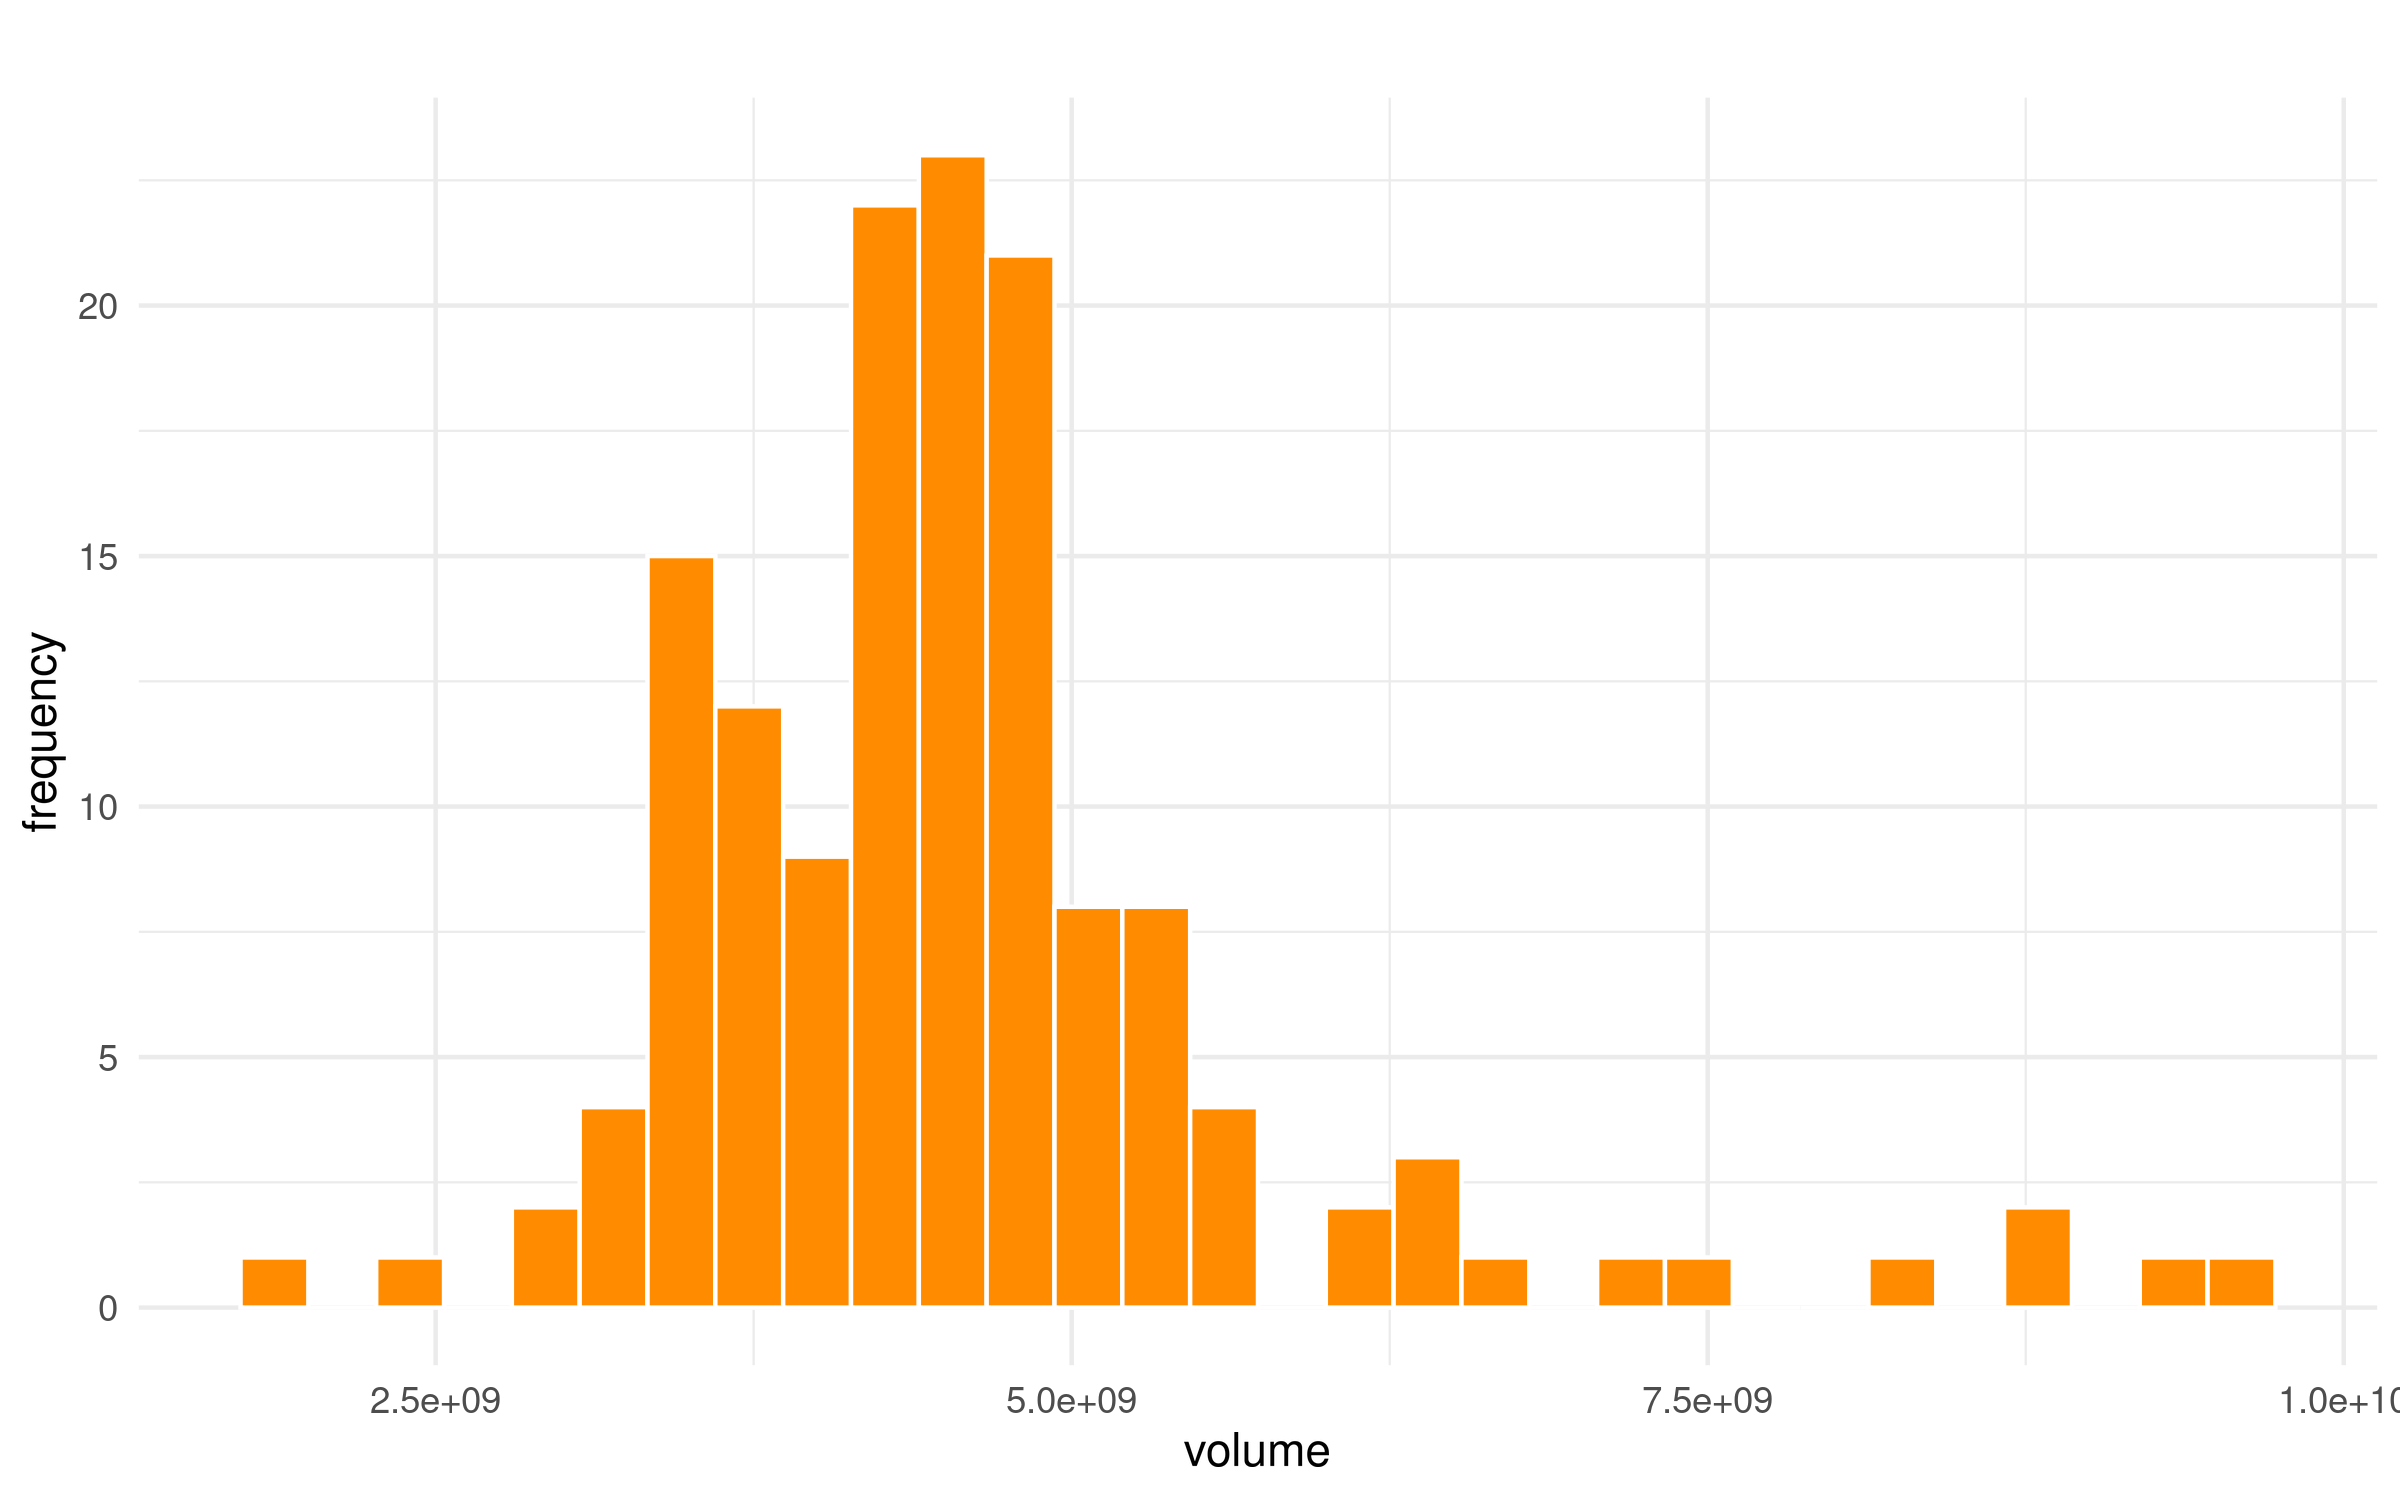
\includegraphics[width=\linewidth]{../pavic_r/volumen_histogram.png}
    \caption{Histogram of volume during the period examined}
    \label{fig:hml_histogram}
  \end{subfigure}
  \hfill
  \begin{subfigure}[b]{0.48\textwidth}
    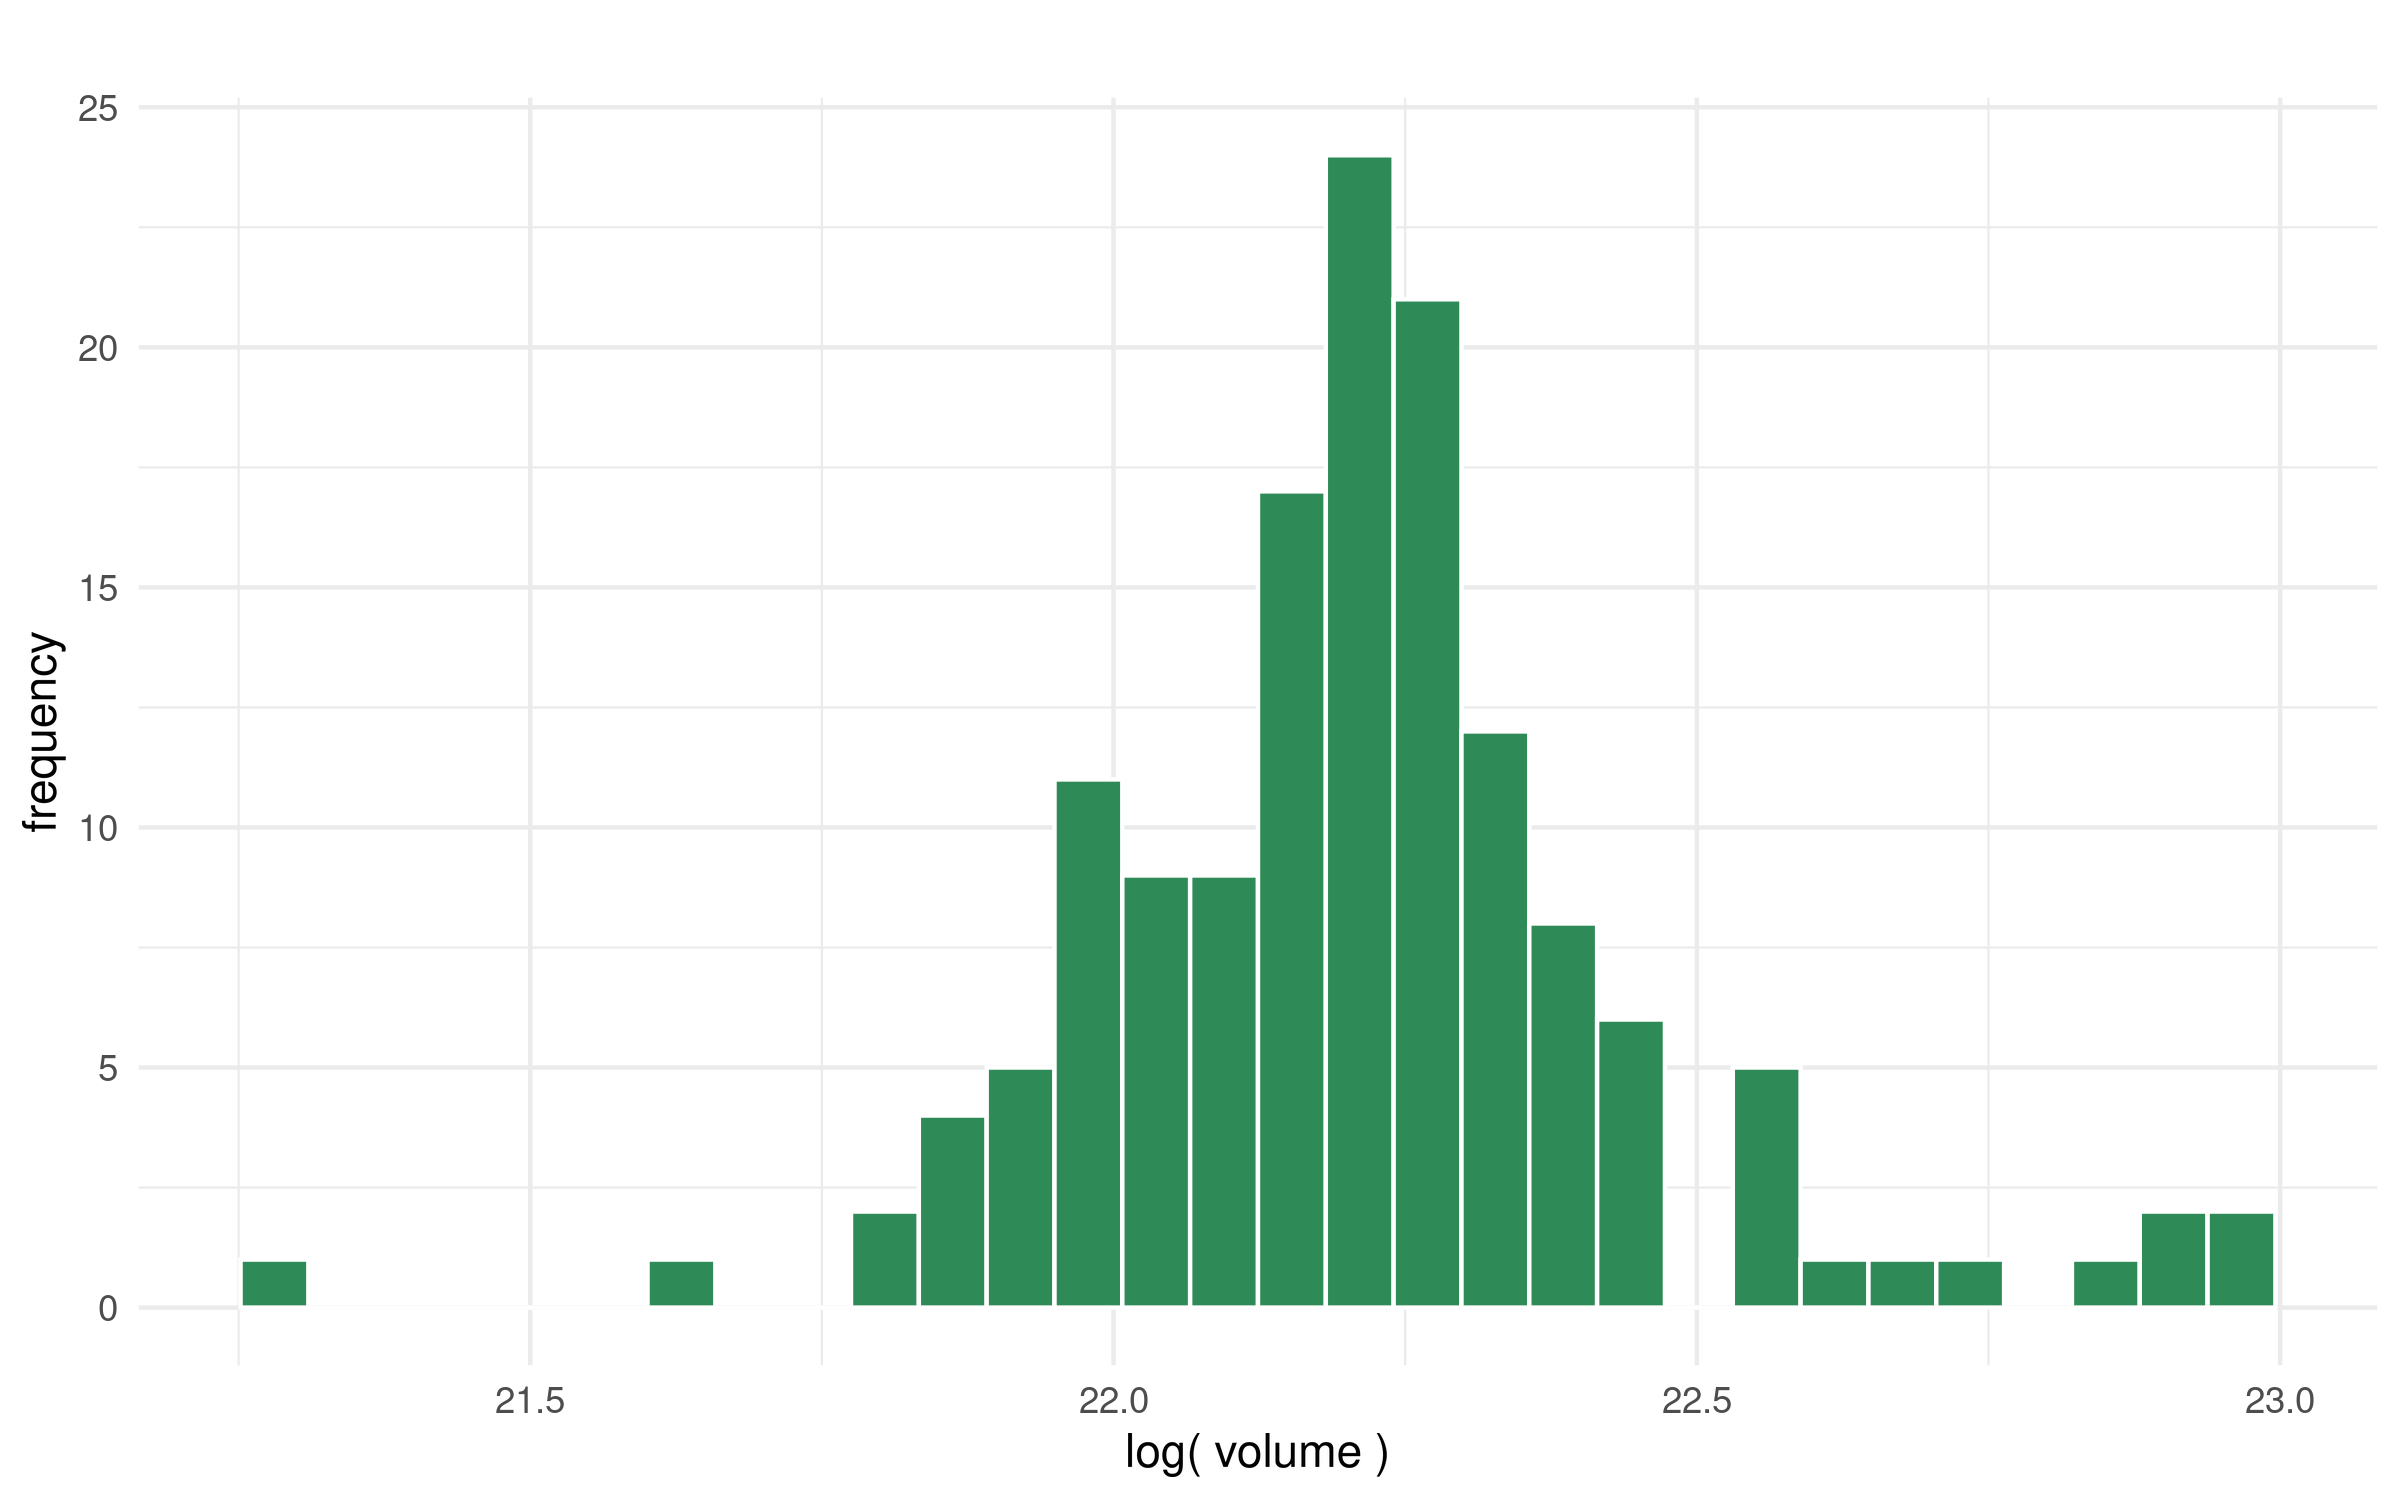
\includegraphics[width=\linewidth]{../pavic_r/volumen_loghistogram.png}
    \caption{Histogram of log(volume) during the period examined}
    \label{fig:hml_loghistogram}
  \end{subfigure}
  \caption{Histograms of volume}
  \label{fig:histograms}
\end{figure}

\subsubsection{Change}

The final quantity we examined is the change between the price at market opening and the price at market closing. We calculated it using the formula

\[ \text{change} = (\,\text{closing price}\,) - (\,\text{opening price}
\,) \]

The representation of change as a time series is:

\begin{figure}[H]
    \centering
    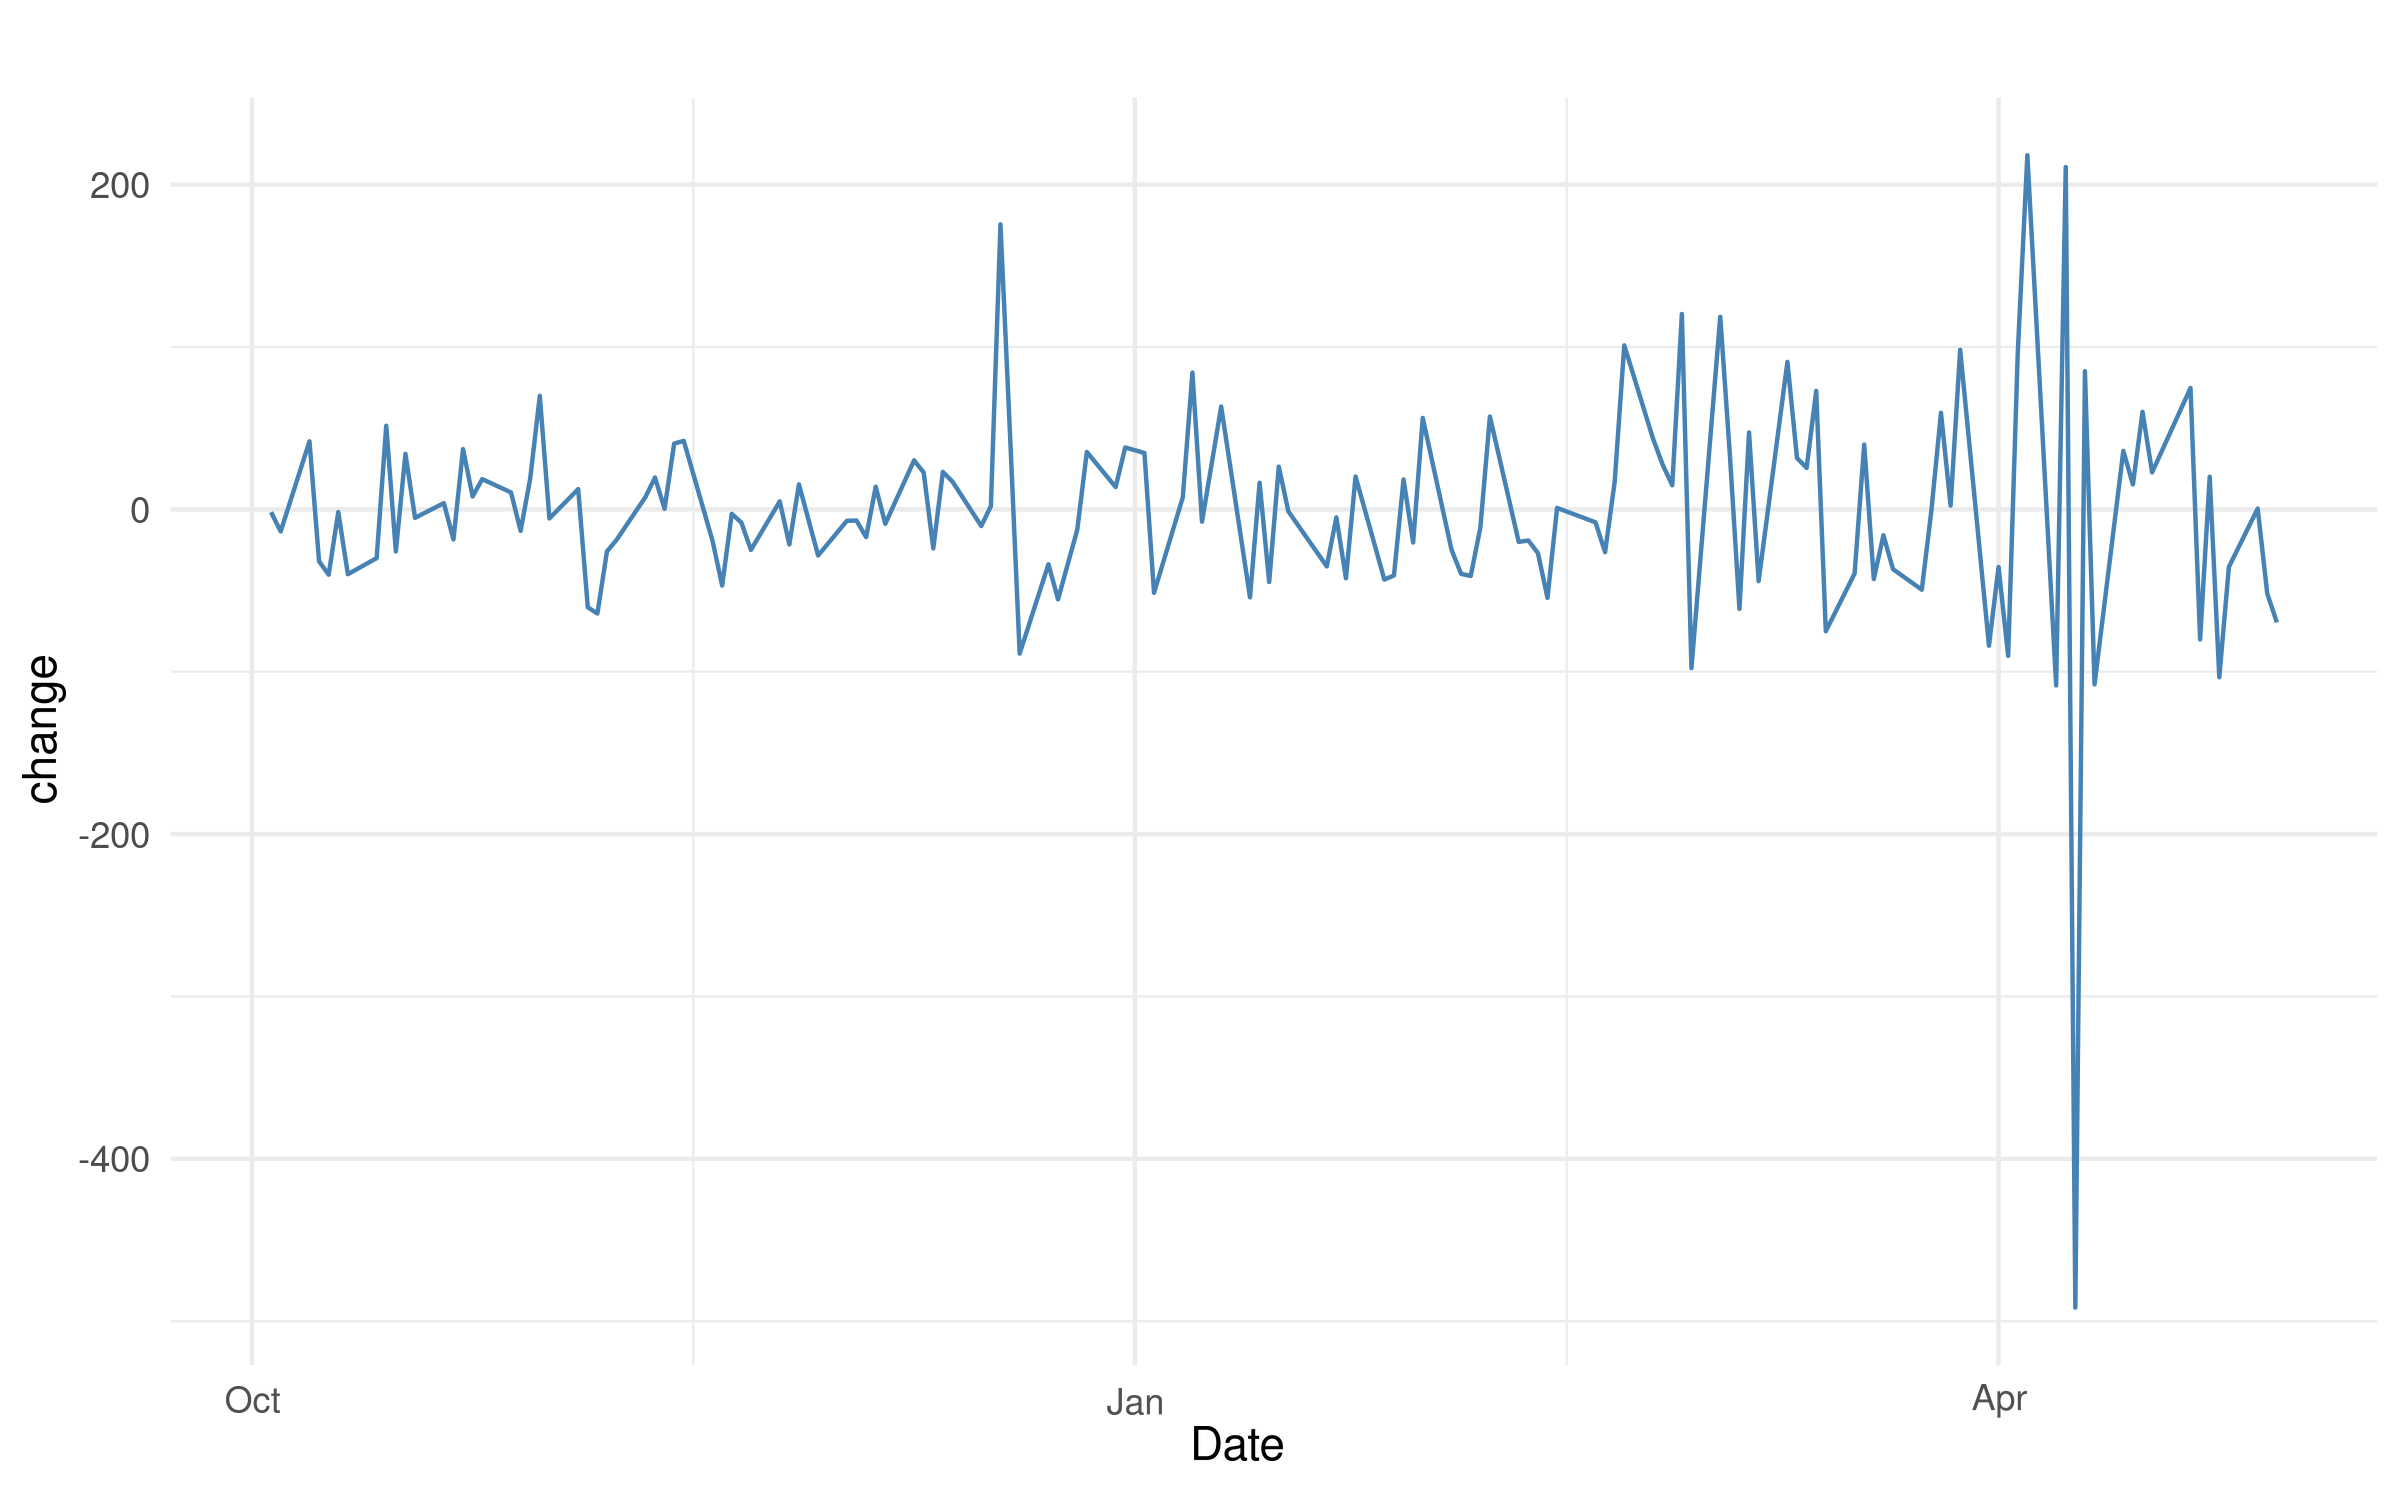
\includegraphics[width=0.8\textwidth]{../pavic_r/promjena_timeseries.png}
    \caption{Change during the period examined}
    \label{fig:volatilnost_timeseries}
\end{figure}

The five-number summary is:

\begin{align*}
(x_0(v), q_L(v), m(v), q_U(v), x_{(n)}(v)) &= (-491.62012,\; -34.46997,\; -1.75000,\; 28.81982,\; 218.06006)    
\end{align*}

\begin{figure}[H]
    \centering
    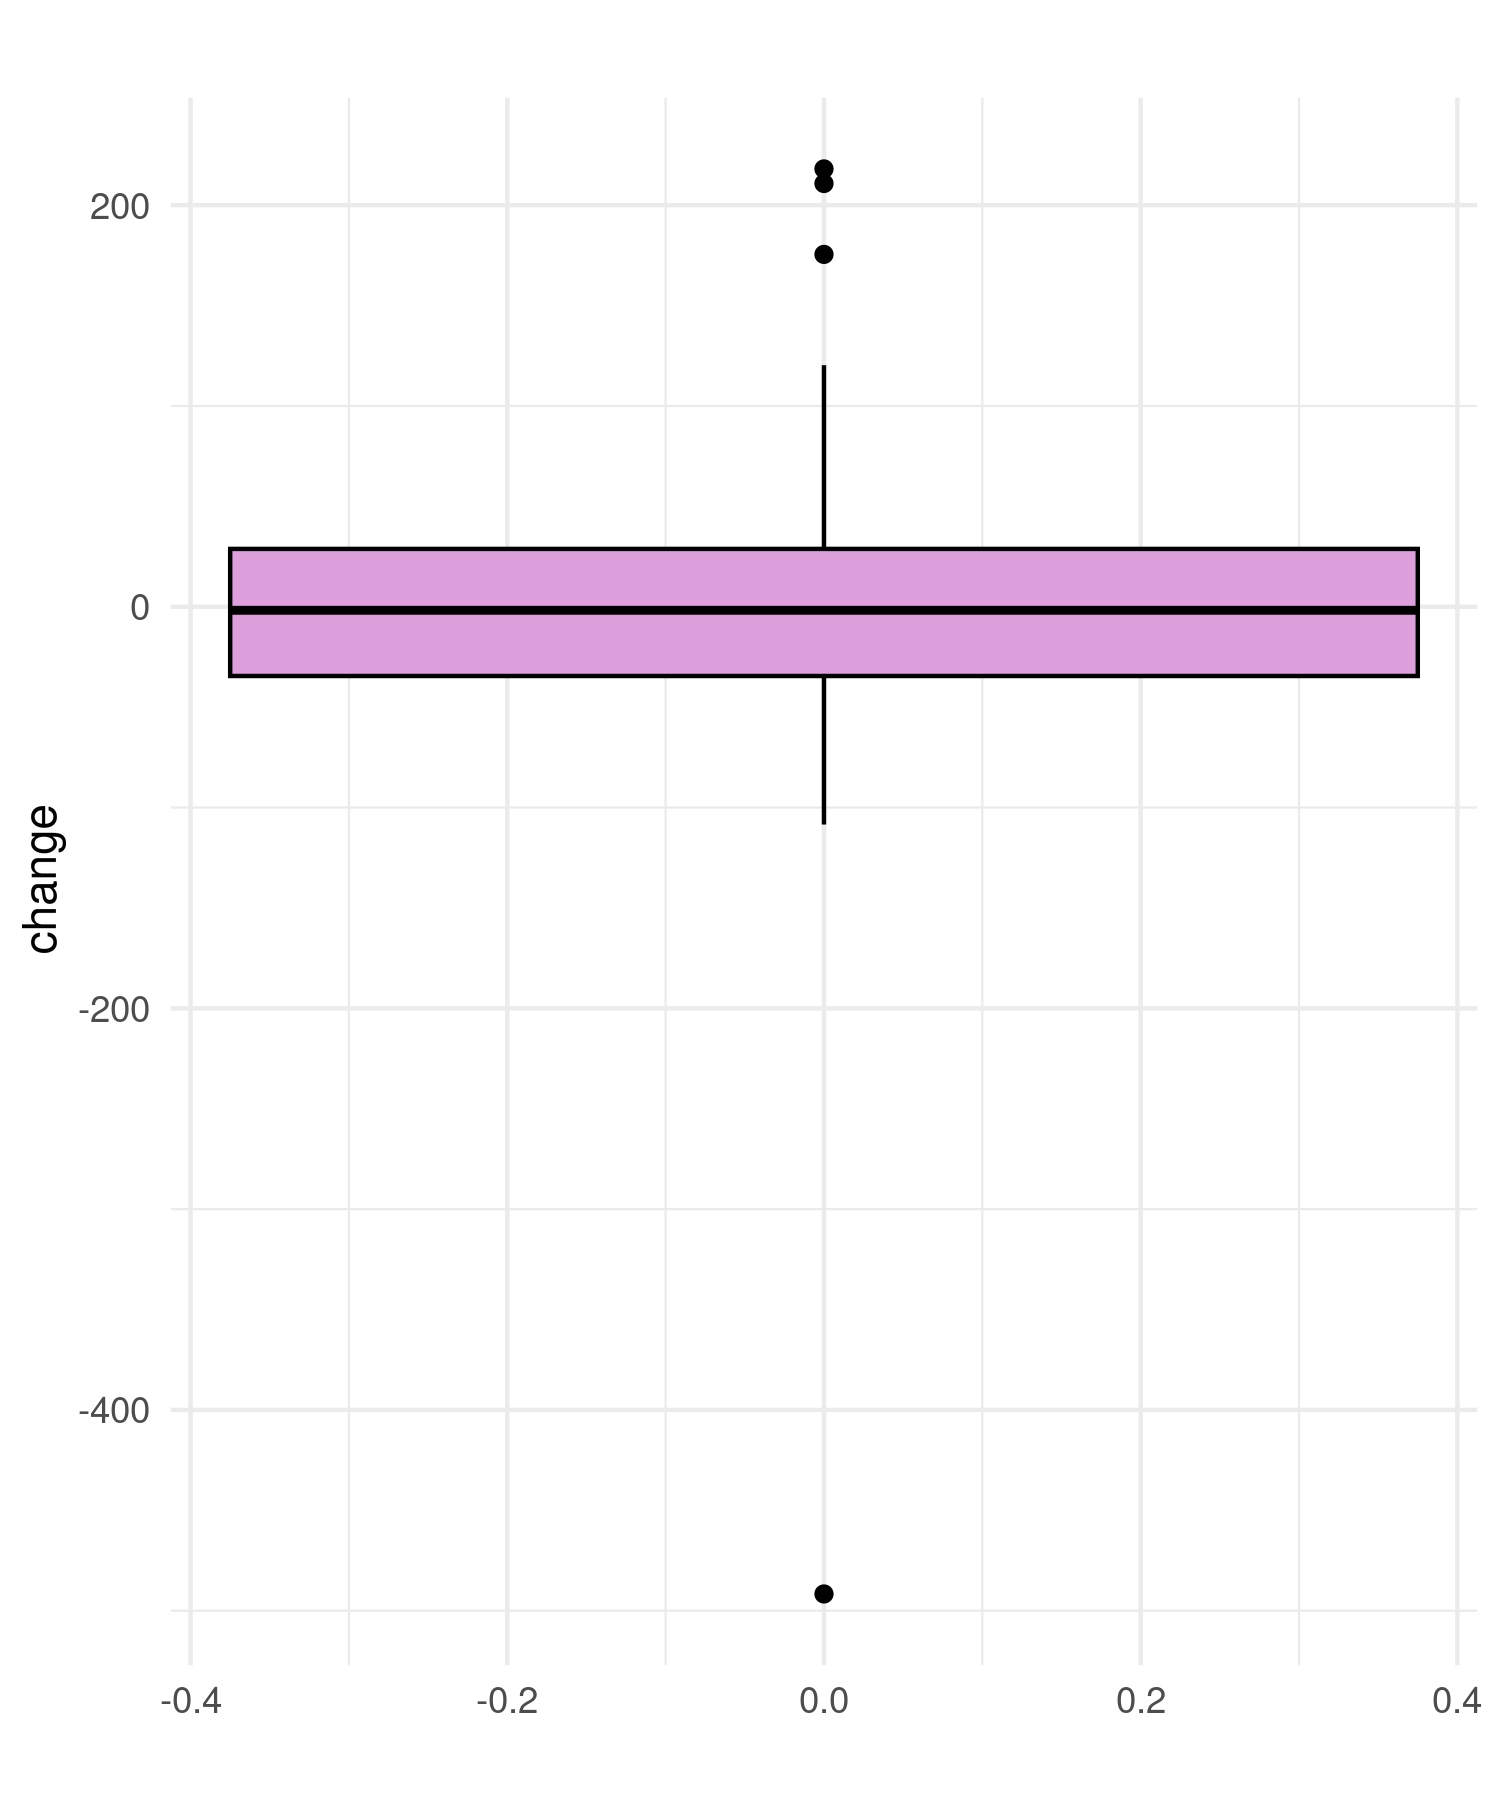
\includegraphics[width=0.4\textwidth]{../pavic_r/promjena_boxplot.png}
    \caption{Boxplot}
    \label{fig:hml_boxplot}
\end{figure}

Because of the large outlier corresponding exactly to the day tariffs were introduced, we decided to plot not only the ordinary histogram but also a histogram of the data from the $5$th to the $95$th percentile, to see the distribution of the central data more clearly.

\begin{figure}[H]
  \centering
  \begin{subfigure}[b]{0.48\textwidth}
    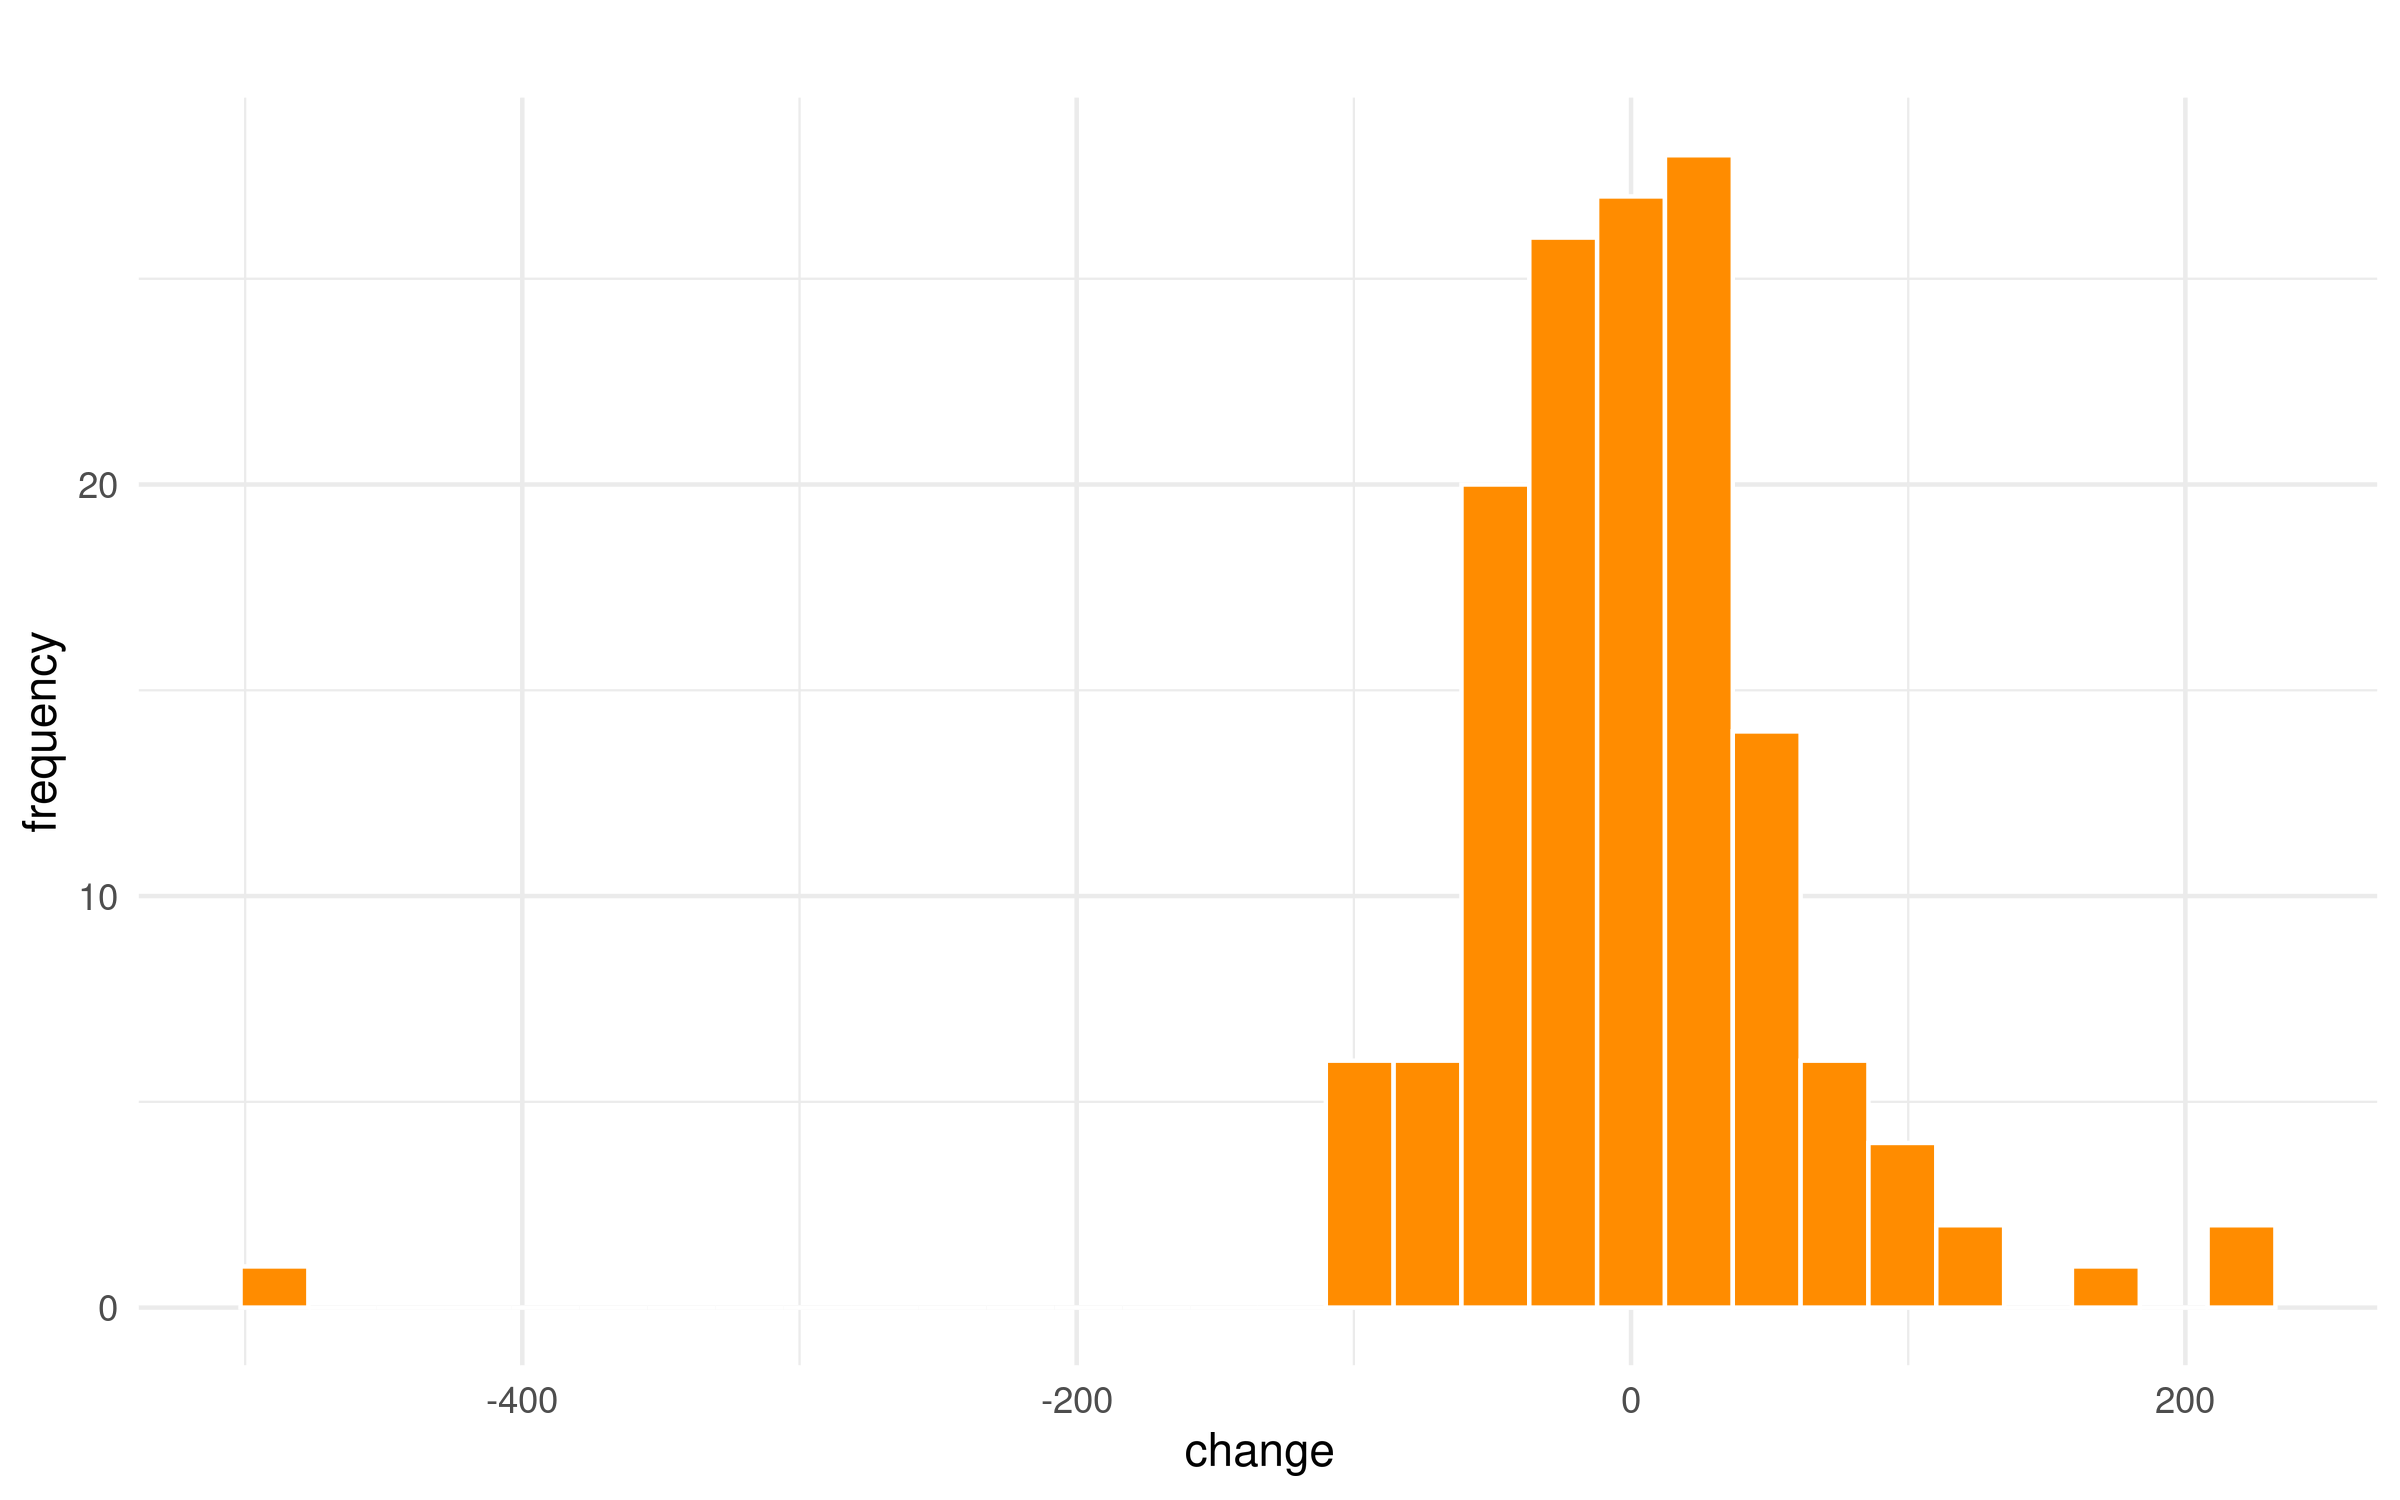
\includegraphics[width=\linewidth]{../pavic_r/promjena_histogram.png}
    \caption{Histogram of volume during the period examined}
    \label{fig:hml_histogram}
  \end{subfigure}
  \hfill
  \begin{subfigure}[b]{0.48\textwidth}
    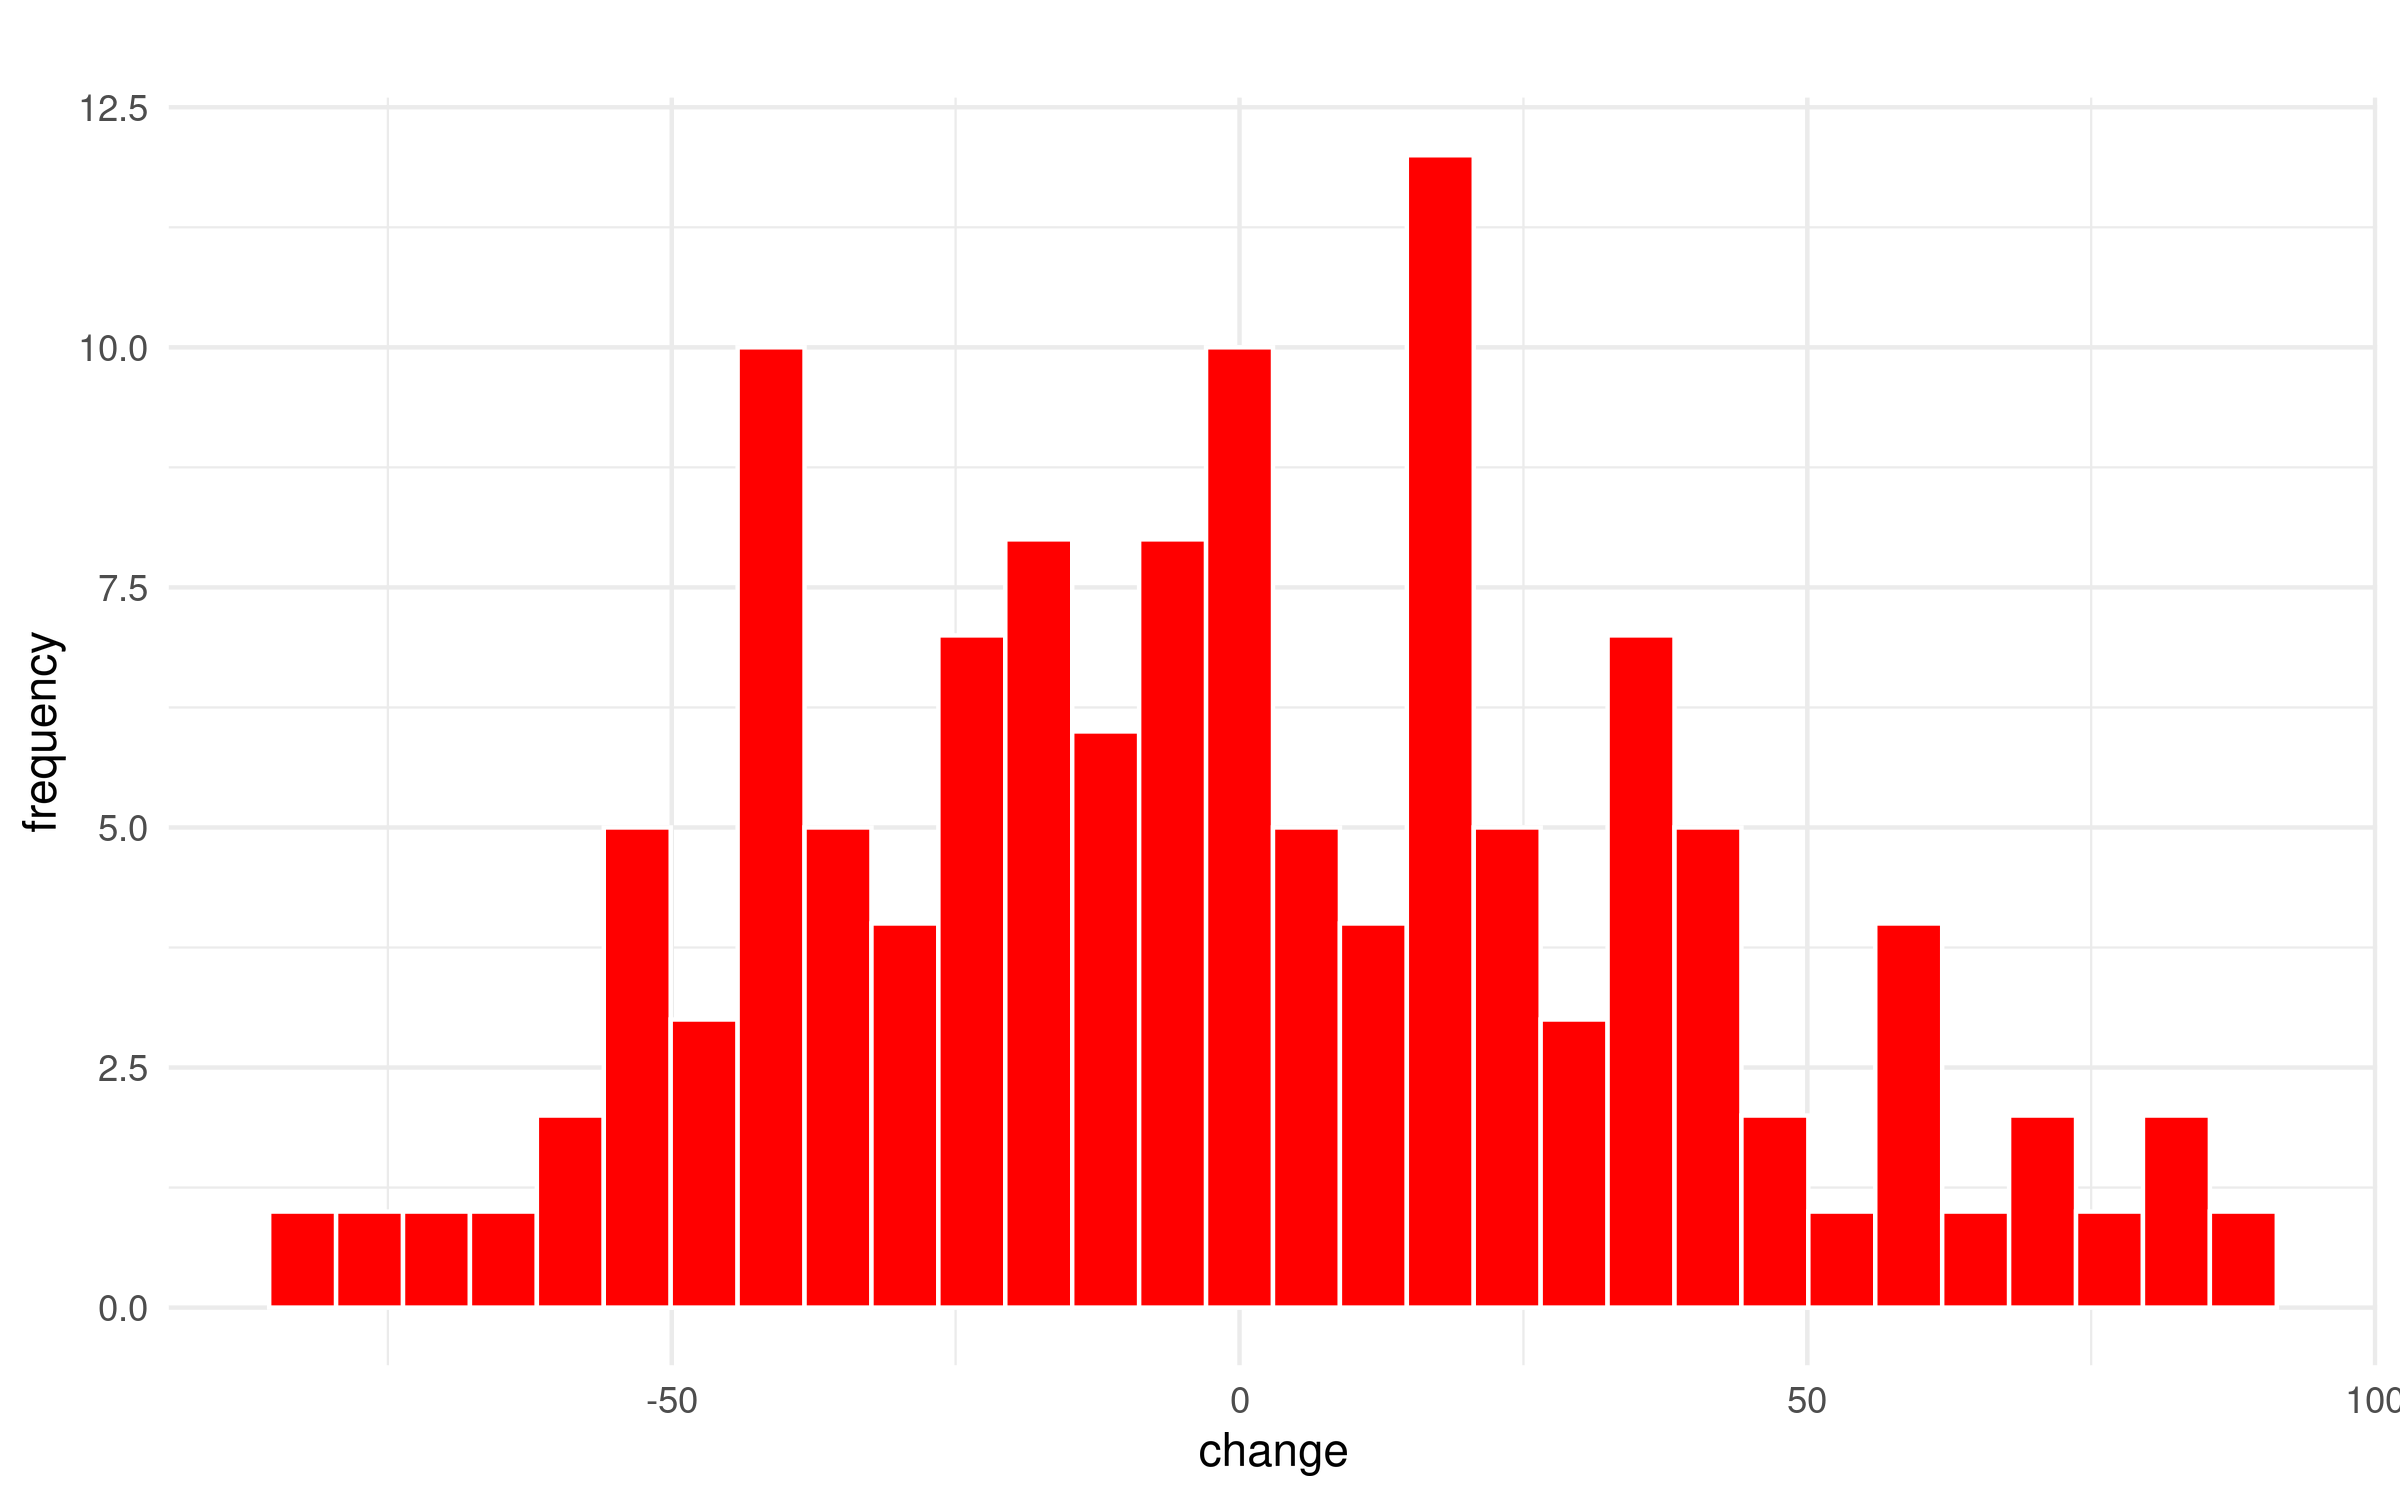
\includegraphics[width=\linewidth]{../pavic_r/promjena_filtrirani_histogram.png}
    \caption{Filtered histogram of volume during the period examined}
    \label{fig:hml_loghistogram}
  \end{subfigure}
  \caption{Histograms of volume}
  \label{fig:histograms}
\end{figure}

Based on the histogram, we decided to test whether change is normally distributed.
Specifically, we performed a test for the MLE given by the parameters

\[ \hat{\mu} = -0.9113 \;\; \hat{\sigma}^2 = 4675.9851 \]

The distribution is shown below, overlaid with the theoretical curve:

\begin{figure}[H]
    \centering
    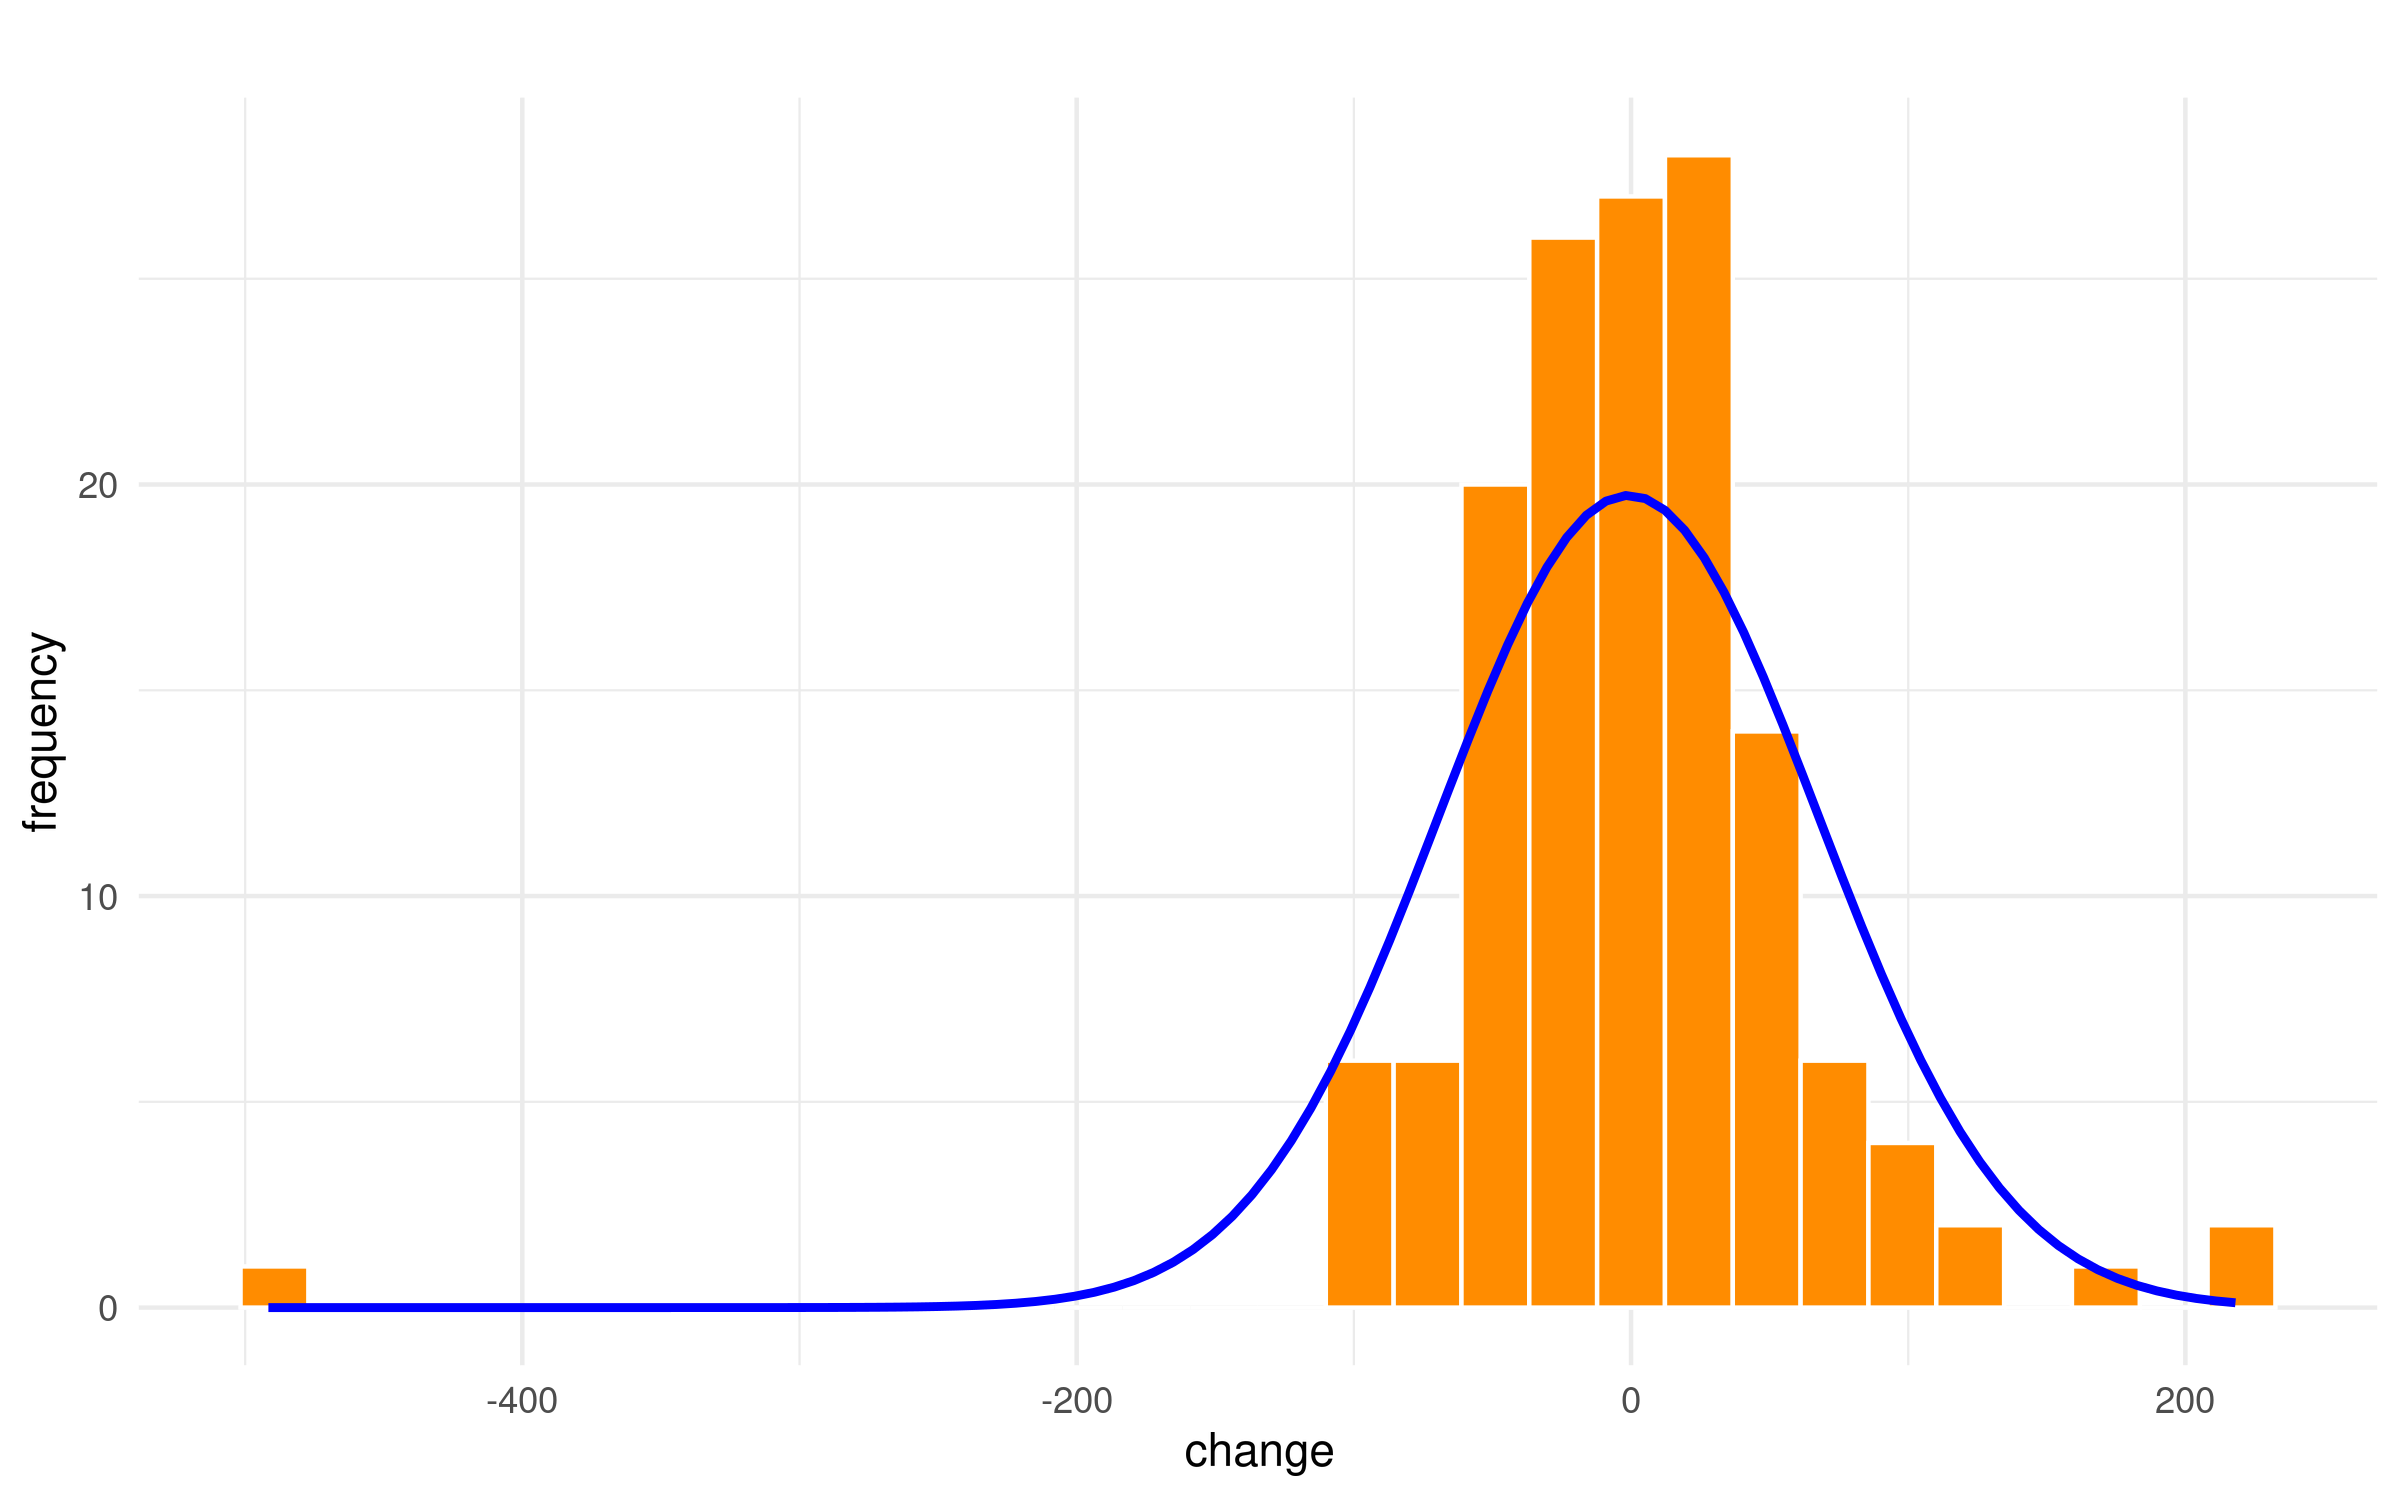
\includegraphics[width=0.7\textwidth]{../pavic_r/promjena_histogram2.png}
    \caption{Histogram with the appropriately scaled curve}
    \label{fig:promjena_fitted}
\end{figure}

\newpage
\subsection{Search data}

The data shown throughout represent \textbf{relative} frequencies: each frequency is divided by the highest frequency in the given time interval and multiplied by $100$. The maximum value in both time series will therefore be exactly $100$.

The data represented as time series are:

\begin{figure}[H]
  \centering
  \begin{subfigure}[b]{0.48\textwidth}
    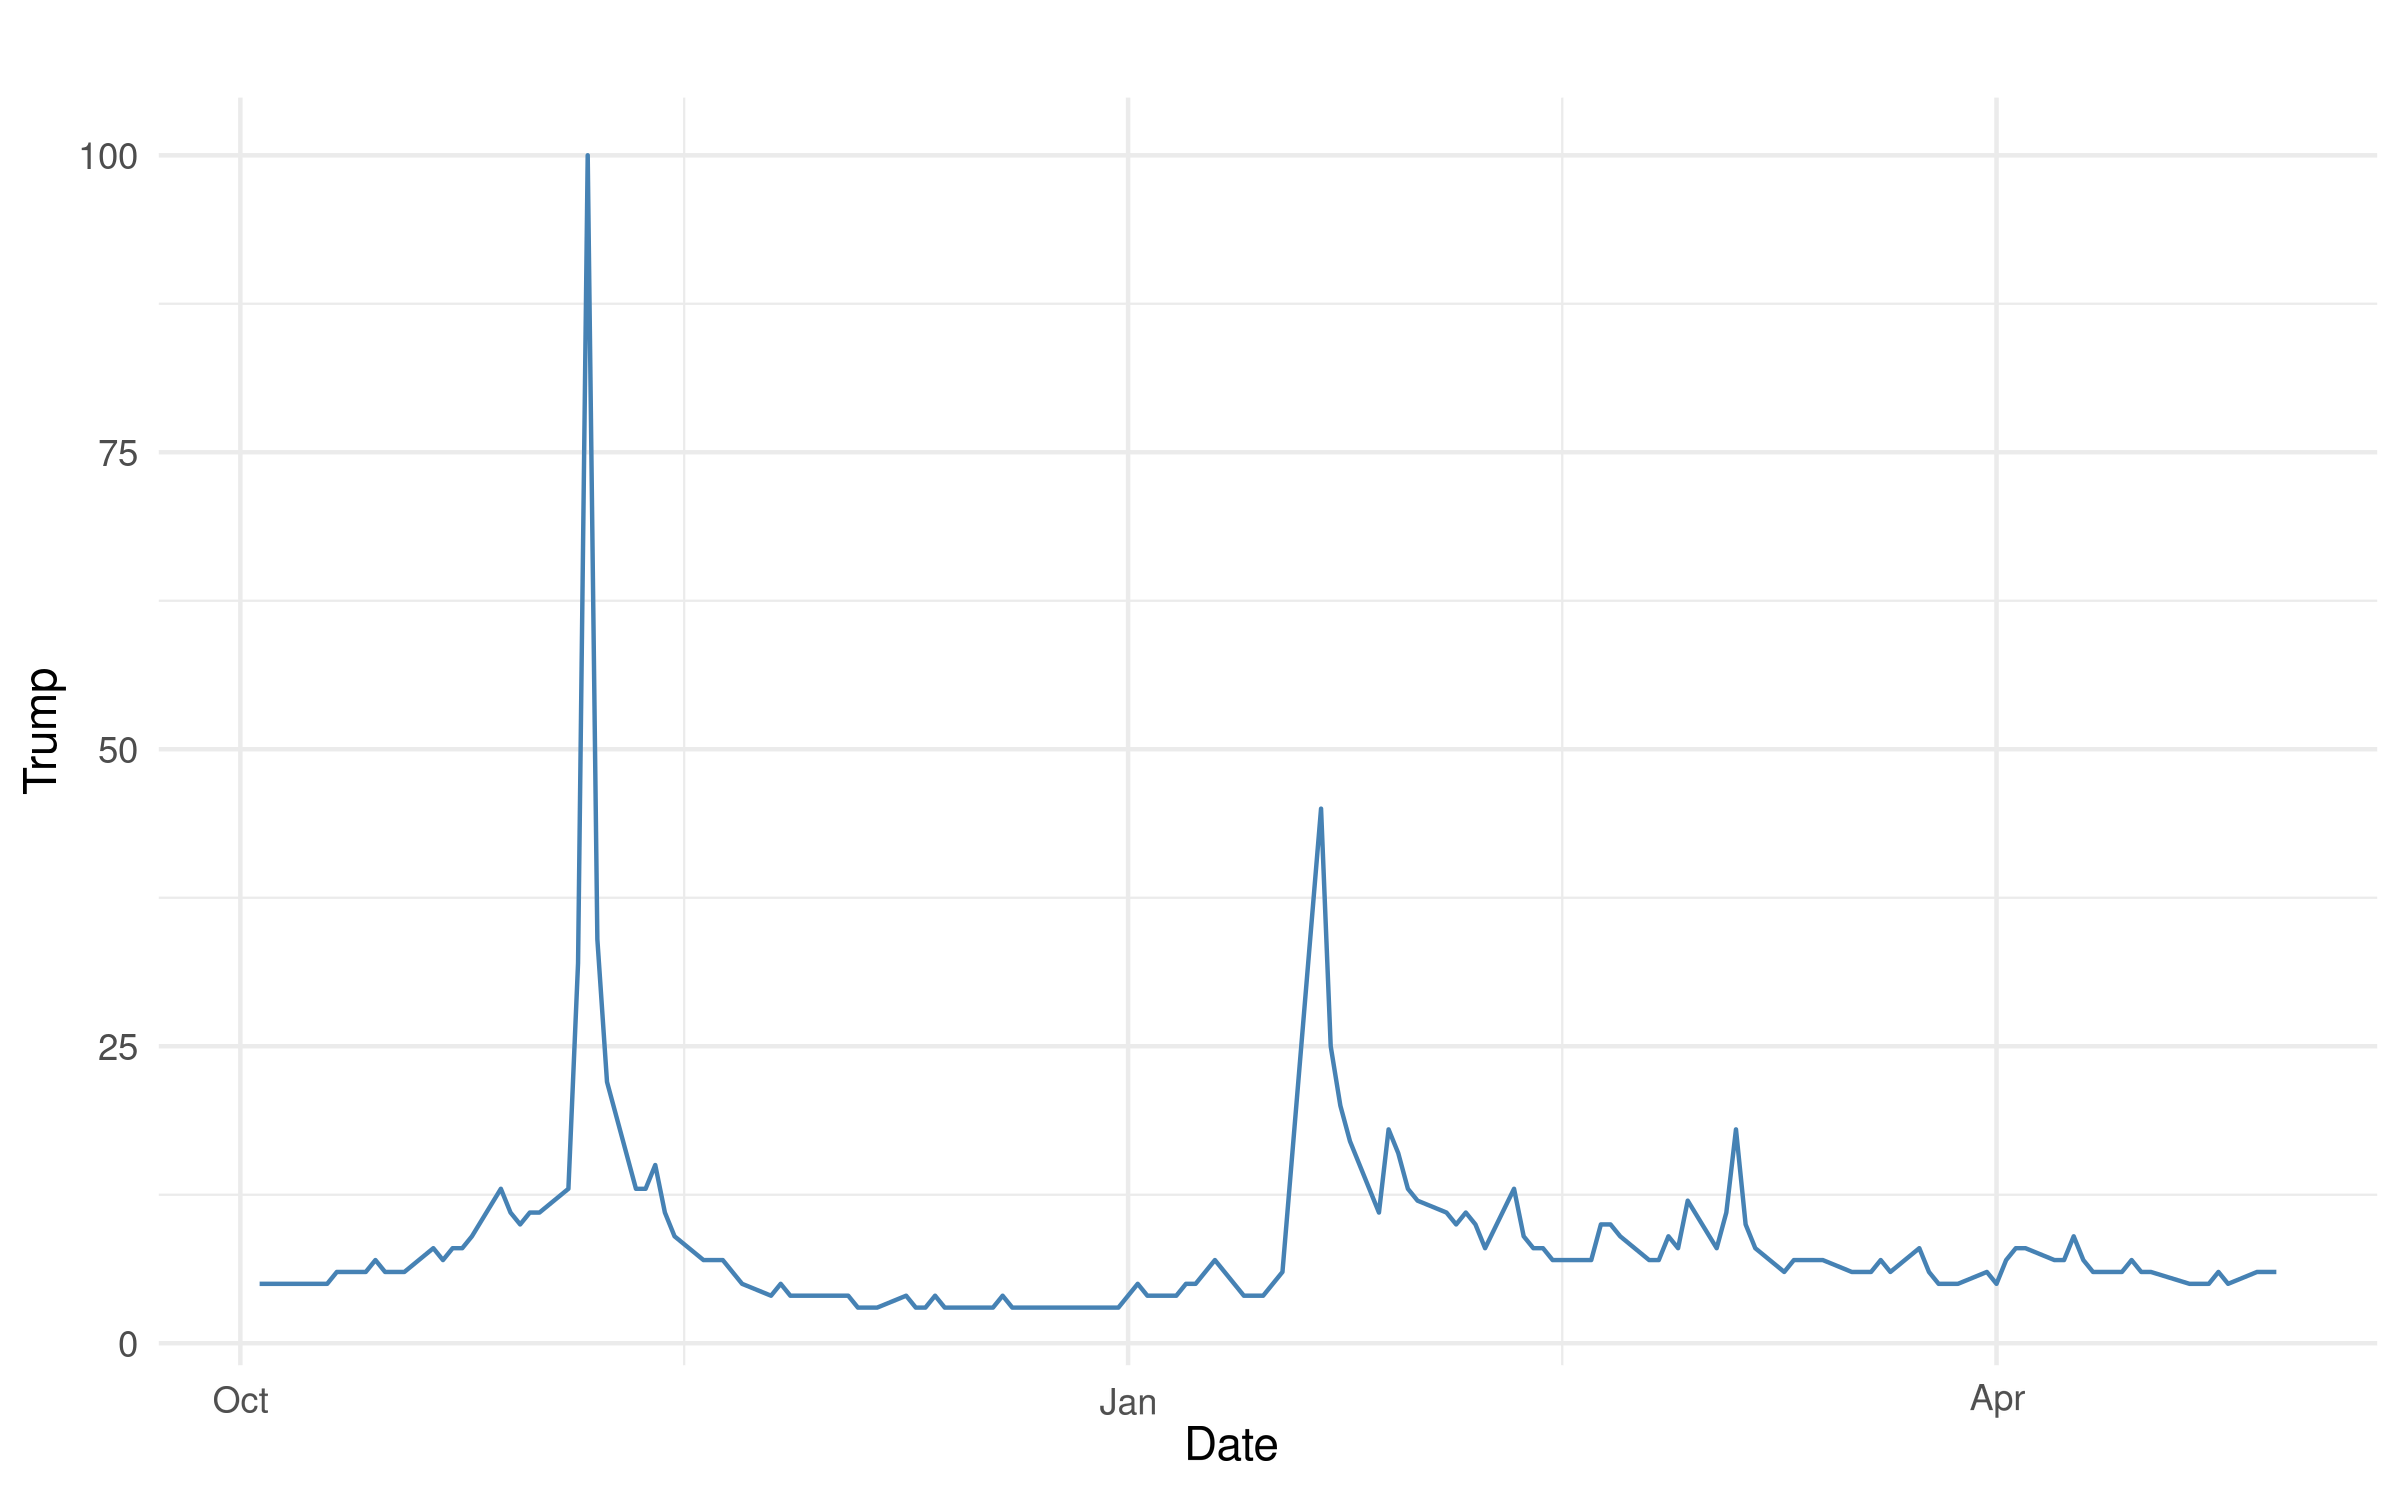
\includegraphics[width=\linewidth]{../pavic_r/Trump_timeseries.png}
    \caption{The term "Trump"}
    \label{fig:trump_timeseries}
  \end{subfigure}
  \hfill
  \begin{subfigure}[b]{0.48\textwidth}
    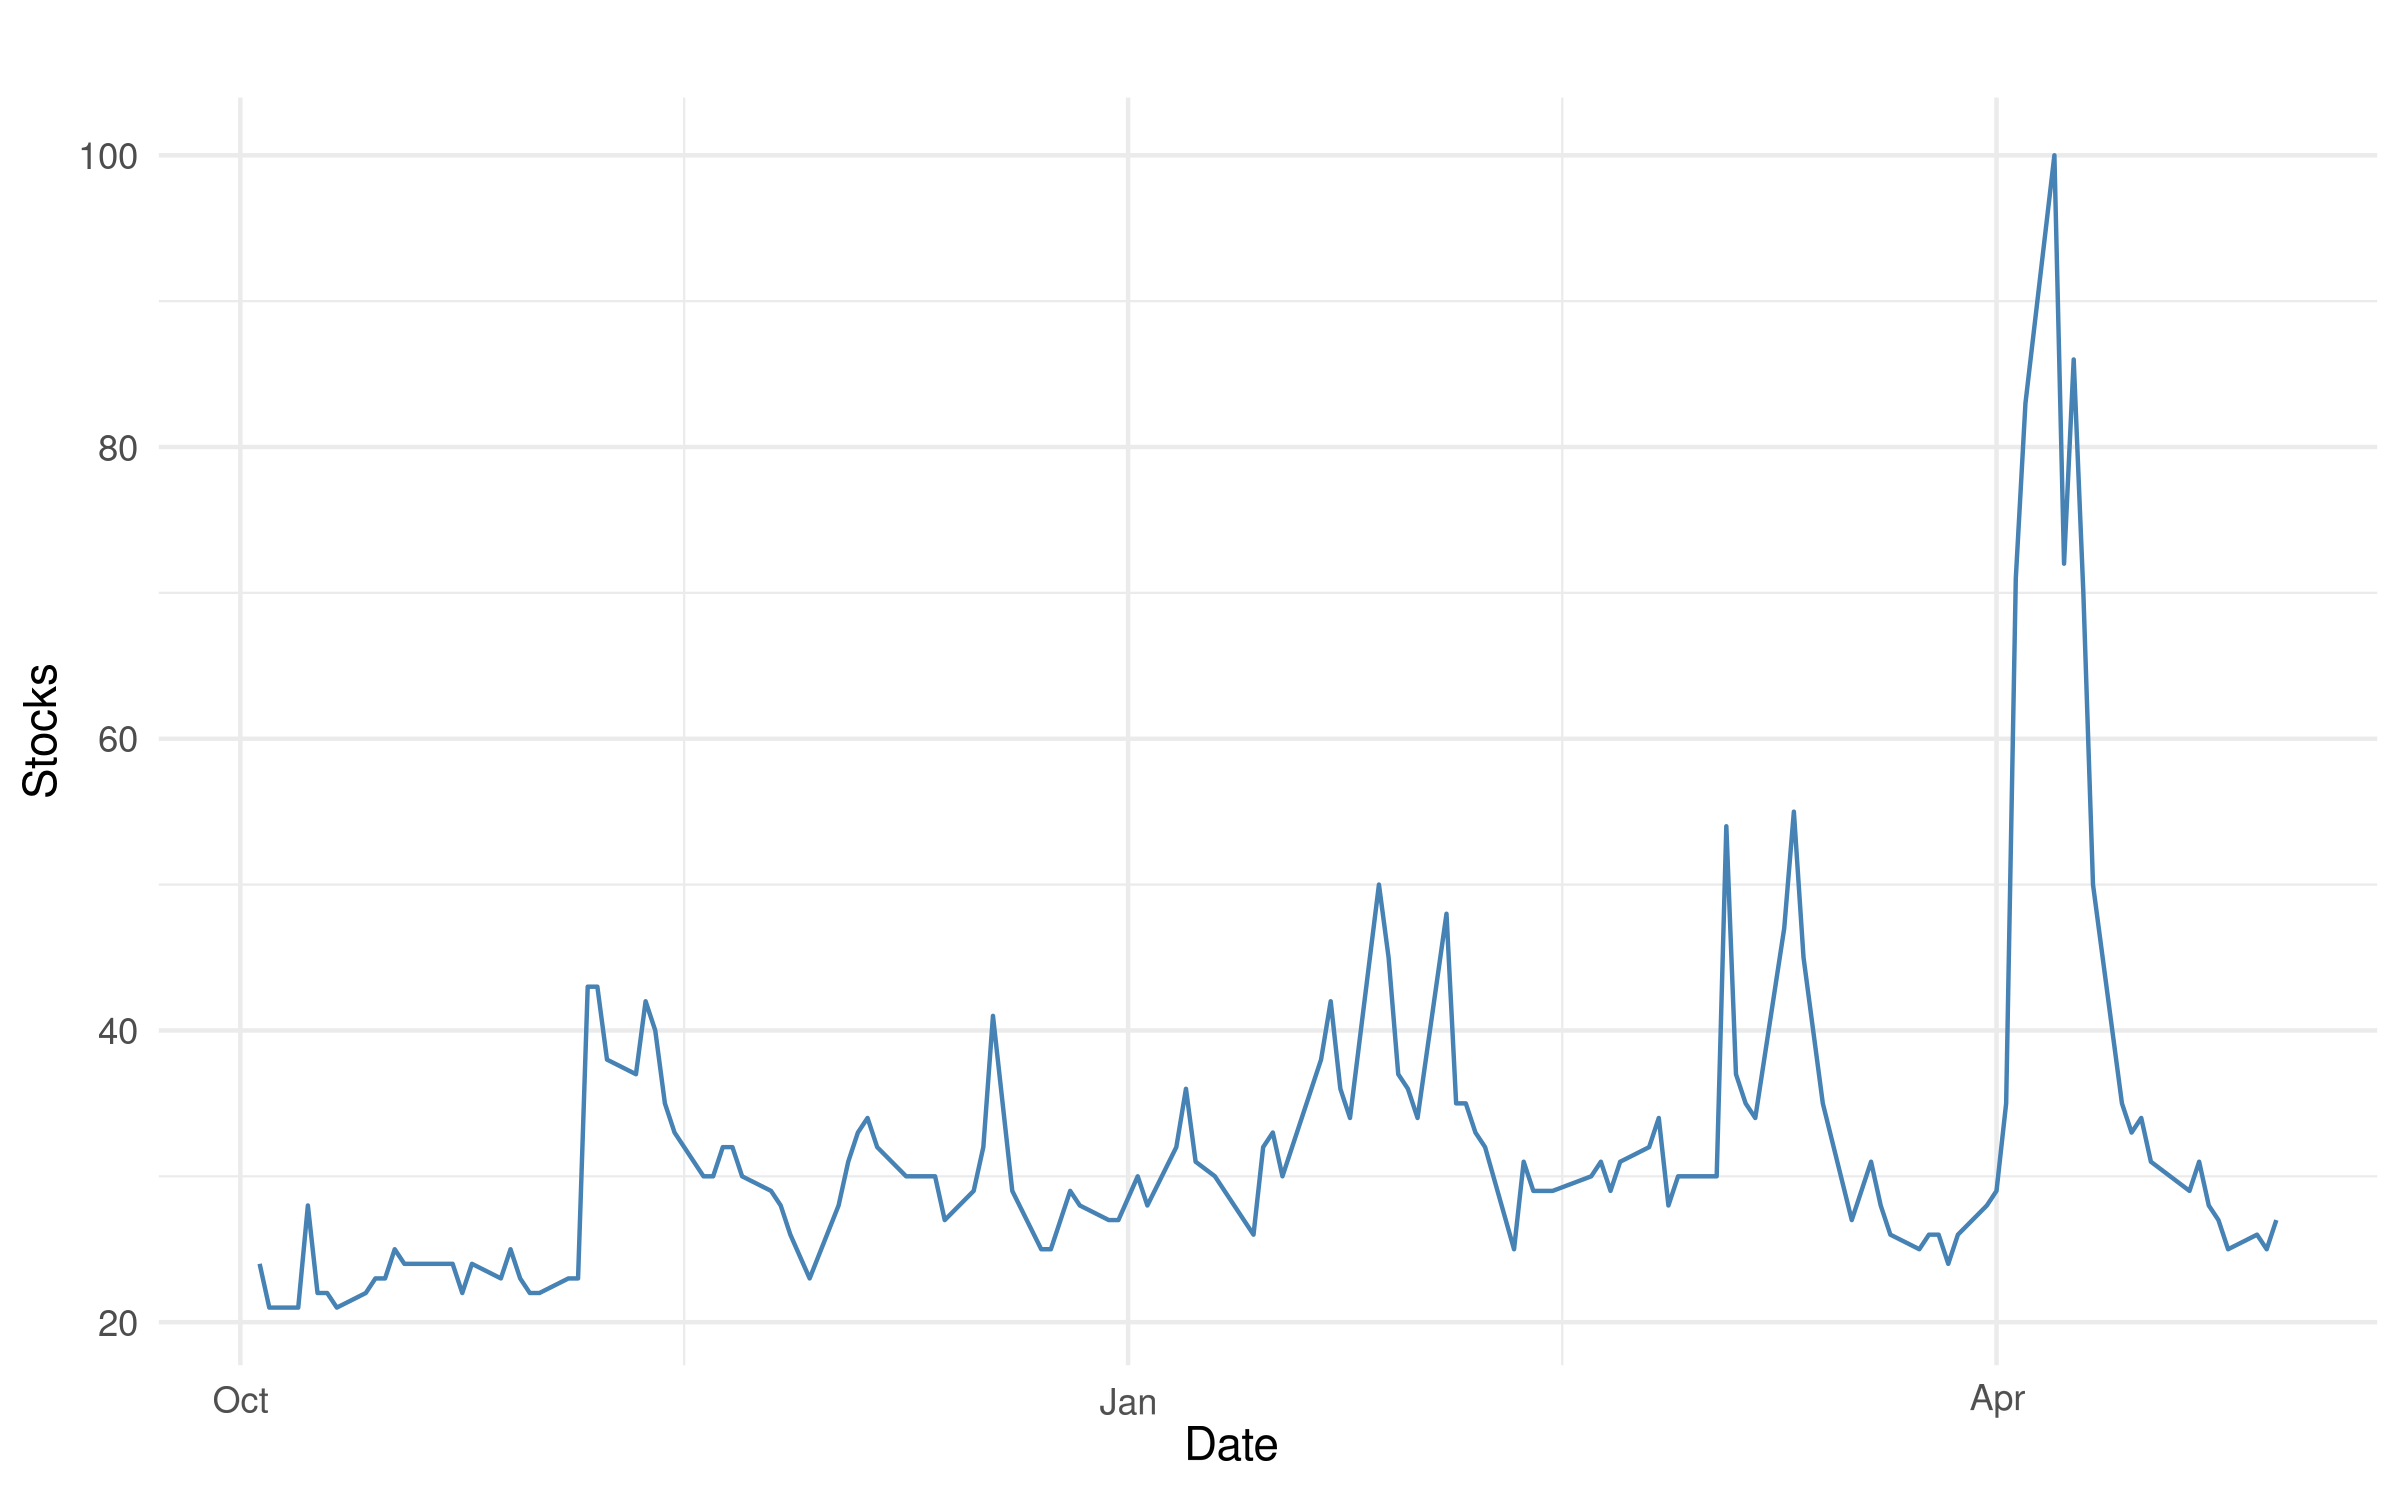
\includegraphics[width=\linewidth]{../pavic_r/Stocks_timeseries.png}
    \caption{The term "Stocks"}
    \label{fig:stocks_timeseries}
  \end{subfigure}
  \caption{Time series}
  \label{fig:histograms}
\end{figure}

Their boxplots are

\begin{figure}[H]
  \centering
  \begin{subfigure}[b]{0.48\textwidth}
    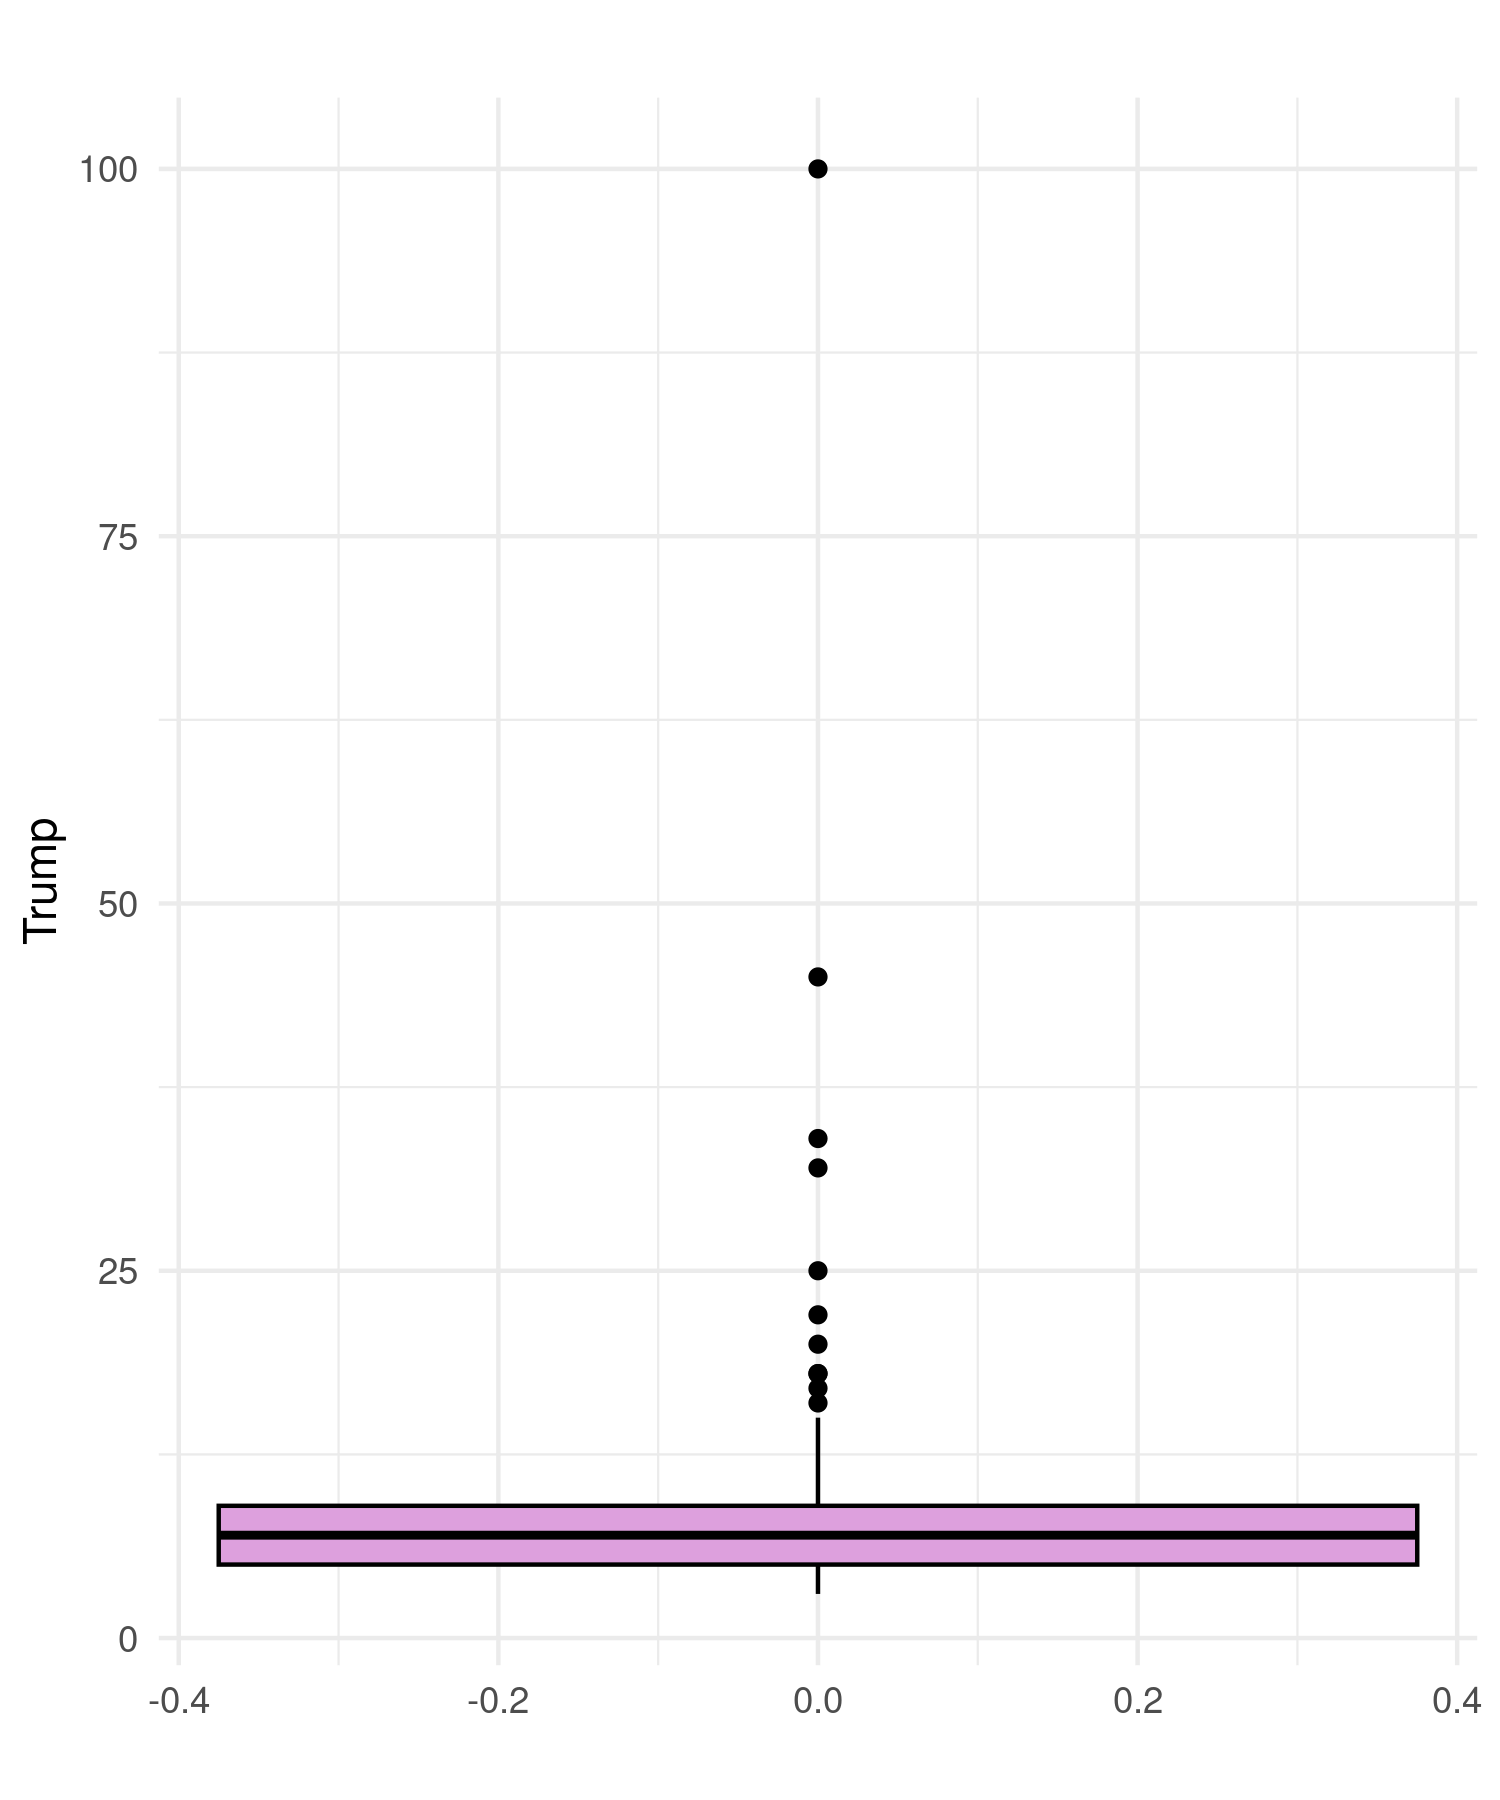
\includegraphics[width=\linewidth]{../pavic_r/Trump_boxplot.png}
    \caption{The term "Trump"}
    \label{fig:trump_boxplot}
  \end{subfigure}
  \hfill
  \begin{subfigure}[b]{0.48\textwidth}
    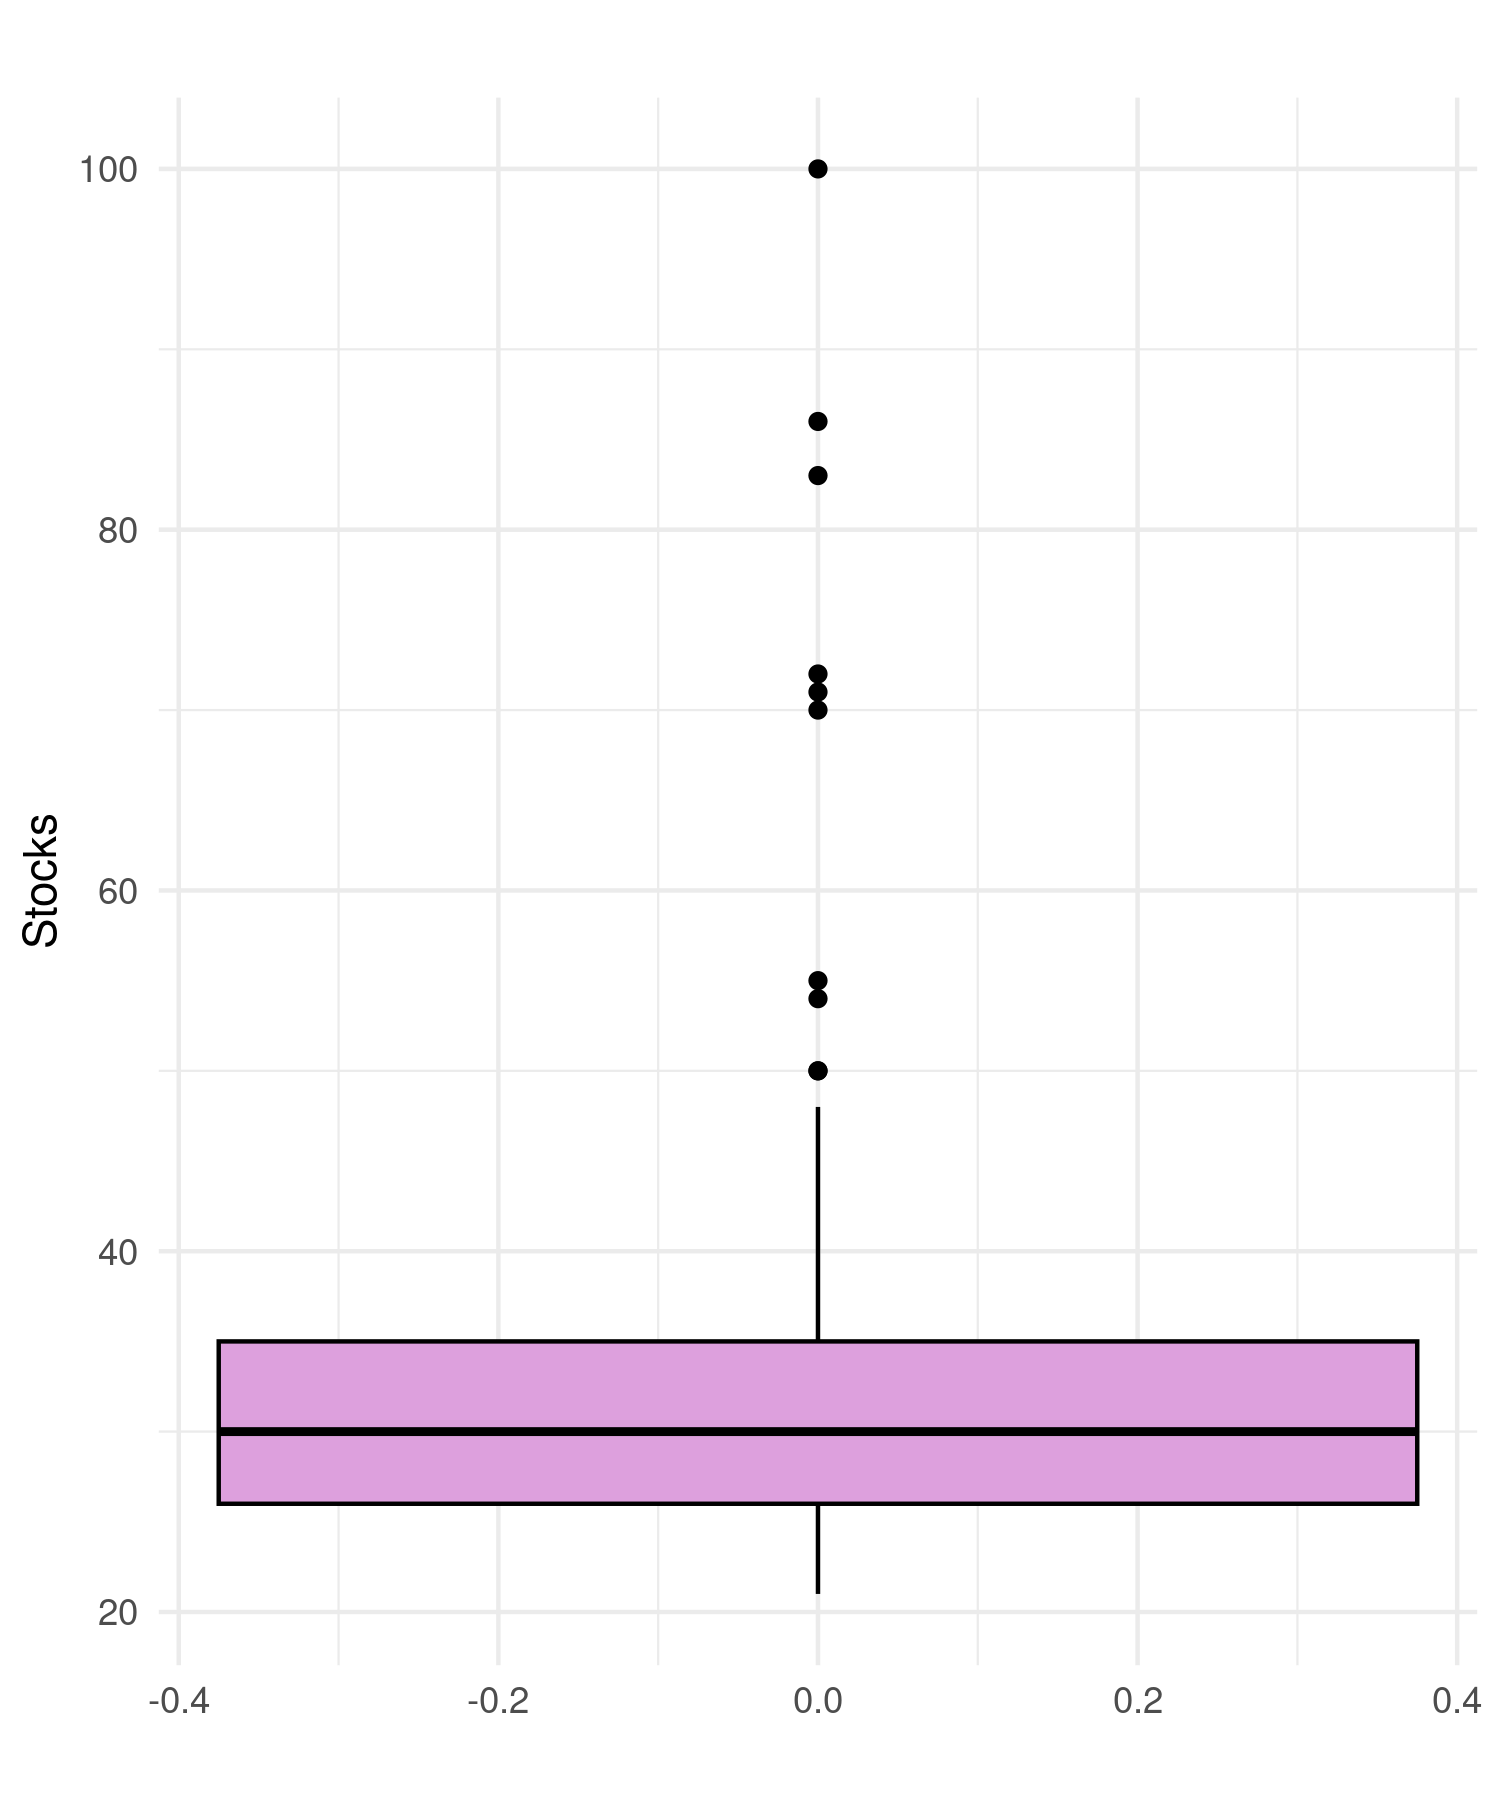
\includegraphics[width=\linewidth]{../pavic_r/Stocks_boxplot.png}
    \caption{The term "Stocks"}
    \label{fig:stocks_boxplot}
  \end{subfigure}
  \caption{Boxplots}
  \label{fig:histograms}
\end{figure}

The boxplots show that the outliers for the term "Trump" are more pronounced than those for "Stocks". The main reason is the US presidential election, held in November 2024. This corresponds exactly to the maximum frequency.

For the term "Stocks", we observe the maximum on the American "Liberation Day", the day President Trump announced his plan to introduce tariffs. Immediately afterwards, the S\&P500 experienced the third-largest three-day decline in American history. Observing this phenomenon provided our initial motivation for this seminar paper.

The five-number summary for the term "Trump" is:

\begin{align*}
(x_0(v), q_L(v), m(v), q_U(v), x_{(n)}(v)) &= (3,\; 5,\; 7,\; 9,\; 100)    
\end{align*} 
  
For the term "Stocks", it is:

\begin{align*}
(x_0(v), q_L(v), m(v), q_U(v), x_{(n)}(v)) &= (21,\; 26,\; 30,\; 35,\; 100)    
\end{align*} 

\subsection{Correlation coefficients}

Finally, we decided to examine the correlation coefficients to determine which pairs of quantities to investigate in more detail. The resulting table of coefficients is shown below.

\begin{figure}[H]
    \centering
    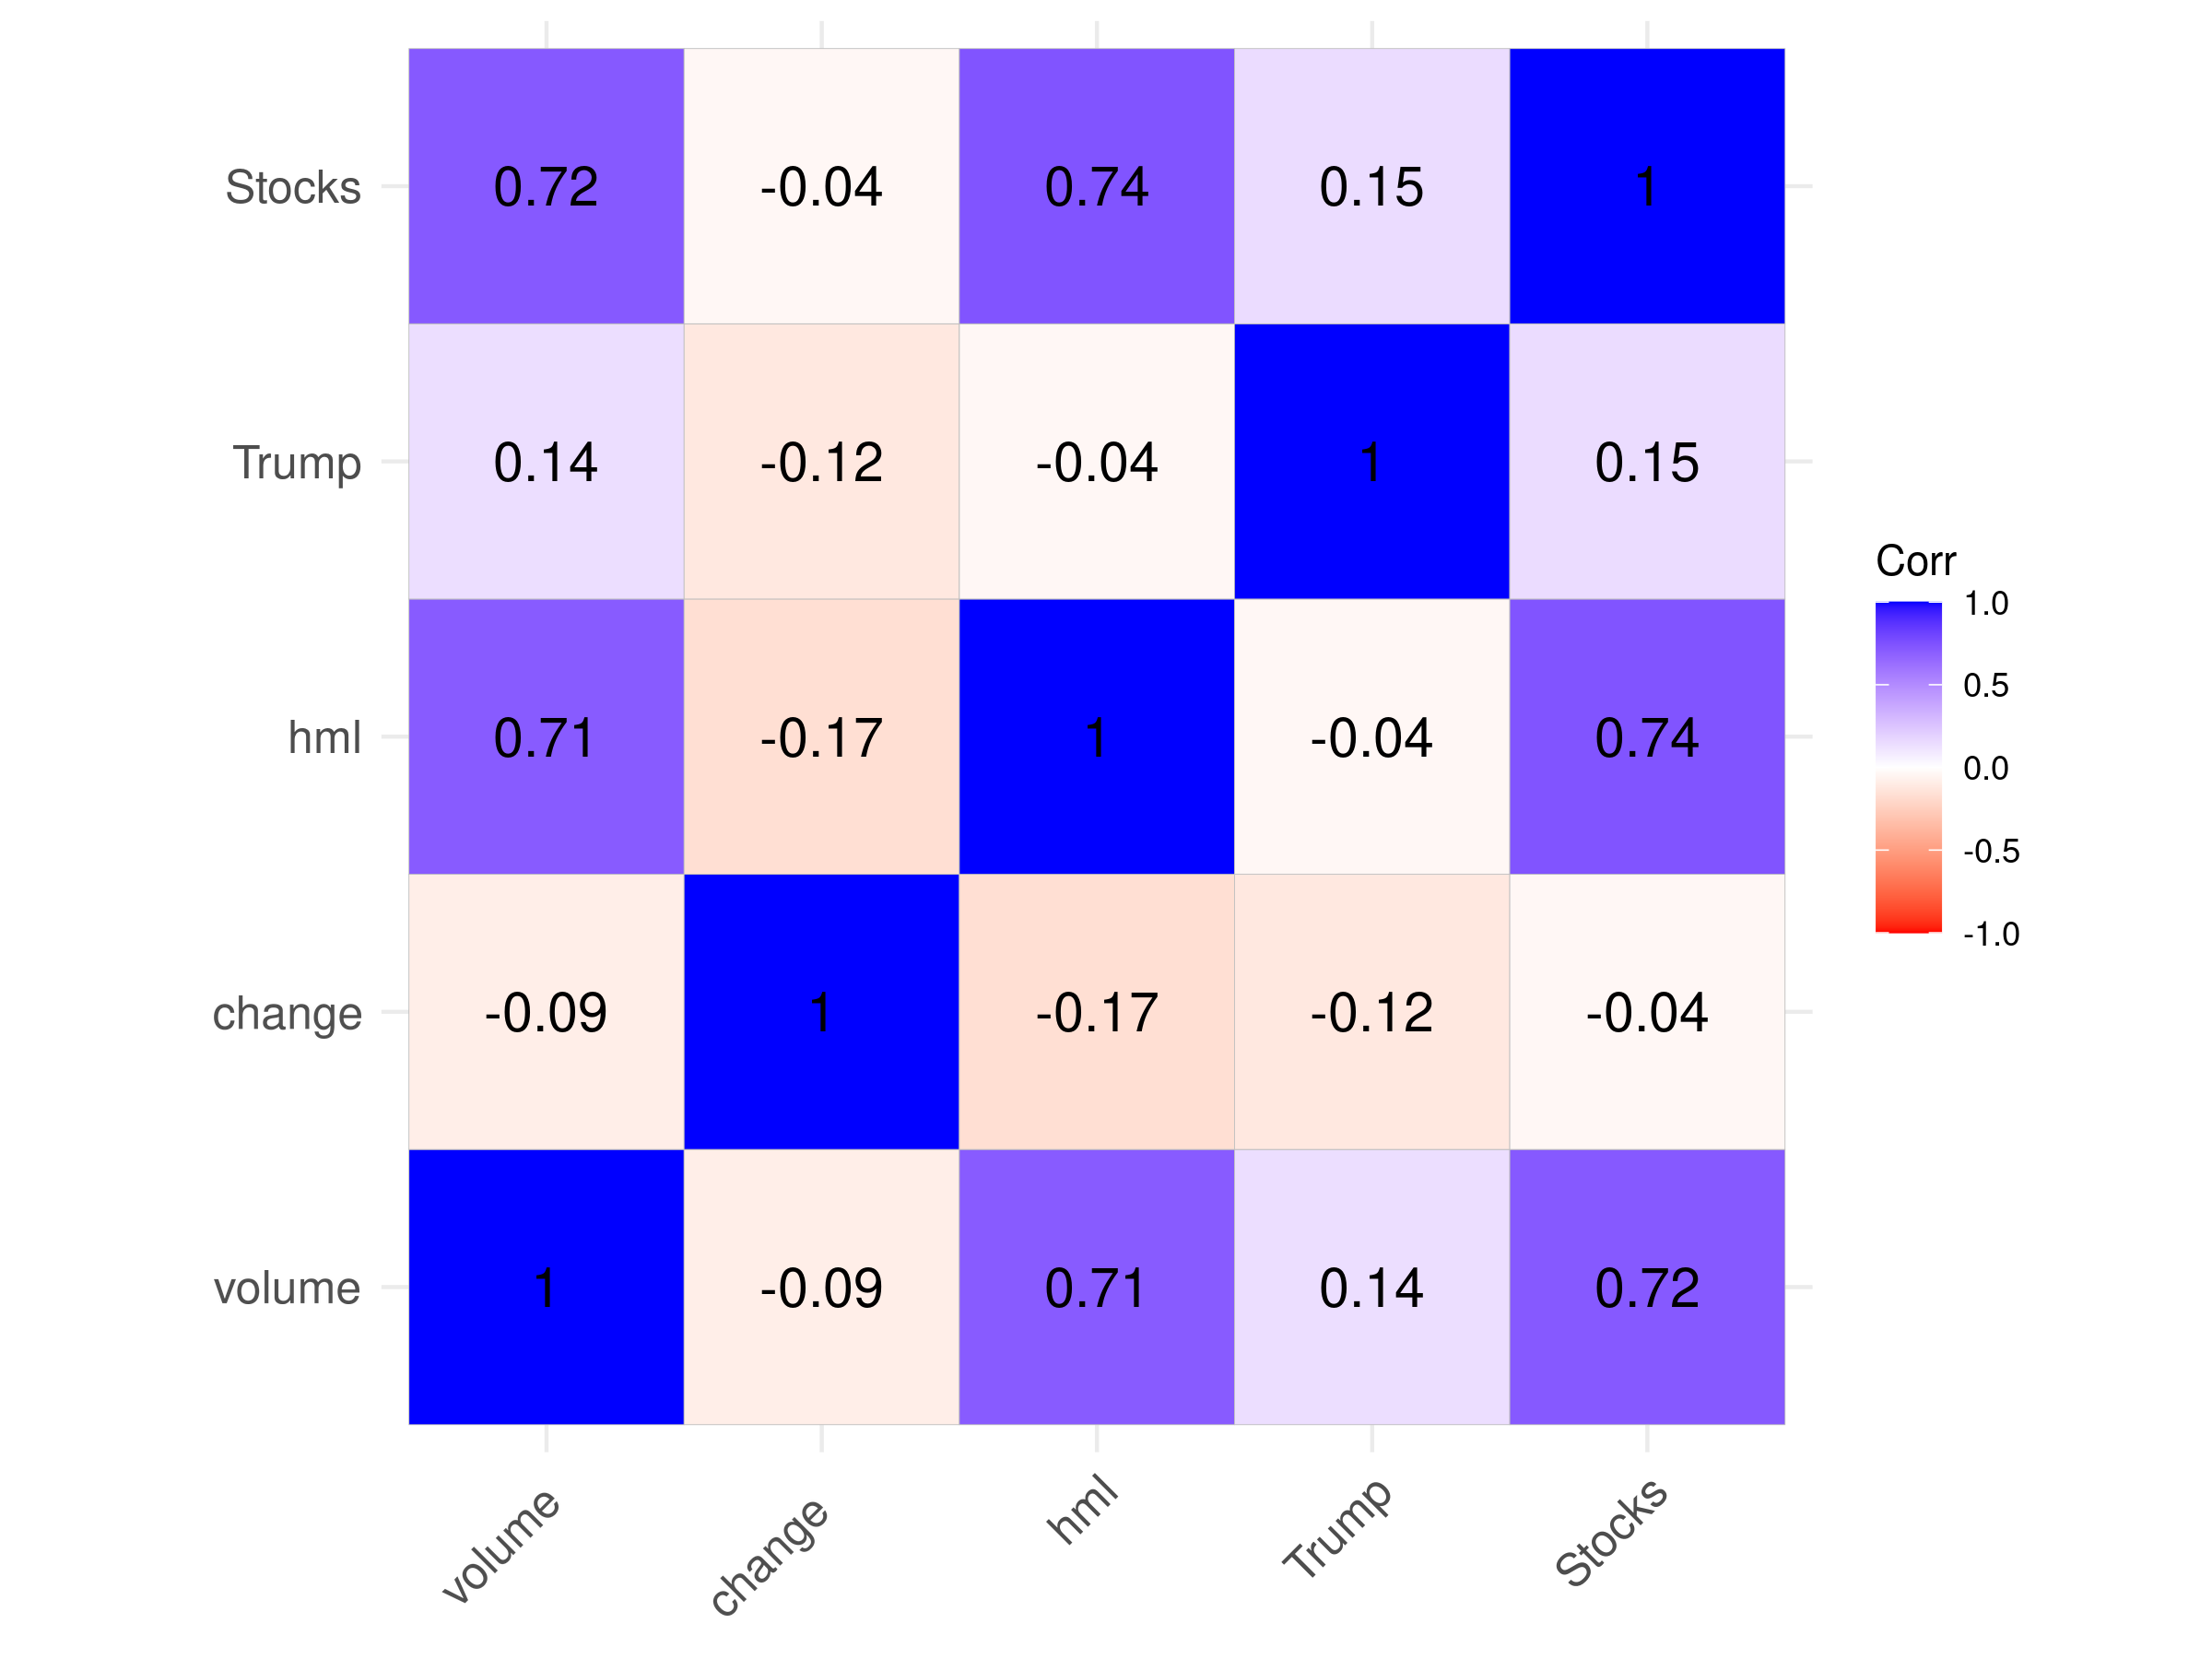
\includegraphics[width=0.6\textwidth]{../pavic_r/correlation_matrix.png}
    \caption{Correlation coefficient matrix}
    \label{fig:correlation_matrix}
\end{figure}

From this table, we concluded that change was not worth investigating much further and that the correlations with volume and hml were much stronger. Finally, we plotted four scatterplots for these pairs.

\begin{figure}[H]
  \centering
  \begin{subfigure}[b]{0.48\textwidth}
    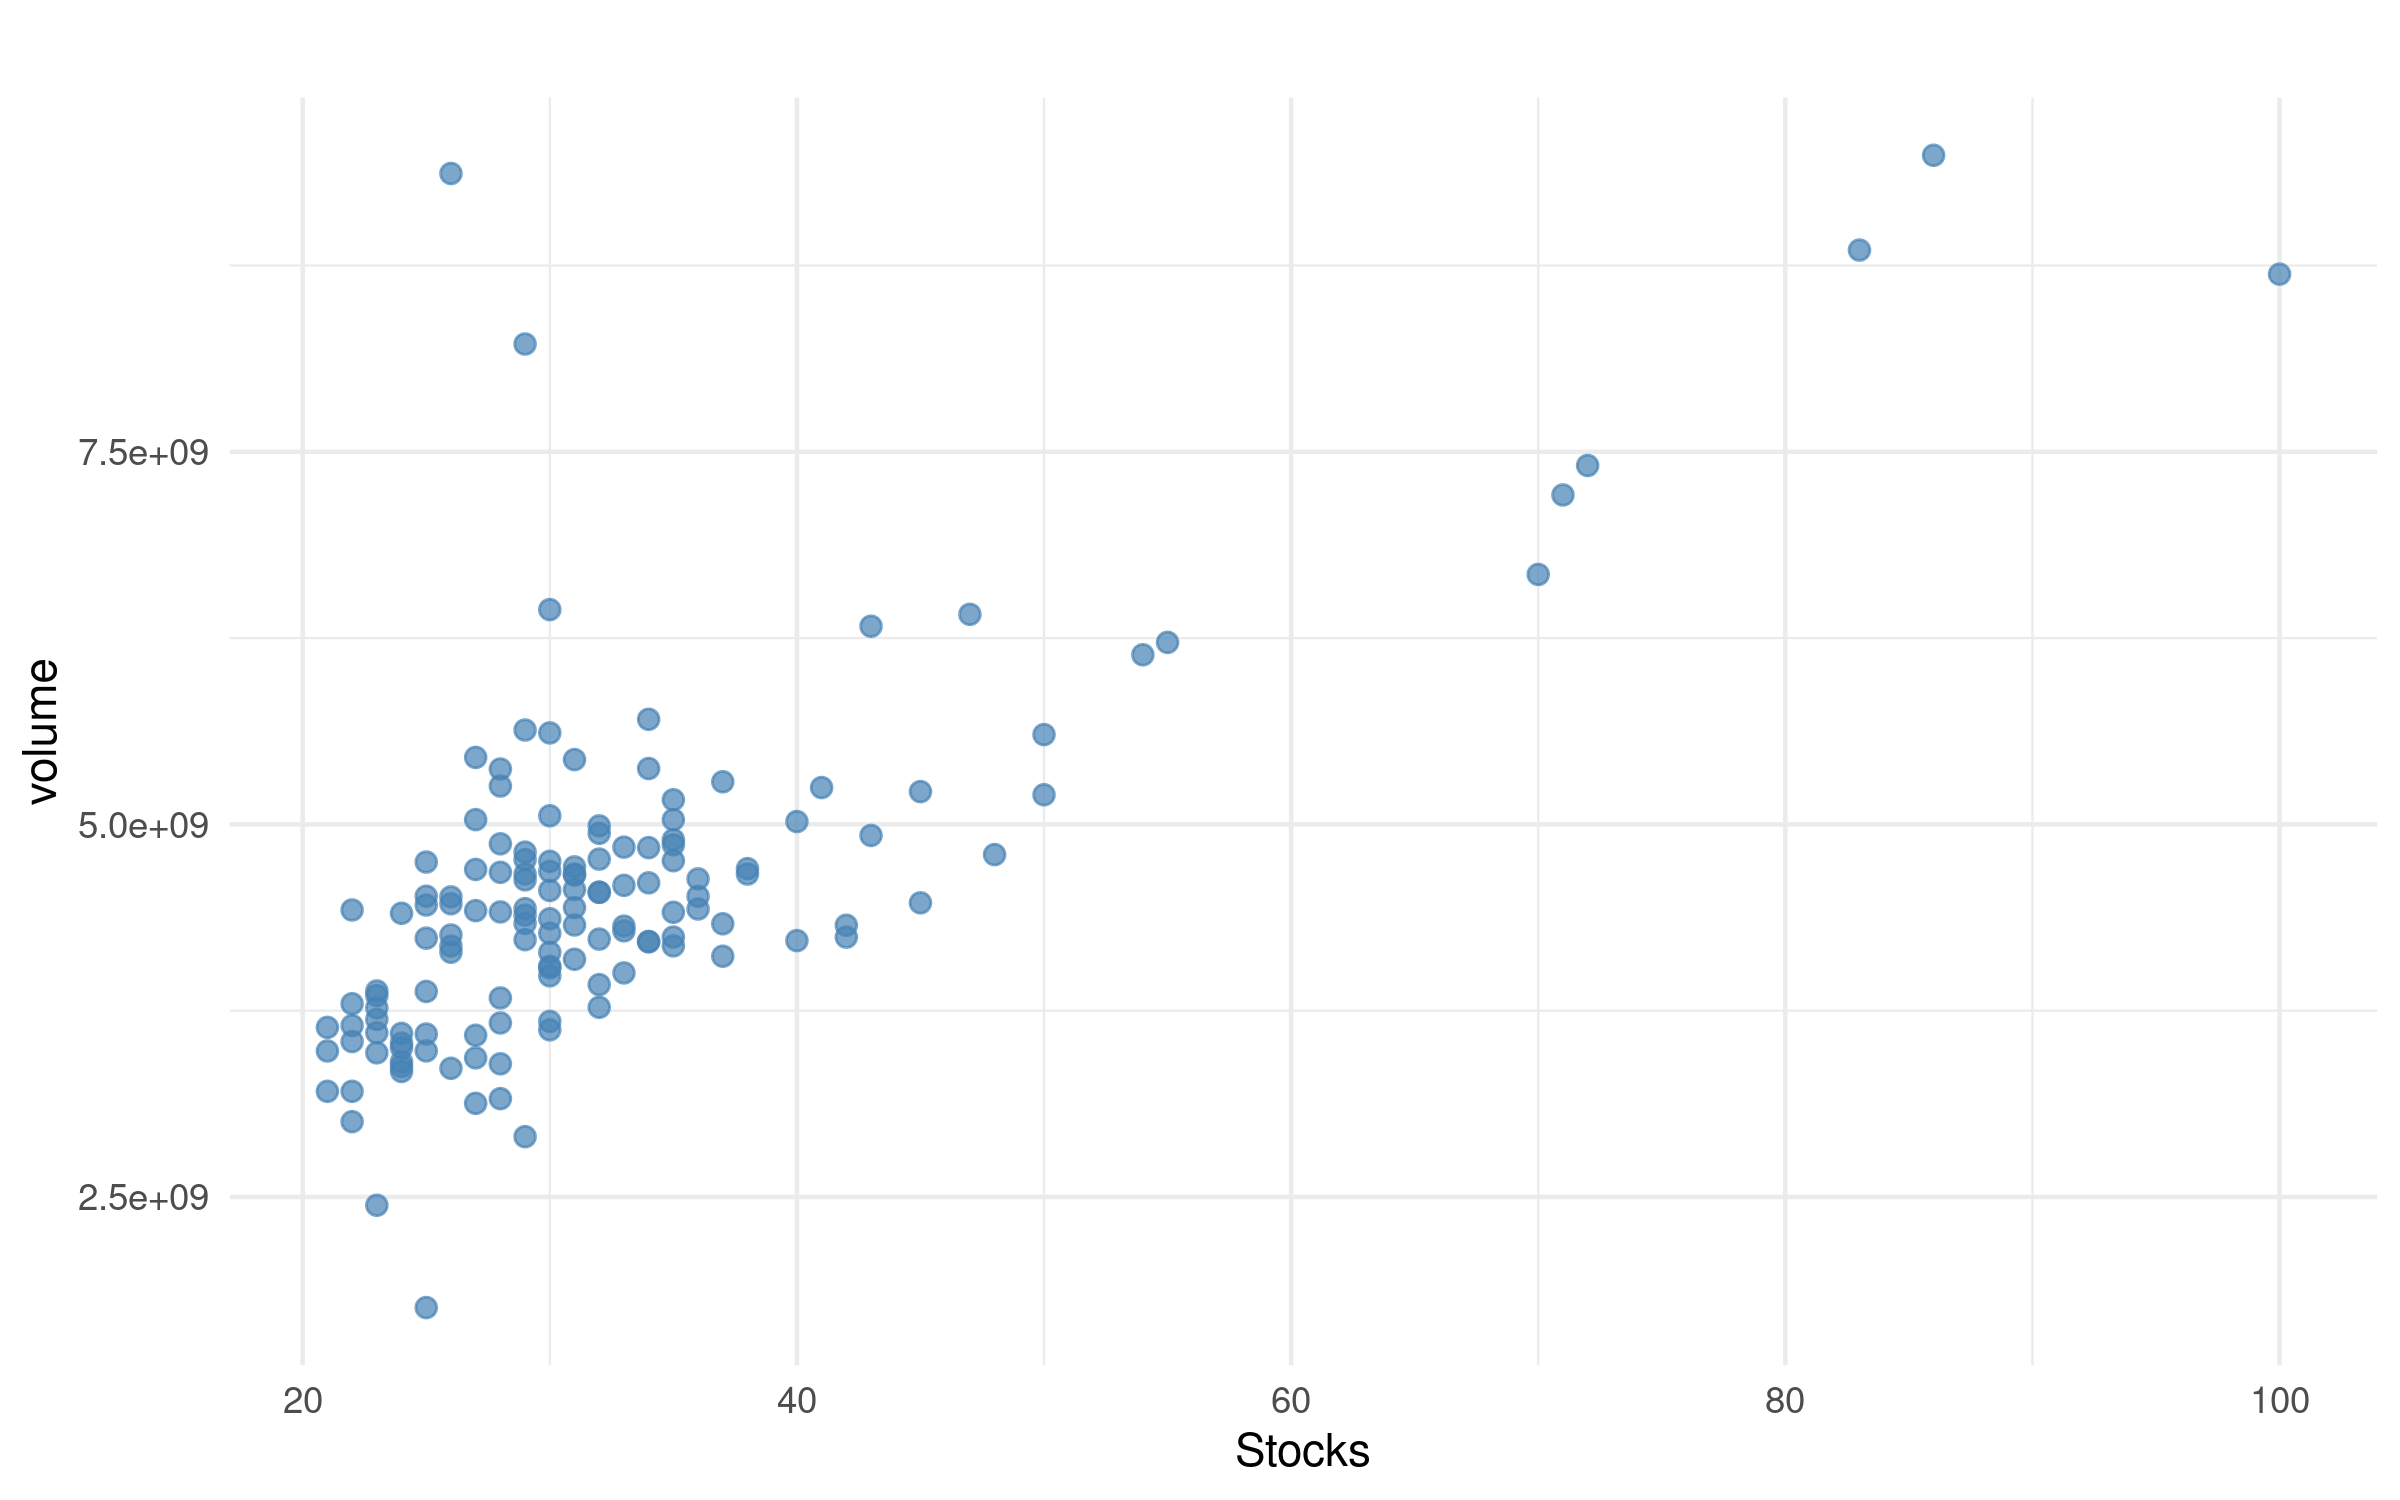
\includegraphics[width=\linewidth]{../pavic_r/scatterplot_Stocks_vs_volumen.png}
    \caption{Stocks --- volume}
    \label{fig:scatterplot_Stocks_volumen}
  \end{subfigure}
  \hfill
  \begin{subfigure}[b]{0.48\textwidth}
    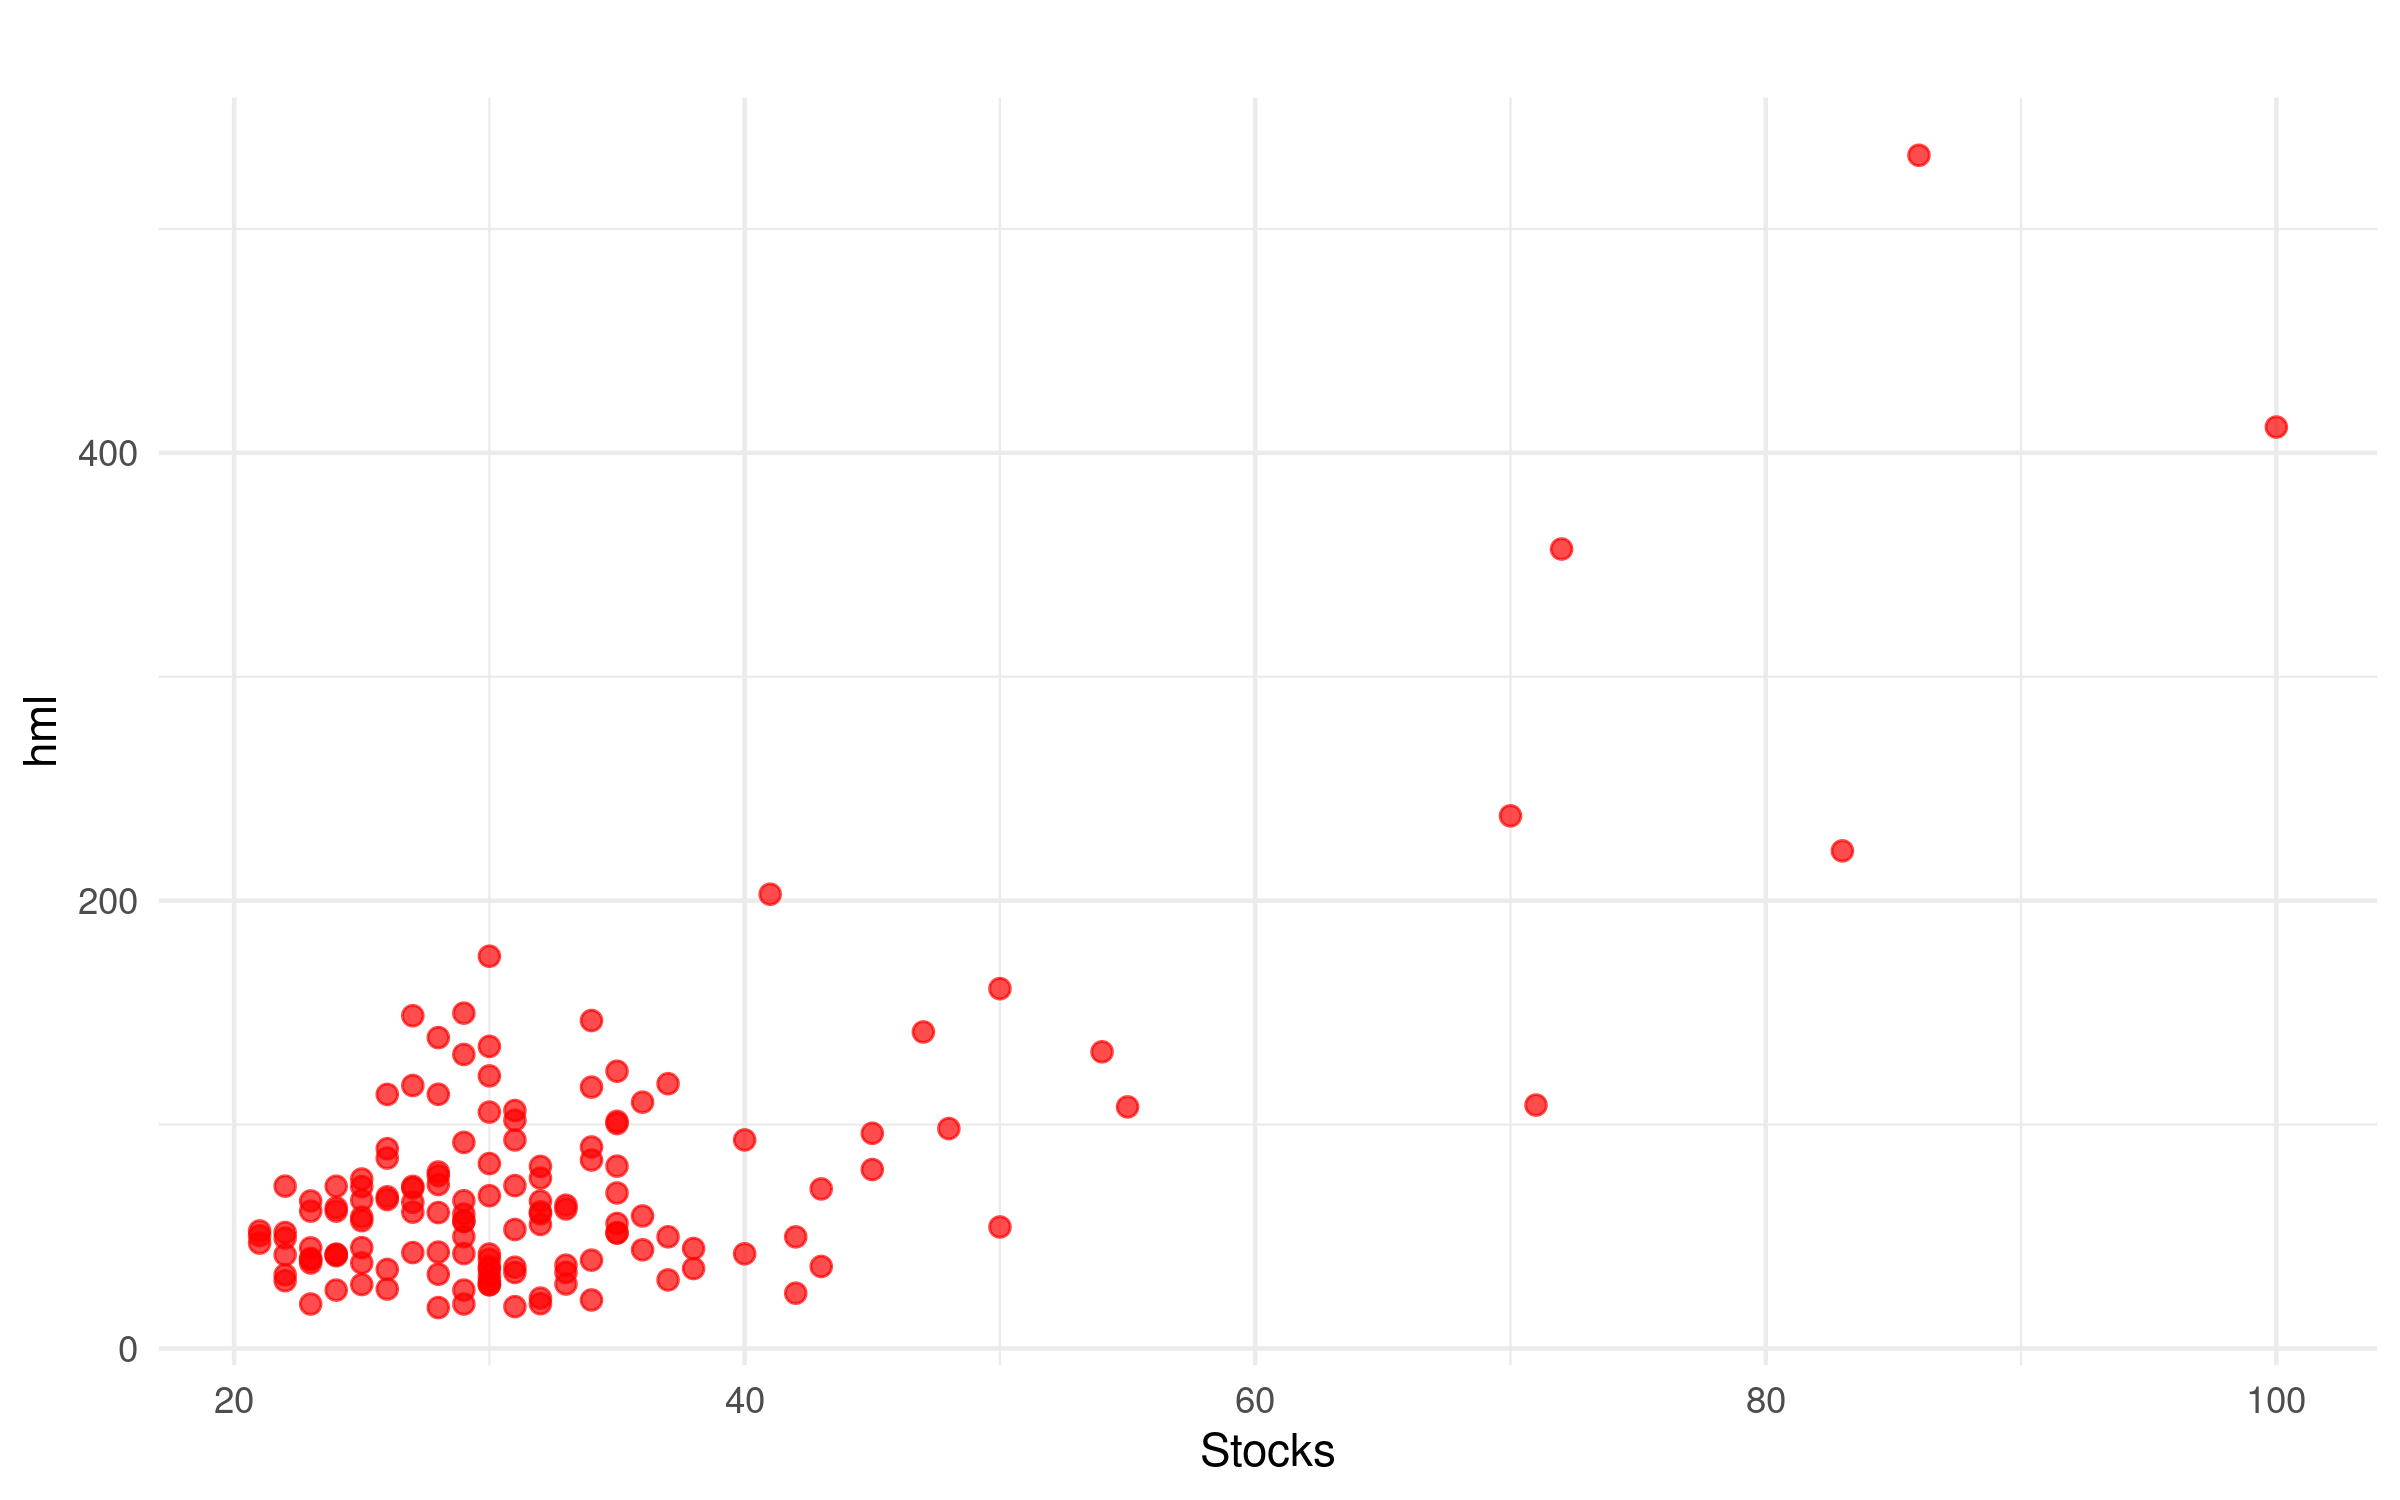
\includegraphics[width=\linewidth]{../pavic_r/scatterplot_Stocks_vs_hml.png}
    \caption{Stocks --- hml}
    \label{fig:scatterplot_Stocks_hml}
  \end{subfigure}
  
  \begin{subfigure}[b]{0.48\textwidth}
    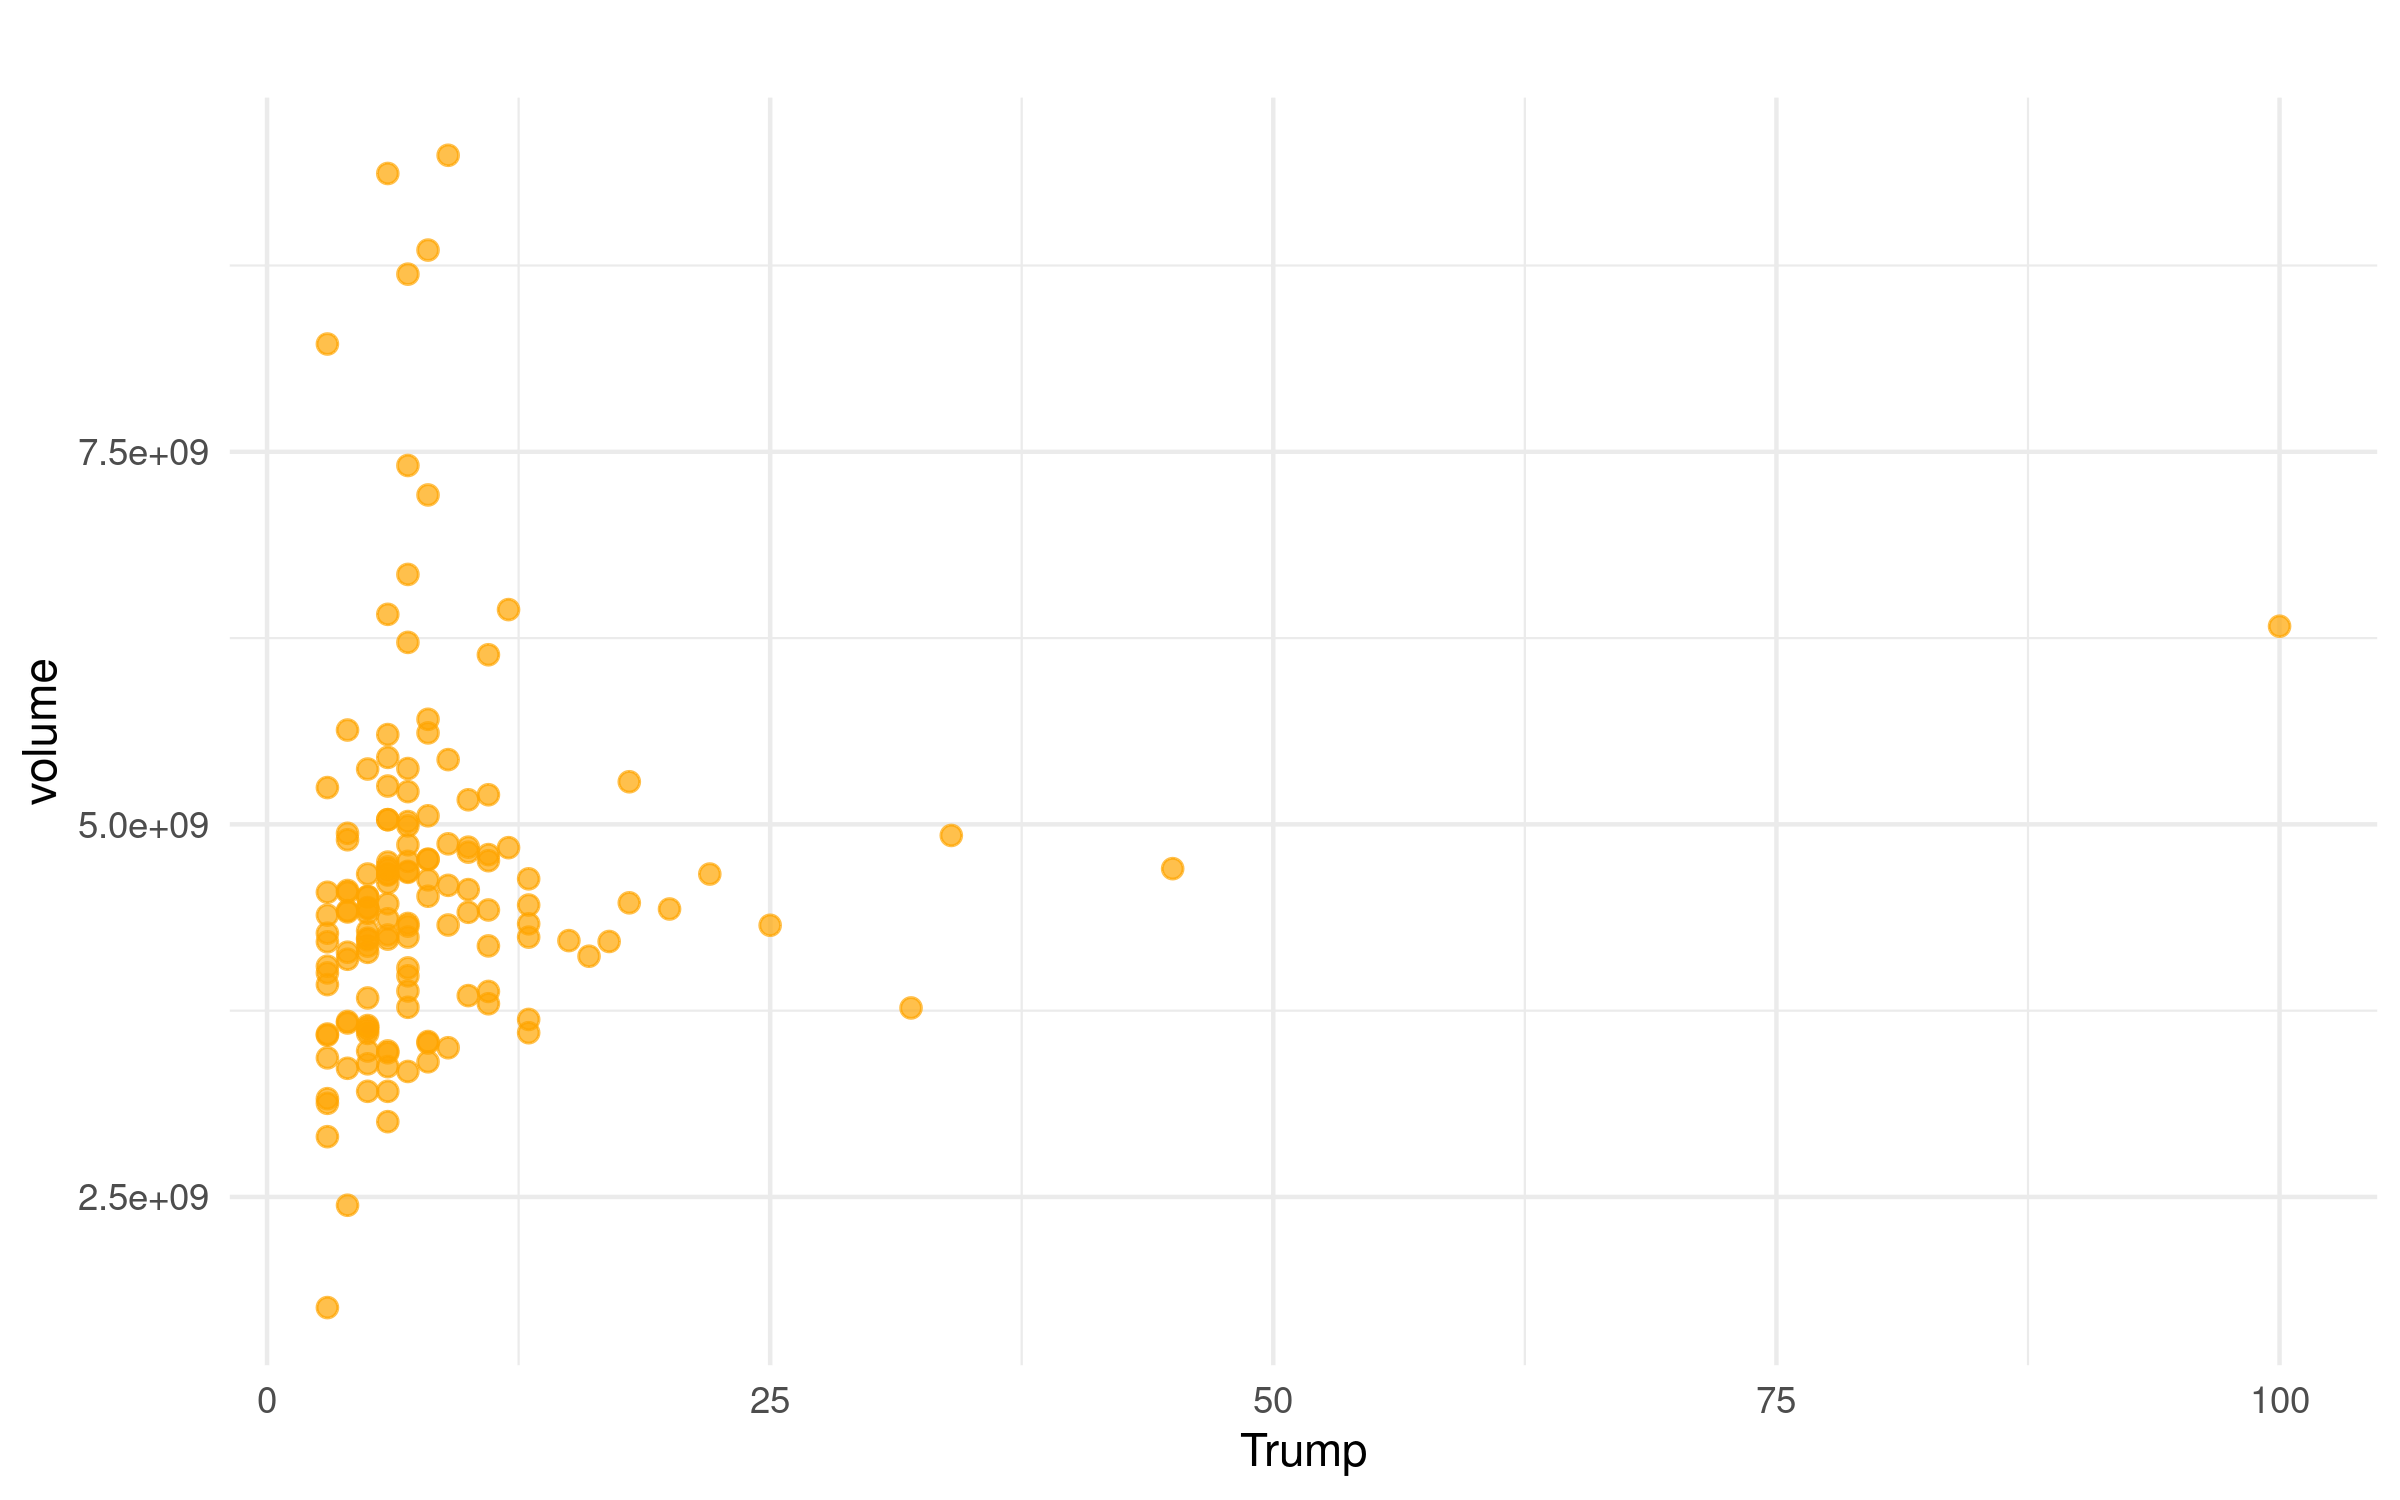
\includegraphics[width=\linewidth]{../pavic_r/scatterplot_Trump_vs_volumen.png}
    \caption{Trump --- volume}
    \label{fig:scatterplot_Trump_volumen}
  \end{subfigure}
  \hfill
  \begin{subfigure}[b]{0.48\textwidth}
    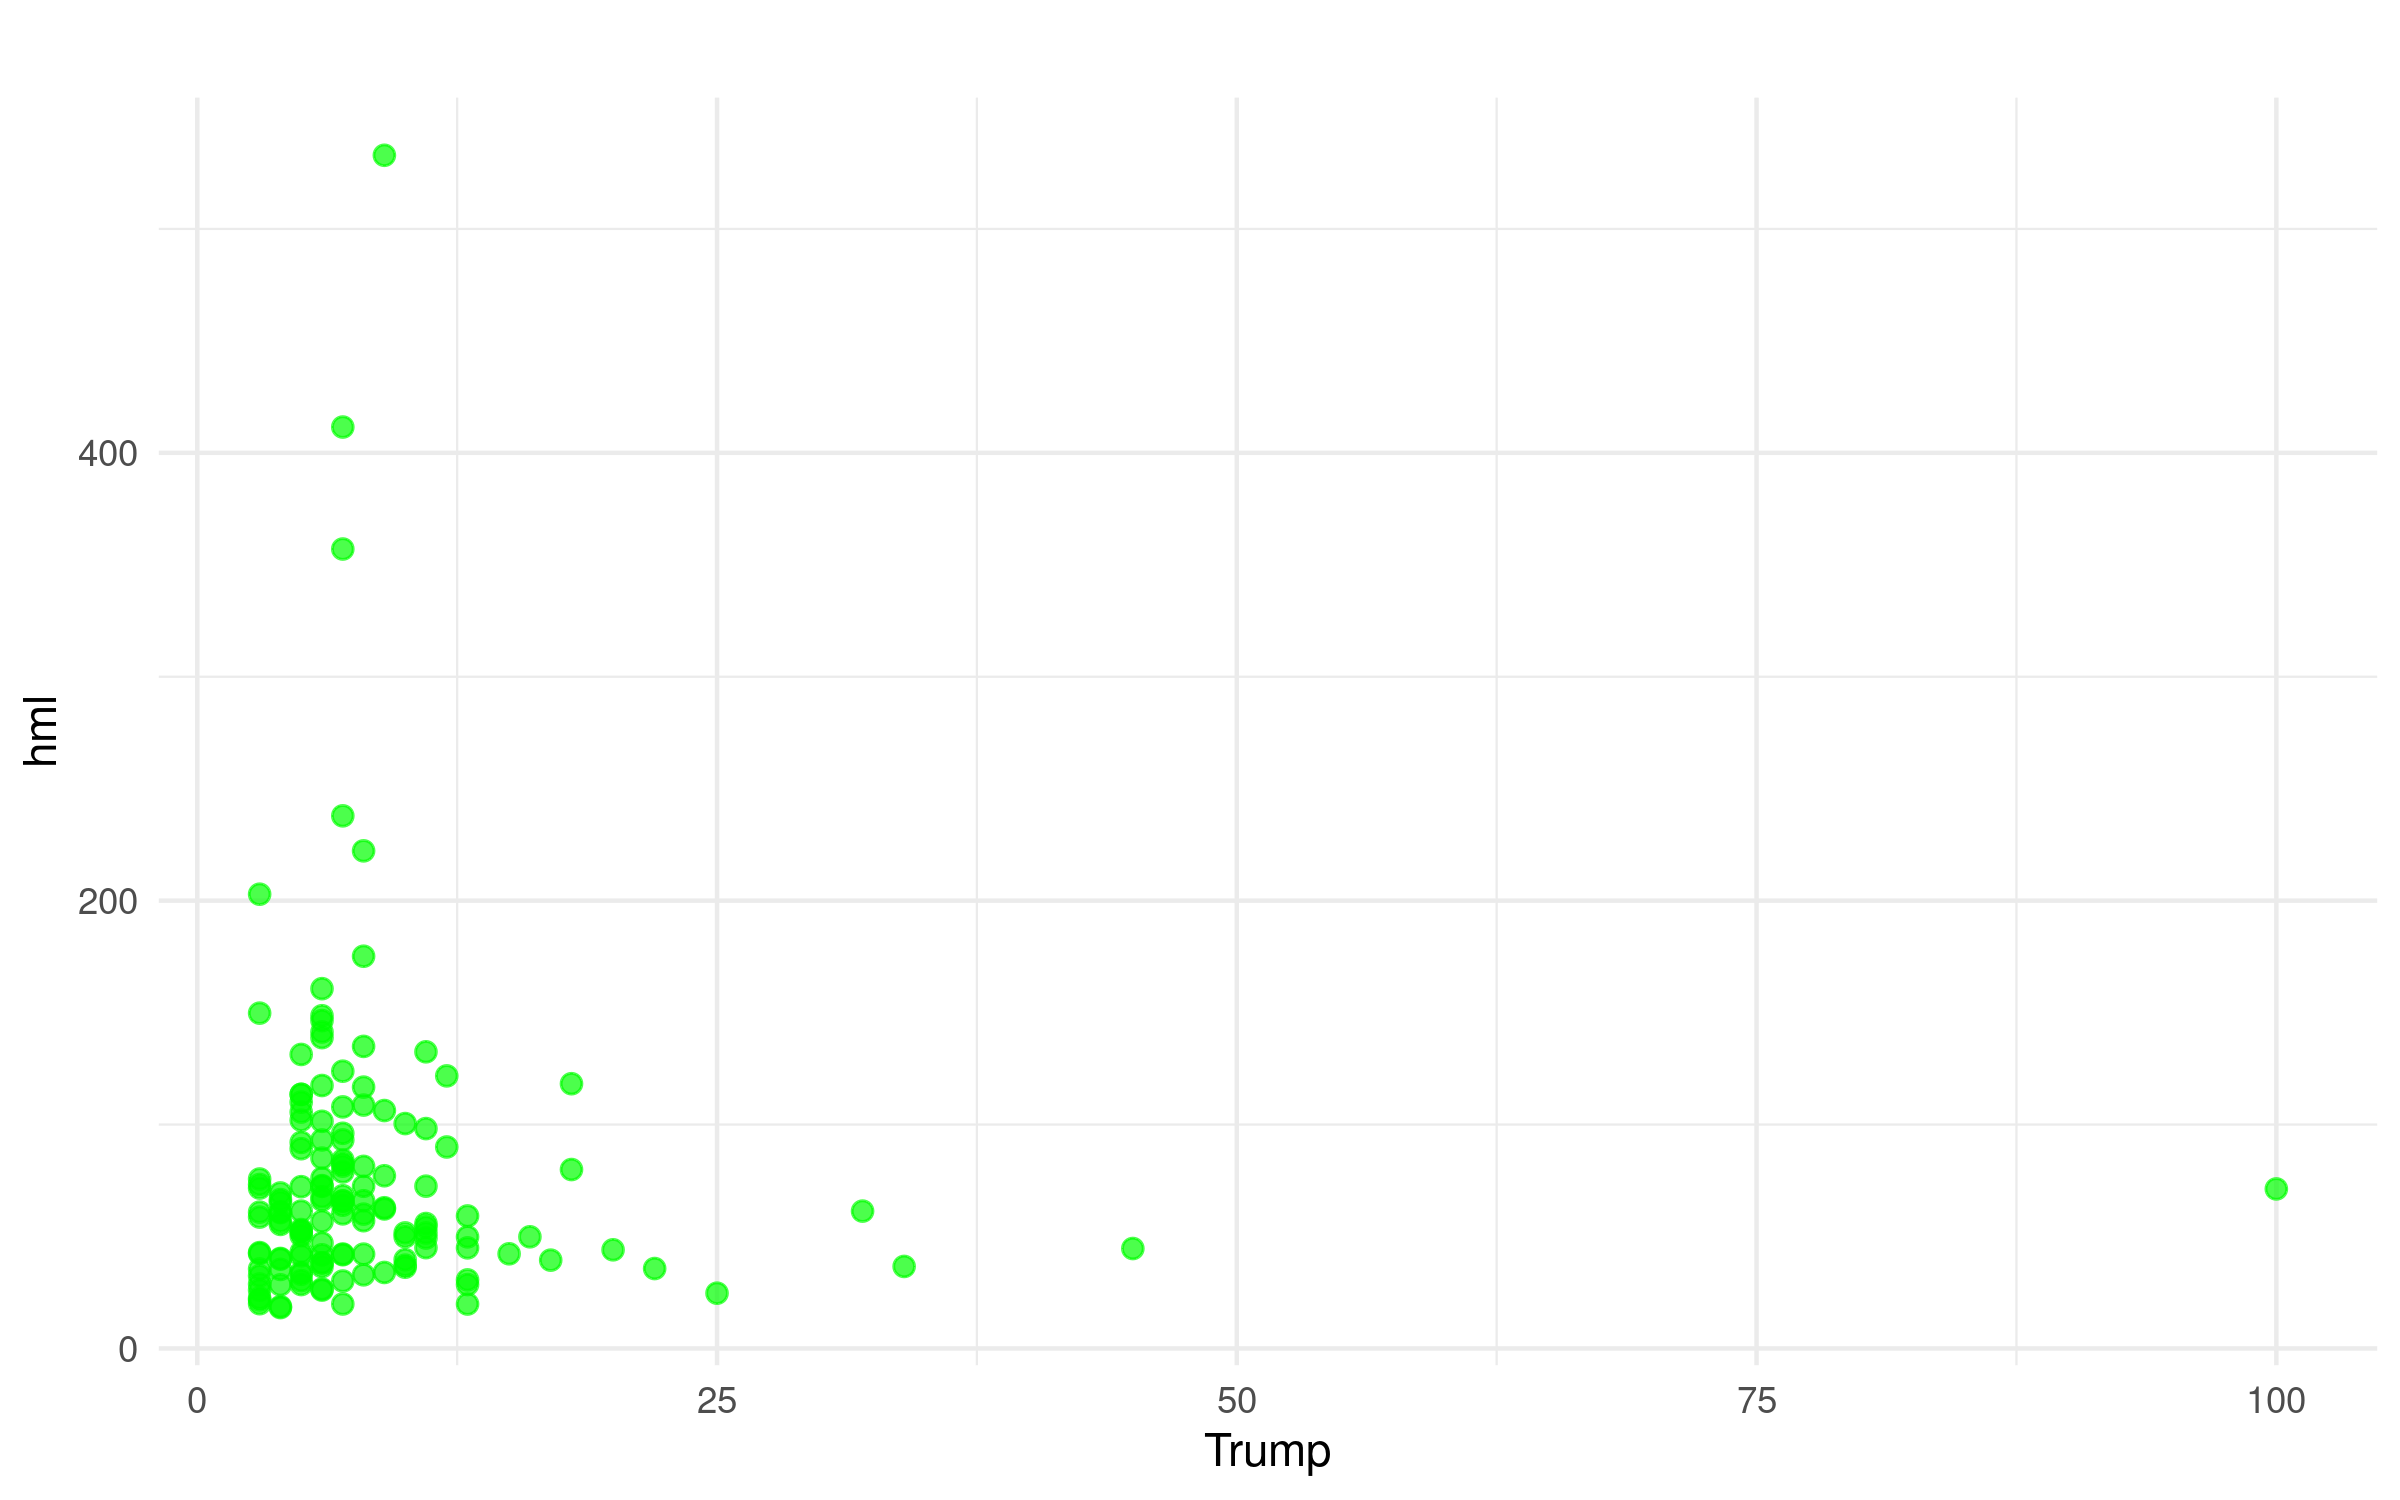
\includegraphics[width=\linewidth]{../pavic_r/scatterplot_Trump_vs_hml.png}
    \caption{Trump --- hml}
    \label{fig:scatterplot_Trump_hml}
  \end{subfigure}
  
  \caption{Scatterplots}
  \label{fig:histograms}
\end{figure}



\end{document}